
\documentclass[conference]{IEEEtran}

%\usepackage{ifpdf}
\usepackage{float}  % For handling float environments like [H]
\usepackage{url}    % For handling URLs
\usepackage{multirow}
\usepackage{subcaption} % Required for subfigures
\usepackage{booktabs}
\usepackage{cite}
\pagestyle{plain}
\usepackage{amsmath}
\usepackage{float}
\usepackage{tikz}
\usetikzlibrary{shapes.geometric, arrows, positioning}%\usepackage{url}


\ifCLASSINFOpdf
  \usepackage[pdftex]{graphicx}
  % declare the path(s) where your graphic files are
  % \DeclareGraphicsExtensions{.pdf,.jpeg,.png}
%\else
  % or other class option (dvipsone, dvipdf, if not using dvips). graphicx
  % and their extensions so you won't have to specify these with
  % every instance of \includegraphics
  % \DeclareGraphicsExtensions{.eps}
\fi
% graphicx was written by David Carlisle and Sebastian Rahtz.


% correct bad hyphenation here
\hyphenation{op-tical net-works semi-conduc-tor}


\begin{document}


\title{Applying ML to assess fatigue and prevent injury\\in high performance swimming athletes}

% use a multiple column layout for up to three different
% affiliations
\author{\IEEEauthorblockN{Hugo Veríssimo}
\IEEEauthorblockA{Foundations of Machine Learning 24/25\\
University of Aveiro\\
Aveiro, Portugal\\
hugoverissimo@ua.pt}
\and
\IEEEauthorblockN{João Cardoso}
\IEEEauthorblockA{Foundations of Machine Learning 24/25\\
University of Aveiro\\
Aveiro, Portugal\\
joaopcardoso@ua.pt}}


% make the title area
\maketitle
\thispagestyle{plain}

% As a general rule, do not put math, special symbols or citations
% in the abstract
\begin{abstract}
temos que arranjar refs para ir metendo por ai
\end{abstract}
Não esquecer de definir abreviaturas na primeira ocorrência e usá-las daí em diante.


\begin{quote}
\small
\noindent
\textbf{Keywords:} Your, Keywords, Go, Here
\end{quote}

\IEEEpeerreviewmaketitle


\section{Introduction}
The evolution in performance of high level athletes is highly dependent on their skill, motivation, and discipline. With the support of a knowledgeable coach, the evolution can be substantially improved, through careful tailoring of the training regimen. One of the most relevant metrics since the dawn of structure training in sports is the feedback from the athlete, commonly described as the rate of perceived exertion (RPE). This single metric comprises the athletes analysis and intuition of the effort that was carried and how ready they feel for another bout of training. In recent years, more and more sports coaches have relied heavily on collected data to better assess, plan and adjust the training plans of their athletes in a systematic way. This allows for a fine balance between intense workouts, that generate stronger stimuli for muscle development and sport specific skills, taking the balance between effort and fatigue as the crucial ratio to respect. Too high effort, may lead to injury, too low and some gains may be left on the table. 

In the scope of the first project for Foundations of Machine Learning, we decided to partner with the local sports club CAPGE (Clube Associação de Pais da Gafanha da Encarnação) to treat the data (kindly shared by Sr Coach Daniel Tavares) for estimating the fatigue of several athletes. The data was curated and prepared to implement and fit several machine learning algorithms to estimate fatigue after workout.

With this approach, we aim to generalize the models for different athletes/sports, and make it available to the local club for implementation and further testing. 



\section{State of the Art}

Over the past decade there have been significant improvements in the field of ML applied algorithms for sports' related applications. Here we present the most relevant work in fatigue and injury prediction, which is not specifically on the sport we're assessing in our dataset, which lead to additional interpretations from the works analyzed to our own case of study. In general, the problem of class imbalance is seen throughout the literature, and different solutions are proposed, such as data gathering and preprocessing, over sampling and under sampling, with SMOTE (synthetic minority over-sampling technique) being the most commonly used approach for over sampling. As early as 2010, Gabbet and colleagues modeled the risk of injury with a monodimensional approach using logistic regression, based on athletes rate of perceived exertion, showing that even with a monovariate approach to injury prediction useful results could be attained. In recent years, several authors have focused in alternative techniques such as Logistic Regression, Random Forest, Support Vector Machine, or Convolutional Neural Network on Multivariate Timeseries (the references for these papers can be found in the paper "A Narrative Review").

Besides model selection, feature engineering and selection is among the most debated topics. Several authors opt to include GPS data, metabolic consumption, mechanical load, RPE, detailed quantification of workloads, ratio between acute:chronice loads. Despite the multivariate imputation, data analysis often shows strong correlations between them, leading to over fitting problems (usually model independent).

In the work by Carey et al. (2018) different algorithms have been implemented to predict the risk of injury in an Australian football club. The data collection lasted for three seasons, consisting of absolute and relative training load metrics, derived from GPS, accelerometer, and RPE data. The prediction models used were regularized logistic regression, generalized estimating equations, random forests, and support vector machines, with periods of 3, 6, and 21 days (these periods have been studied and verified as adequate for the case of Australian football). The periods served to calculate moving averages and exponentially weighted moving averages (EWMA). The latter allowed to account for the decay in significance of the training load the further it happened from a given day, in accordance with the work from Williams et al. (2016). From the results it was possible to verify that over fitting was very likely due to the multicollinearity between variables, which was confirmed by principal component analysis (PCA). The use of PCA with regularized logistic regression slightly improved the results.

More recent studies have employed ensemble algorithms, in order to take most of the different learning models selected, taking into account the need to balance the classes as is common practice for this type of problems. 

In summary, the integration of machine learning techniques in sports fatigue and injury prediction has evolved from simple monovariate models to complex multivariate and ensemble approaches. Addressing challenges such as class imbalance, feature selection, and multicollinearity remains crucial for developing robust predictive models applicable across different sports contexts.

\section{Methodology}
The methodology defined for this project consisted of three major steps: assessment and curation of the dataset, feature engineering and selection of features, followed by data normalization; training of the selected machine learning models; finalizing with model evaluation and subsequent training until optimum results were achieved. Figure~\ref{fig:methodology} illustrates the methodology used in this project.

% TikZ styles
\tikzstyle{startstop} = [rectangle, rounded corners, minimum width=2.5cm, minimum height=1cm, text centered, draw=black, fill=red!30]
\tikzstyle{process} = [rectangle, minimum width=2.5cm, minimum height=1cm, text centered, draw=black, fill=blue!30]
\tikzstyle{arrow} = [thick,->,>=stealth]

\begin{figure}[h]
\centering
\resizebox{\columnwidth}{!}{ % Resize to fit column width
\begin{tikzpicture}[node distance=1.5cm, font=\scriptsize] % Adjust font size to match document

% Nodes
\node (start) [startstop] {Raw data};
\node (curation) [process, below of=start] {Data Assessment \& Curation};
\node (normalization) [process, below of=curation] {Data Normalization};
\node (modeling) [process, below of=normalization] {Train Multiple ML Models};
\node (evaluation) [process, below of=modeling] {Model Evaluation};
\node (stop) [startstop, below of=evaluation] {Deploy Best Model};

% Arrows
\draw [arrow] (start) -- (curation);
\draw [arrow] (curation) -- (normalization);
\draw [arrow] (normalization) -- (modeling);
\draw [arrow] (modeling) -- (evaluation);
\draw [arrow] (evaluation) -- (stop);

% Square forward arrow (evaluation to modeling)
\draw [arrow] (evaluation.east) -- ++(1.5,0) |- (modeling.east);

\end{tikzpicture}
}
\caption{Flowchart of the methodology for data processing and modeling. The evaluation results are used to refine the model training process.}
\label{fig:methodology}
\end{figure}

After data normalization for all features (\texttt{StandardScaler}), the data was separated between training and testing data (80/20, respectively), using the (\texttt{train\_test\_split}) function from (\texttt{sklearn}). The seeds for randomization were kept consistent across models, to ensure reproducibility, and avoid biases towards any model. 
The ML models selected for the project were (\texttt{LogisticRegression}), (\texttt{SupportVectorMachine}), and (\texttt{DecisionTreeClassifier}), where the modeling approach and hyperparameters are detailed below. For the given hyperparameters available in each model the function (\texttt{RandomizedSearchCV}) was used with 8-fold cross-validation to minimize the risk of over fitting (the selected 8-fold CV was consistent throughout all the relevant stages, class weight estimation, training). 

The metrics used to assess the different models are presented in Table \ref{evaluationmetrics}, and are consistent with those used in the literature.
\begin{table}[H]
\centering
\caption{Metrics for multiclass classification model evaluation.}
\label{evaluationmetrics}
\begin{tabular}{lc}
\toprule
\textbf{Measure} & \textbf{Formula} \\
\midrule
Precision (per class $i$) & $\dfrac{TP_i}{TP_i + FP_i}$ \\[1em]
Recall (per class $i$) & $\dfrac{TP_i}{TP_i + FN_i}$ \\[1em]
F1-score (per class $i$) & $2 \cdot \dfrac{\text{Precision}_i \cdot \text{Recall}_i}{\text{Precision}_i + \text{Recall}_i}$ \\[1em] 
Accuracy & $\dfrac{\sum_{i=1}^{C} TP_i}{\sum_{i=1}^{C} (TP_i + TN_i + FP_i + FN_i)}$ \\[1em]
\bottomrule
\end{tabular}
\end{table}

Given the class imbalance associated with the problem at hand, the importance of precision, recall and F1-score per class are especially relevant, along with the confusion matrix, to understand how the model is failing to correctly classify the various observations. The precision is the ratio of true positives for all the positives attributed (the higher, the better). Recall (or sensitivity) gives the ratio of true positives among true positives and false negatives, where lower values indicate a higher number of misidentified true positives. The F1-score provides a balanced assessment of the model, taking a harmonic mean of precision a recall, providing a particularly good way to assess datasets with imbalanced classes, while accuracy provides an overall assessment with the ratio of true positives and true negatives over the total predictions.

%The learning curve shown in the Figure \ref{cf_train_LogReg}, mostra a relação entre o tamanho do conjunto de treinamento e a performance do modelo ajustado, sendo um bom insight para avaliar o comportamento de overfitting ou underfitting. Quando a curva de treinamento continua a melhorar à medida que o tamanho do conjunto de treinamento aumenta, mas a curva de validação se estabiliza ou piora, isso pode indicar que o modelo está começando a se ajustar demasiado aos dados de treinamento (overfitting). Por outro lado, se tanto a curva de treinamento quanto a de validação apresentam desempenho fraco e convergem para valores baixos, isso sugere que o modelo não está aprendendo de forma eficaz, e pode ser uma indicação de underfitting

% FALTA FALAR DAS MATRIZES DE CONFUSAO E DAS LEARNING CURVE

The methods and ML models used are consistent with those in the literature, considering the type of features and target in this project. Moreover, during the model refinement stage a reassessment of past steps was carried in order to ensure no gaps in the process. The programming language was Python, and the packages available therein, with notable mention for (\texttt{scikit-learn}).

\section{Dataset Analysis}

\subsection{Data Description}

The data used in this project was collected from the swimming club CAPGE during the season of 2019/2020, where each athlete has several observations corresponding to training days, where each of the features was collected. Not all athletes logged the same number of training days, nor present an equal distribution between low, average and high levels of intense training. The names of the athletes were removed to ensure privacy and confidentiality, keeping only the gender as a variable. The team is comprised by seven athletes, three male and four female. Most of the features are related to feedback from the athletes on different aspects of their lives (i.e. sleep quality, appetite, and rate of perceived exertion after training), while others are measurable (i.e. workload, variation in heart rate before and after training, weight variation). A notable feature to mention is the RPE, that is still deemed as one of the most relevant metrics for workload planning and fatigue assessment. All these attributes are classified between 1 — 10, each value corresponding to increasingly 'worse' categories (e.g., 1 great appetite / normal, 10 no appetite at all).

The fatigue index is calculated from these features, using weights attributed by the coach based on his empirical experience. The resulting fatigue index is between 0 — 100, which was categorized in four classes as seen in Table \ref{classTable}. 


\begin{table}[H]
\centering
\caption{Classification of fatigue index into categories based on numerical ranges.}
\label{classTable}
\begin{tabular}{lccc}
\toprule
\textbf{Range} & \textbf{Initial Classes} & \textbf{Final Classes} \\
\midrule
$\geq  90$ & Risk & \multirow{2}{*}{Risk/Caution} \\
$\geq  80$ & Caution & \\
$\geq 40$ & Optimal & Optimal \\
$< 40$ & Low/Minimal & Low/Minimal \\
\bottomrule
\end{tabular}
\end{table}


There is a big gap between fatigue classes due to the nature of training and performing high effort workouts in specific times of the training cycle. The dataset was provided in Excel format (per athlete), from which we imported and combined the data as a pandas dataFrame to apply the different models.



\subsection{Dataset curation}

The initial assessment evidenced the need for balancing our data. To start, we've reduced the number of classes, by combining the two higher risk classes ('Caution' and 'Risk'). With this, the number of observations was closer between 'Low/Minimal' and 'Risk/Caution', leaving us with an excess of observations for 'Optimal', as seen in Figure \ref{histClasses}. 

\begin{figure}[H]
    \centering
    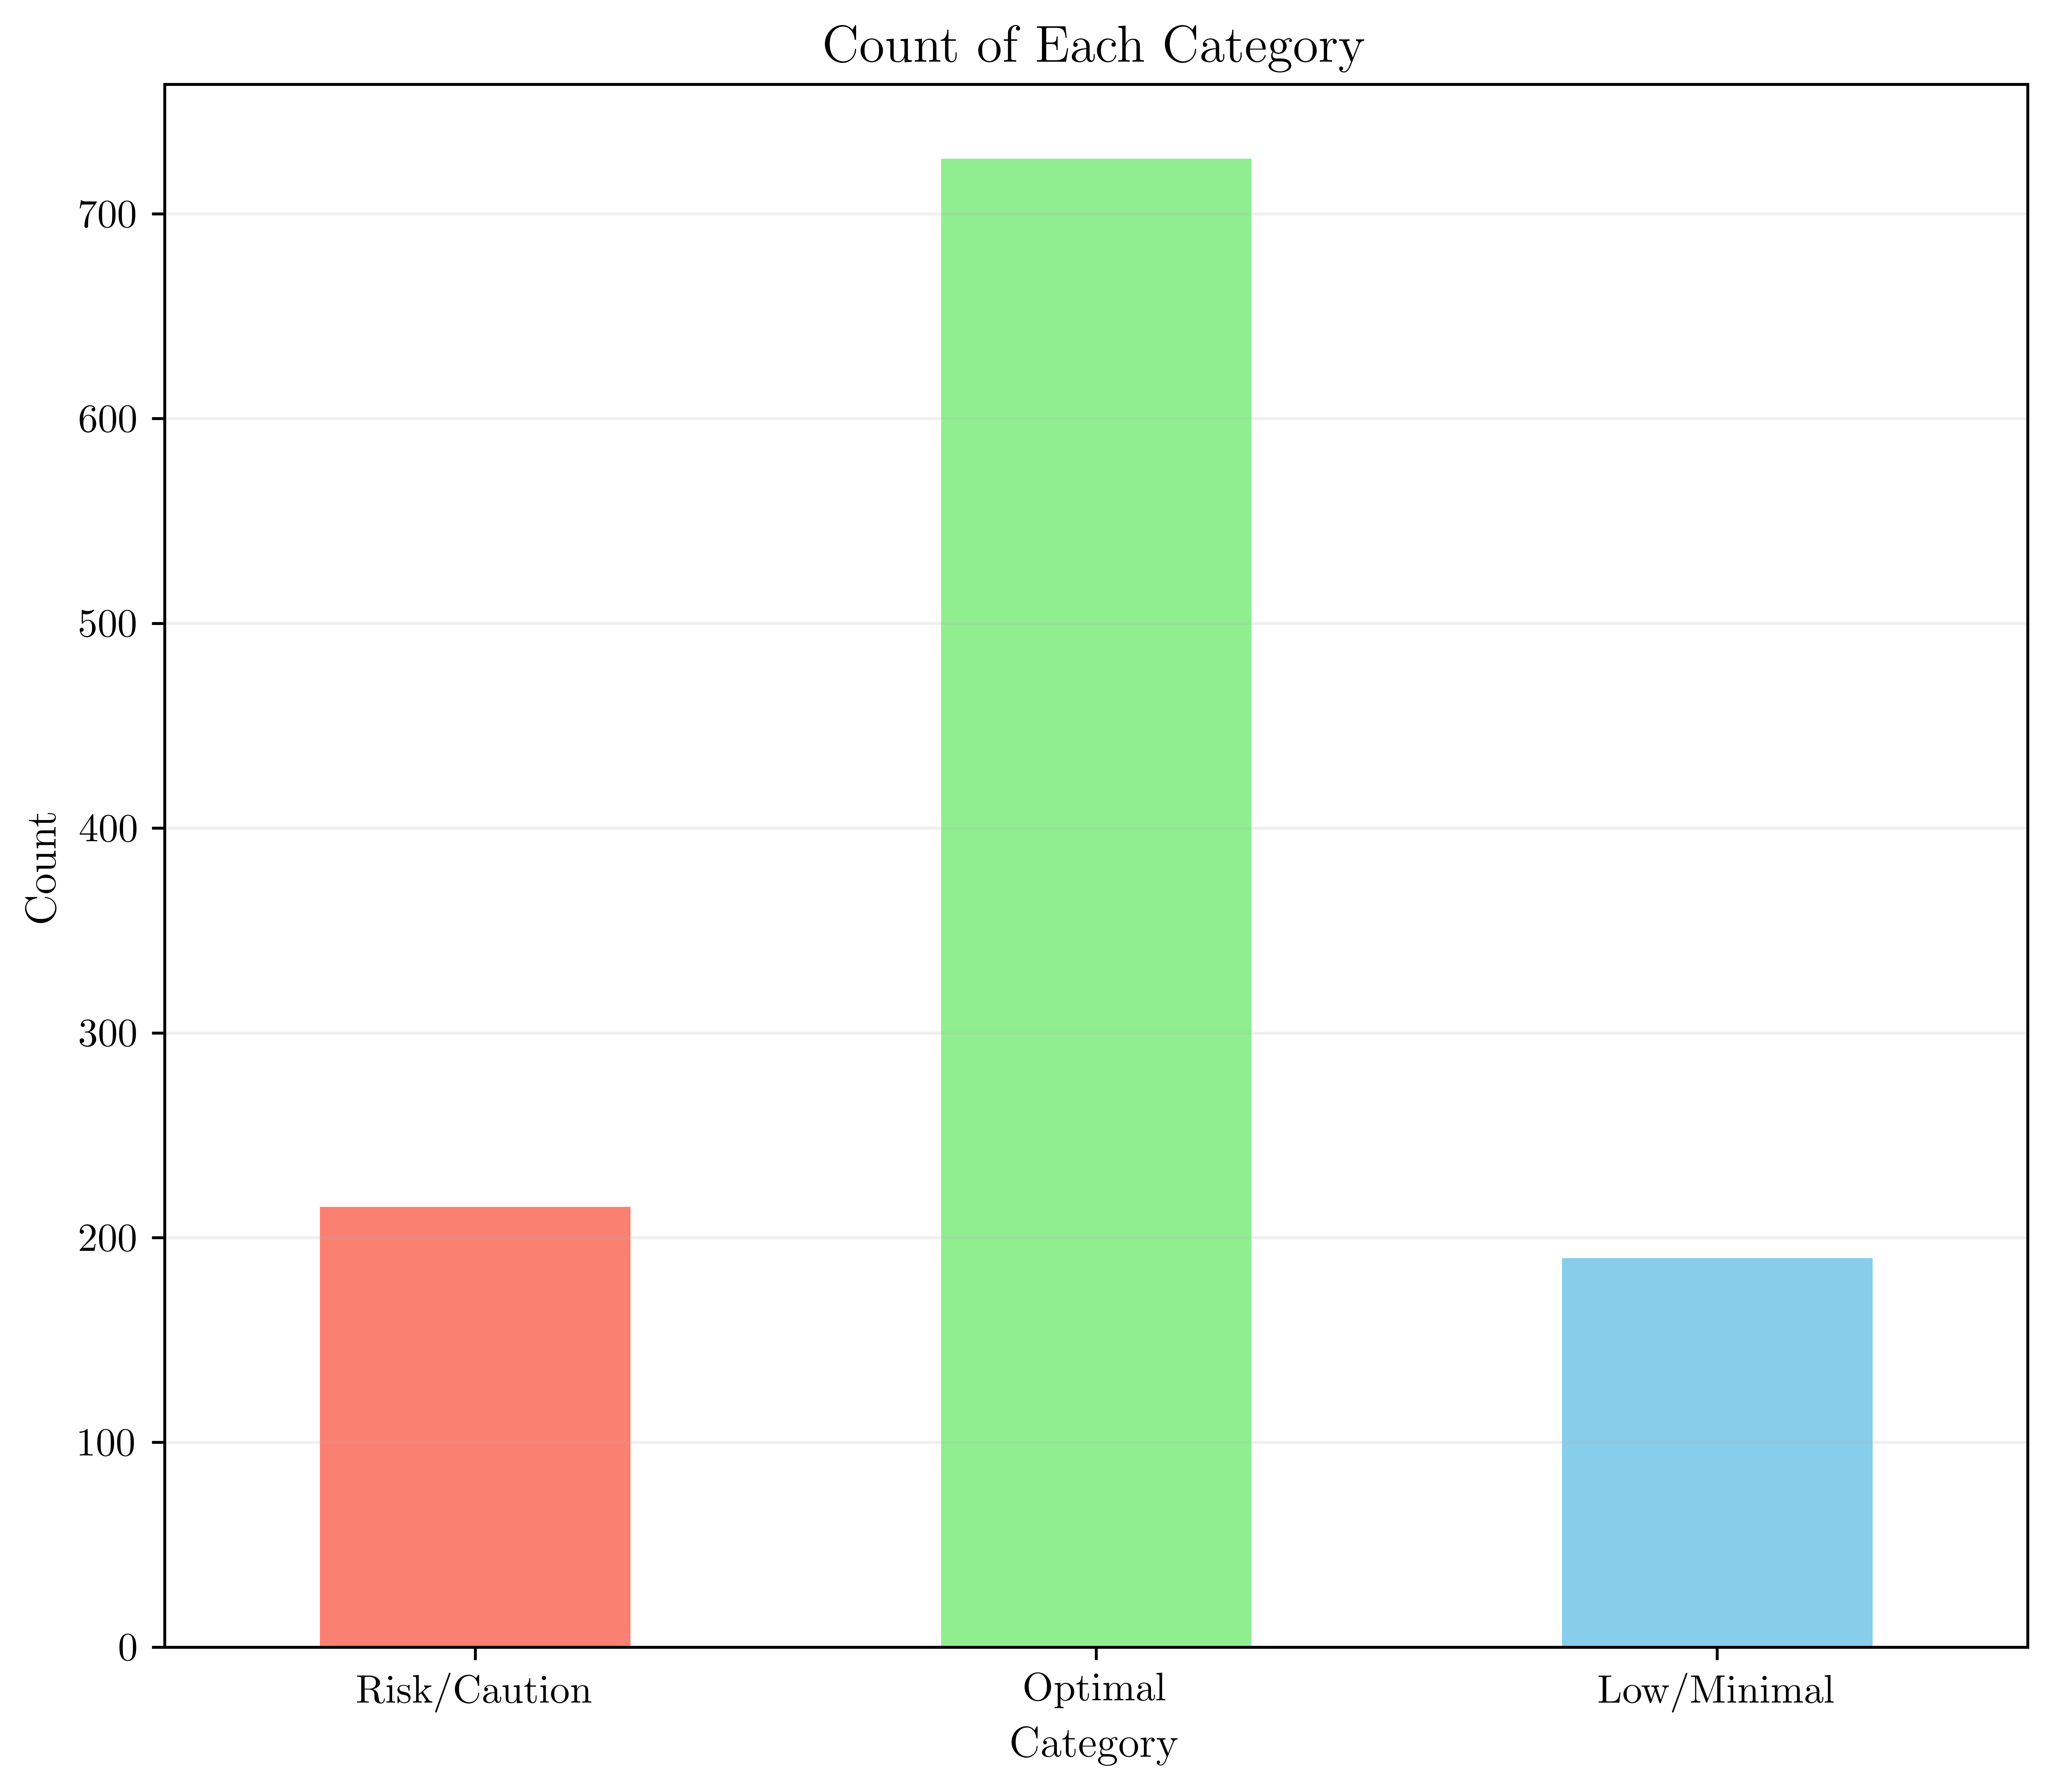
\includegraphics[width=1\linewidth]{assets/distribution_FatigInd(0).png}
    \caption{Bar plot of the new classes, once 'Caution' and 'Risk' are combined into one.}
    \label{histClasses}
\end{figure}

At this stage, we opted to under sample our dataset to the number of observations of 'Risk/Caution', and over sample the observations in 'Low/Minimal', by imputing random samples from the pool of observations of 'Low/Minimal', ending up with 213 observations per class (regardless of gender). The use of SMOTE in this scenario would give continuous classes for our features, which wouldn't yield any physical meaning.

To assess how the different features vary among them and in relation to the target, we computed the correlation matrix as seen in Figure \ref{fig:correlationMatrix}.

\begin{figure}[H]
    \centering
    \includegraphics[width=1\linewidth]{assets/correlation_matrix.png}
    \caption{Correlation matrix for all possible features considered for the models.}
    \label{fig:correlationMatrix}
\end{figure}

From the corr matrix it was possible to exclude several of the features, which was verified by how the classes are distributed across the scales for each feature. Figure \ref{classdist_feat} illustrates a proper and poor example of class distribution for the given features.

\begin{figure}[H]
    \centering
    \begin{subfigure}[1]{\linewidth}
        \centering
        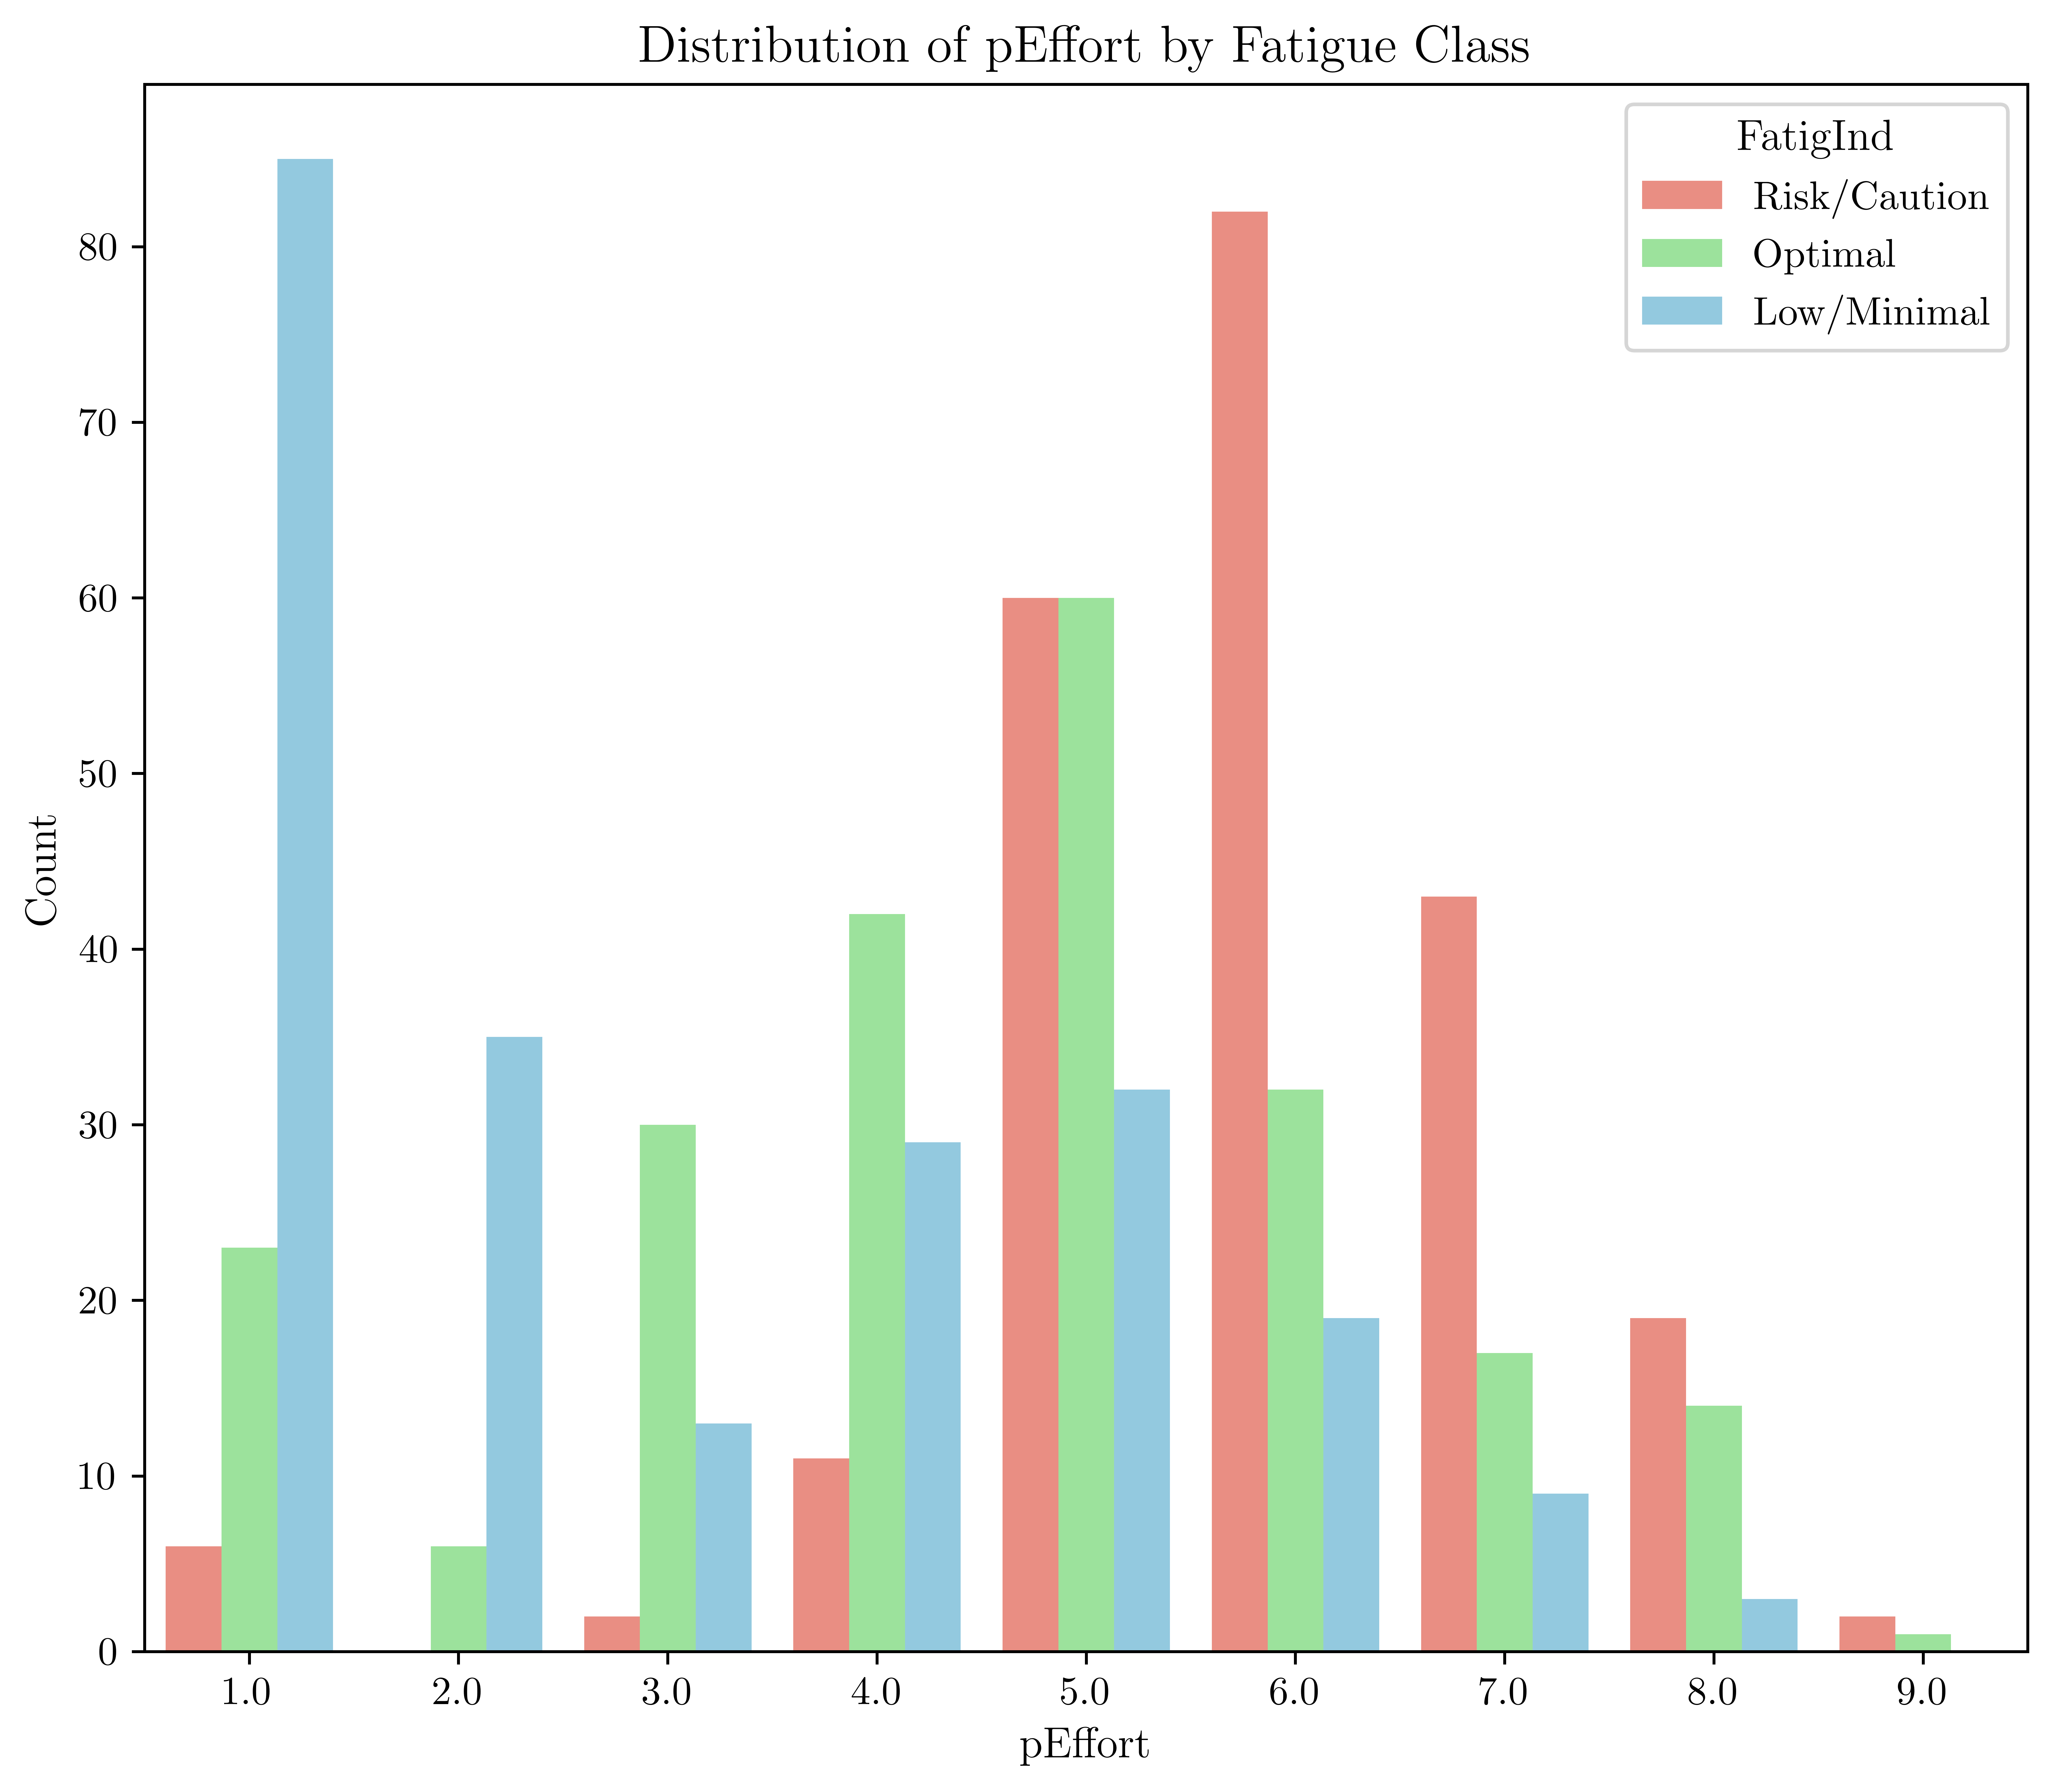
\includegraphics[width=\linewidth]{assets/distribution_pEffort.png}
        \caption{Distribution of perceived effort across classes.}
        \label{fig:subfig-a}
    \end{subfigure}
    
    \vspace{0.5cm}

    \begin{subfigure}[2]{\linewidth}
        \centering
        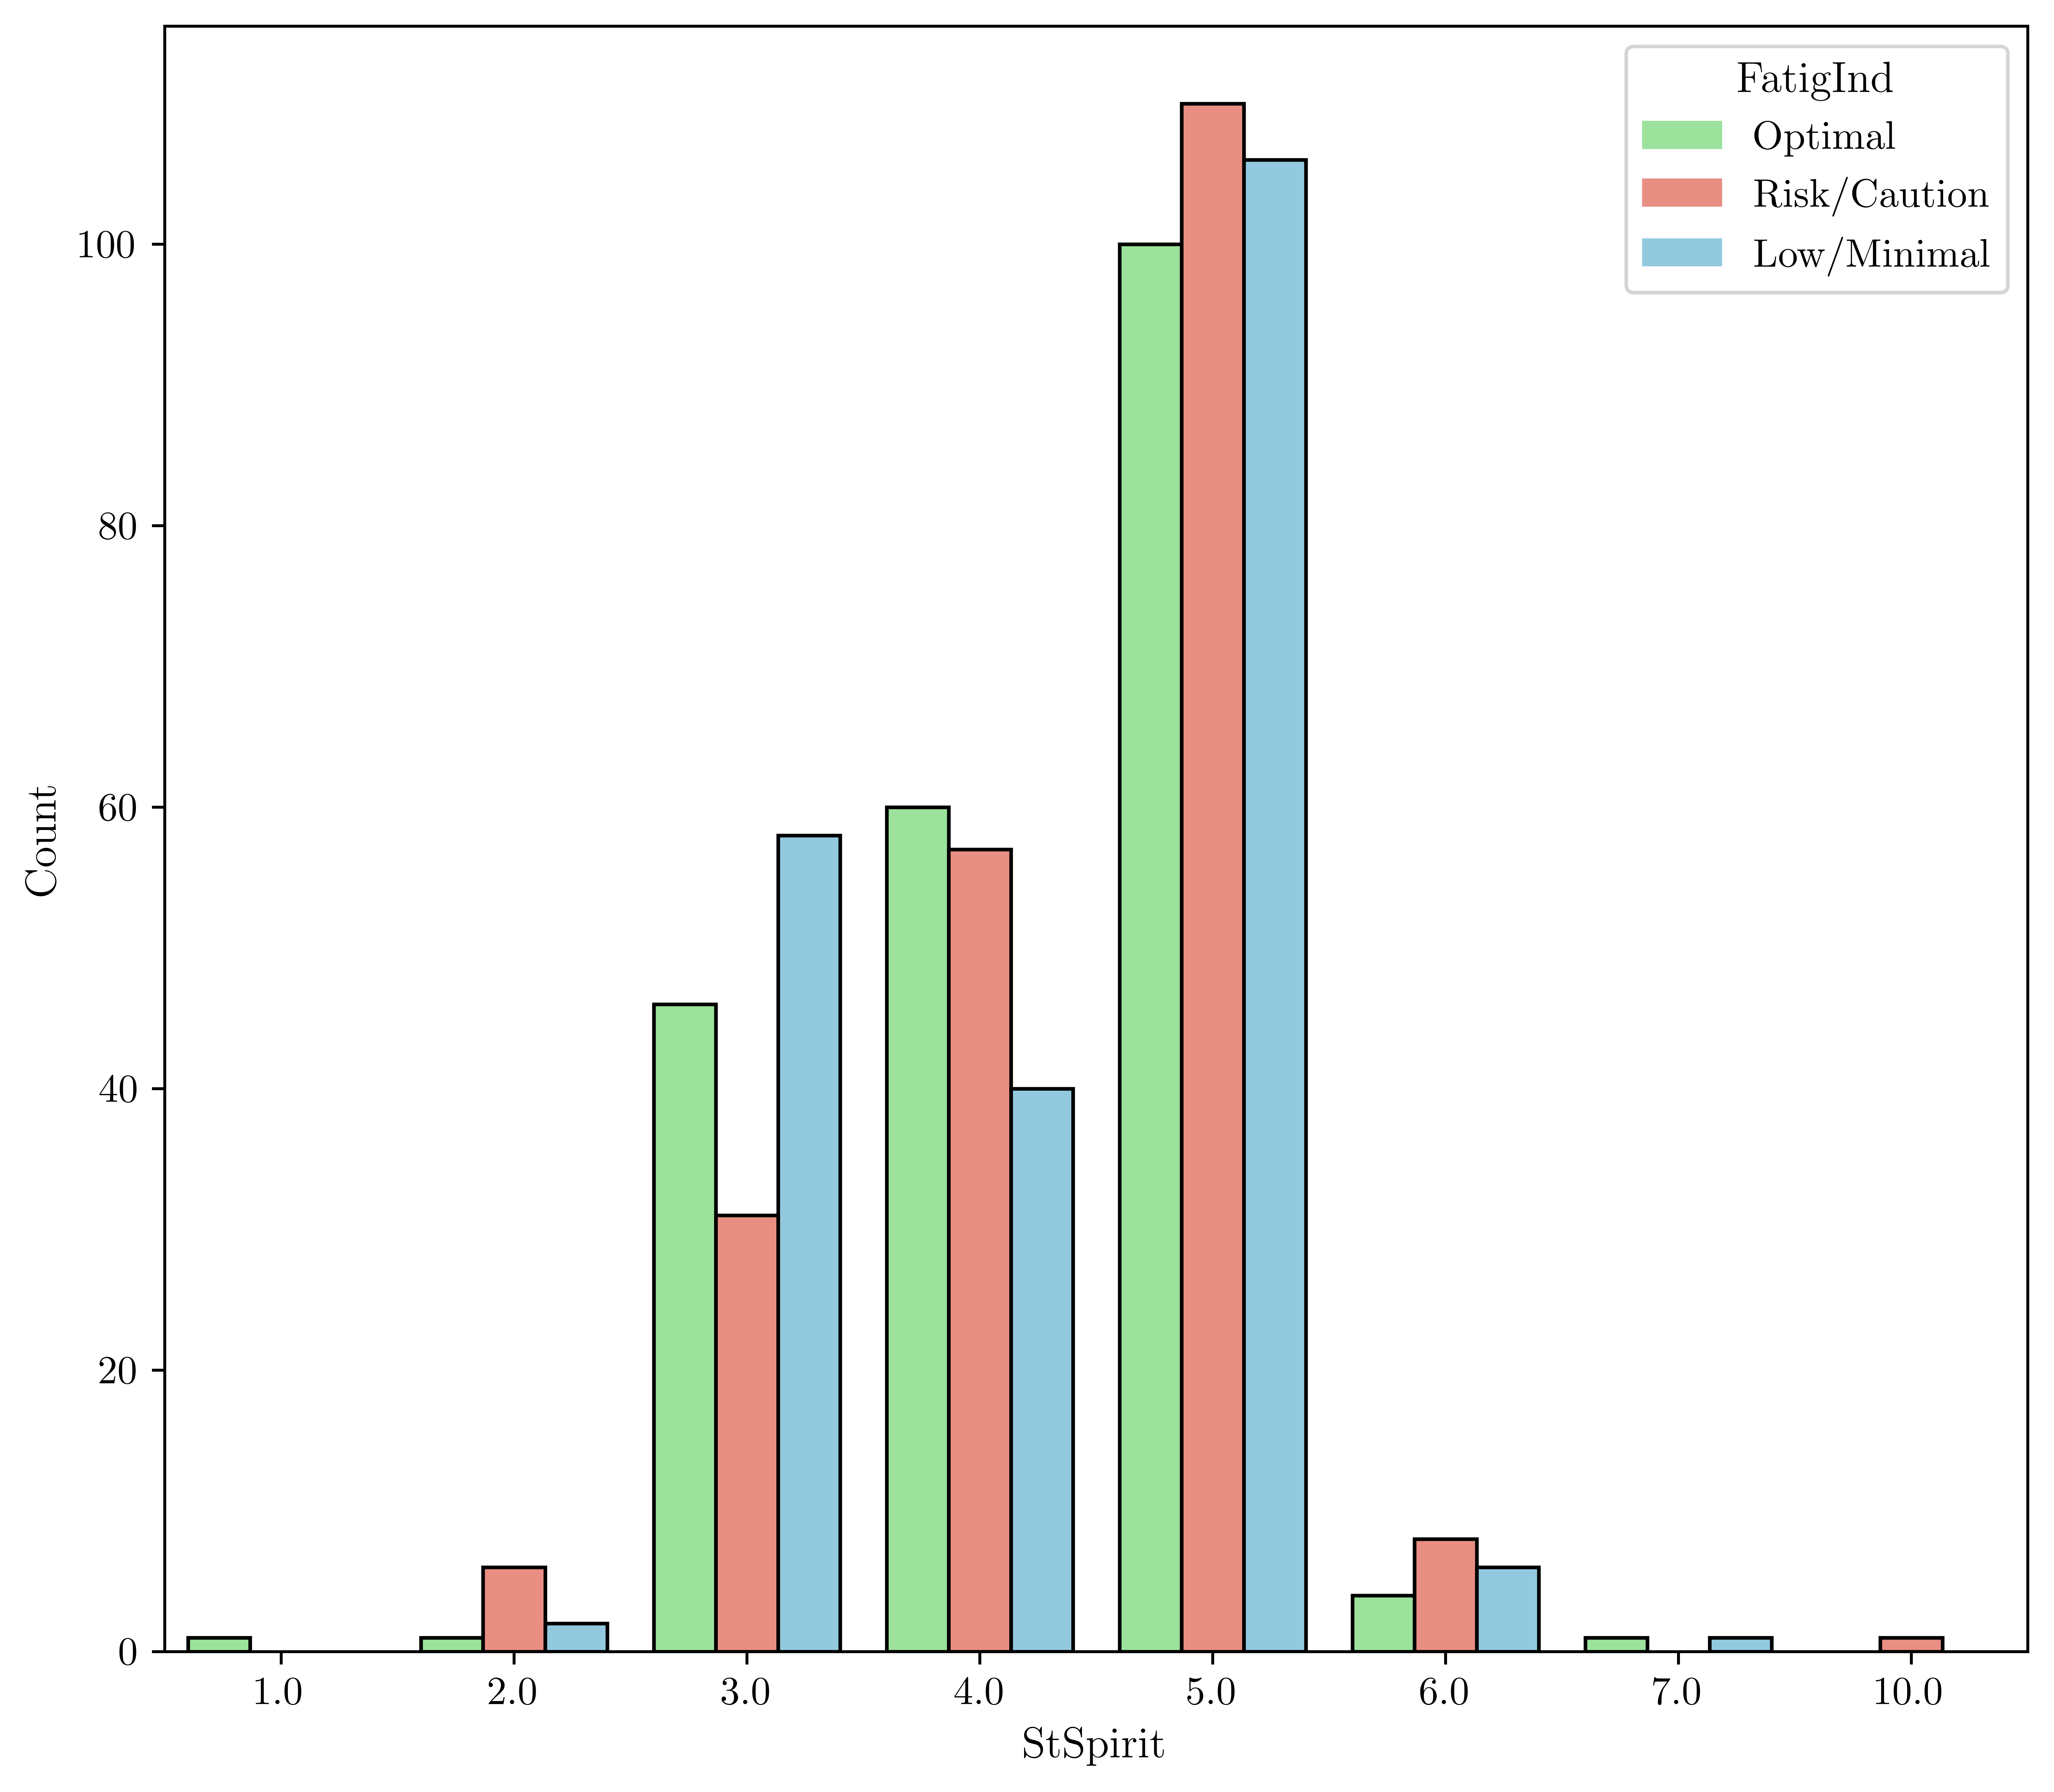
\includegraphics[width=\linewidth]{assets/distribution_StSpirit.png}
        \caption{Distribution of state spirit across classes.}
        \label{fig:subfig-b}
    \end{subfigure}
    
    \caption{Class distributions across different metrics: (a) perceived effort, (b) state spirit.}
    \label{classdist_feat}
\end{figure}

Considering that the weights used in the coach's original estimation of fatigue were identical regardless of sex, we performed some simple models in order to decide if it would be necessary to split it. We could verify that gender didn't have a significant impact in model performance, so we opted to use it as a feature. 

Figure \ref{fatig_Ff} illustrates the periodicity of higher training loads and subsequent lower intensity periods. It is important to refer that once the two higher intensity classes were combined the loss of granularity of how fatigue changes throughout the season is evident.  
\begin{figure}[H]
    \centering
    \includegraphics[width=1\linewidth]{assets/distribution_FatigInd(F_f).png}
    \caption{Daily fatigue trends for athlete F\_f.}
    \label{fatig_Ff}
\end{figure}

In order to keep the time series nature of training, increase and decrease of training intensity, and varying fatigue with training we included exponentially weighted moving averages (EWMA) \cite{Williams17}.

This way memory is introduced in our model, and allow to consider the decay in the weights of events further away from any given day. The mathematical expression used to calculate EWMA for each selected feature is,
\begin{equation*}
    \text{EWMA}_{\text{today}} = \text{Feature}_{\text{today}} \cdot \lambda_a + (1 - \lambda_a) \cdot \text{EWMA}_{\text{yesterday}}
\end{equation*}
where $\lambda_a$ is a value between 0 and 1 that represents the degree of decay, with higher values discounting older observations at a faster rate. The $\lambda_a$ is given by:
\begin{equation*}
    \lambda_a = \frac{2}{N + 1}
\end{equation*} 

At this point it was possible to select the most relevant features for modeling: (\textit{pEffort}), (\textit{uaI}), (\textit{SleepInd}), (\textit{Sex\_F}), (\textit{pEffort(MA6)}), (\textit{SleepInd(MA6)}), (\textit{uaI(MA6)}), (\textit{Appetite(MA6)}).

%\newpage
\section{Classification Models}

In this section the results for the three machine learning models are presented and detailed in equal fashion, to facilitity the discussion and interpretation in the next section. As was mentioned in the methodology, the modeling approach was the same for all, and here the training dataset results are presented first, followed by the test dataset results.

\section{Logistic Regression}

The logistic regression model was developed by setting different ranges for the hyperparameters, with $C$, the inverse of the regularization parameter, varying between $0.01$ and $300$, and allowing the selection of different cost functions ($L1$, $L2$, or none). Due to the suboptimal performance of the 'Optimal' class in terms of precision, we also decided to adjust the class weights for 'Risk/Caution' and 'Low/Minimal' within a range of 0.1 to 2. The resulting model with the highest accuracy is illustrated in Figure~\ref{logregWt}.

\begin{figure}[H]
    \centering
    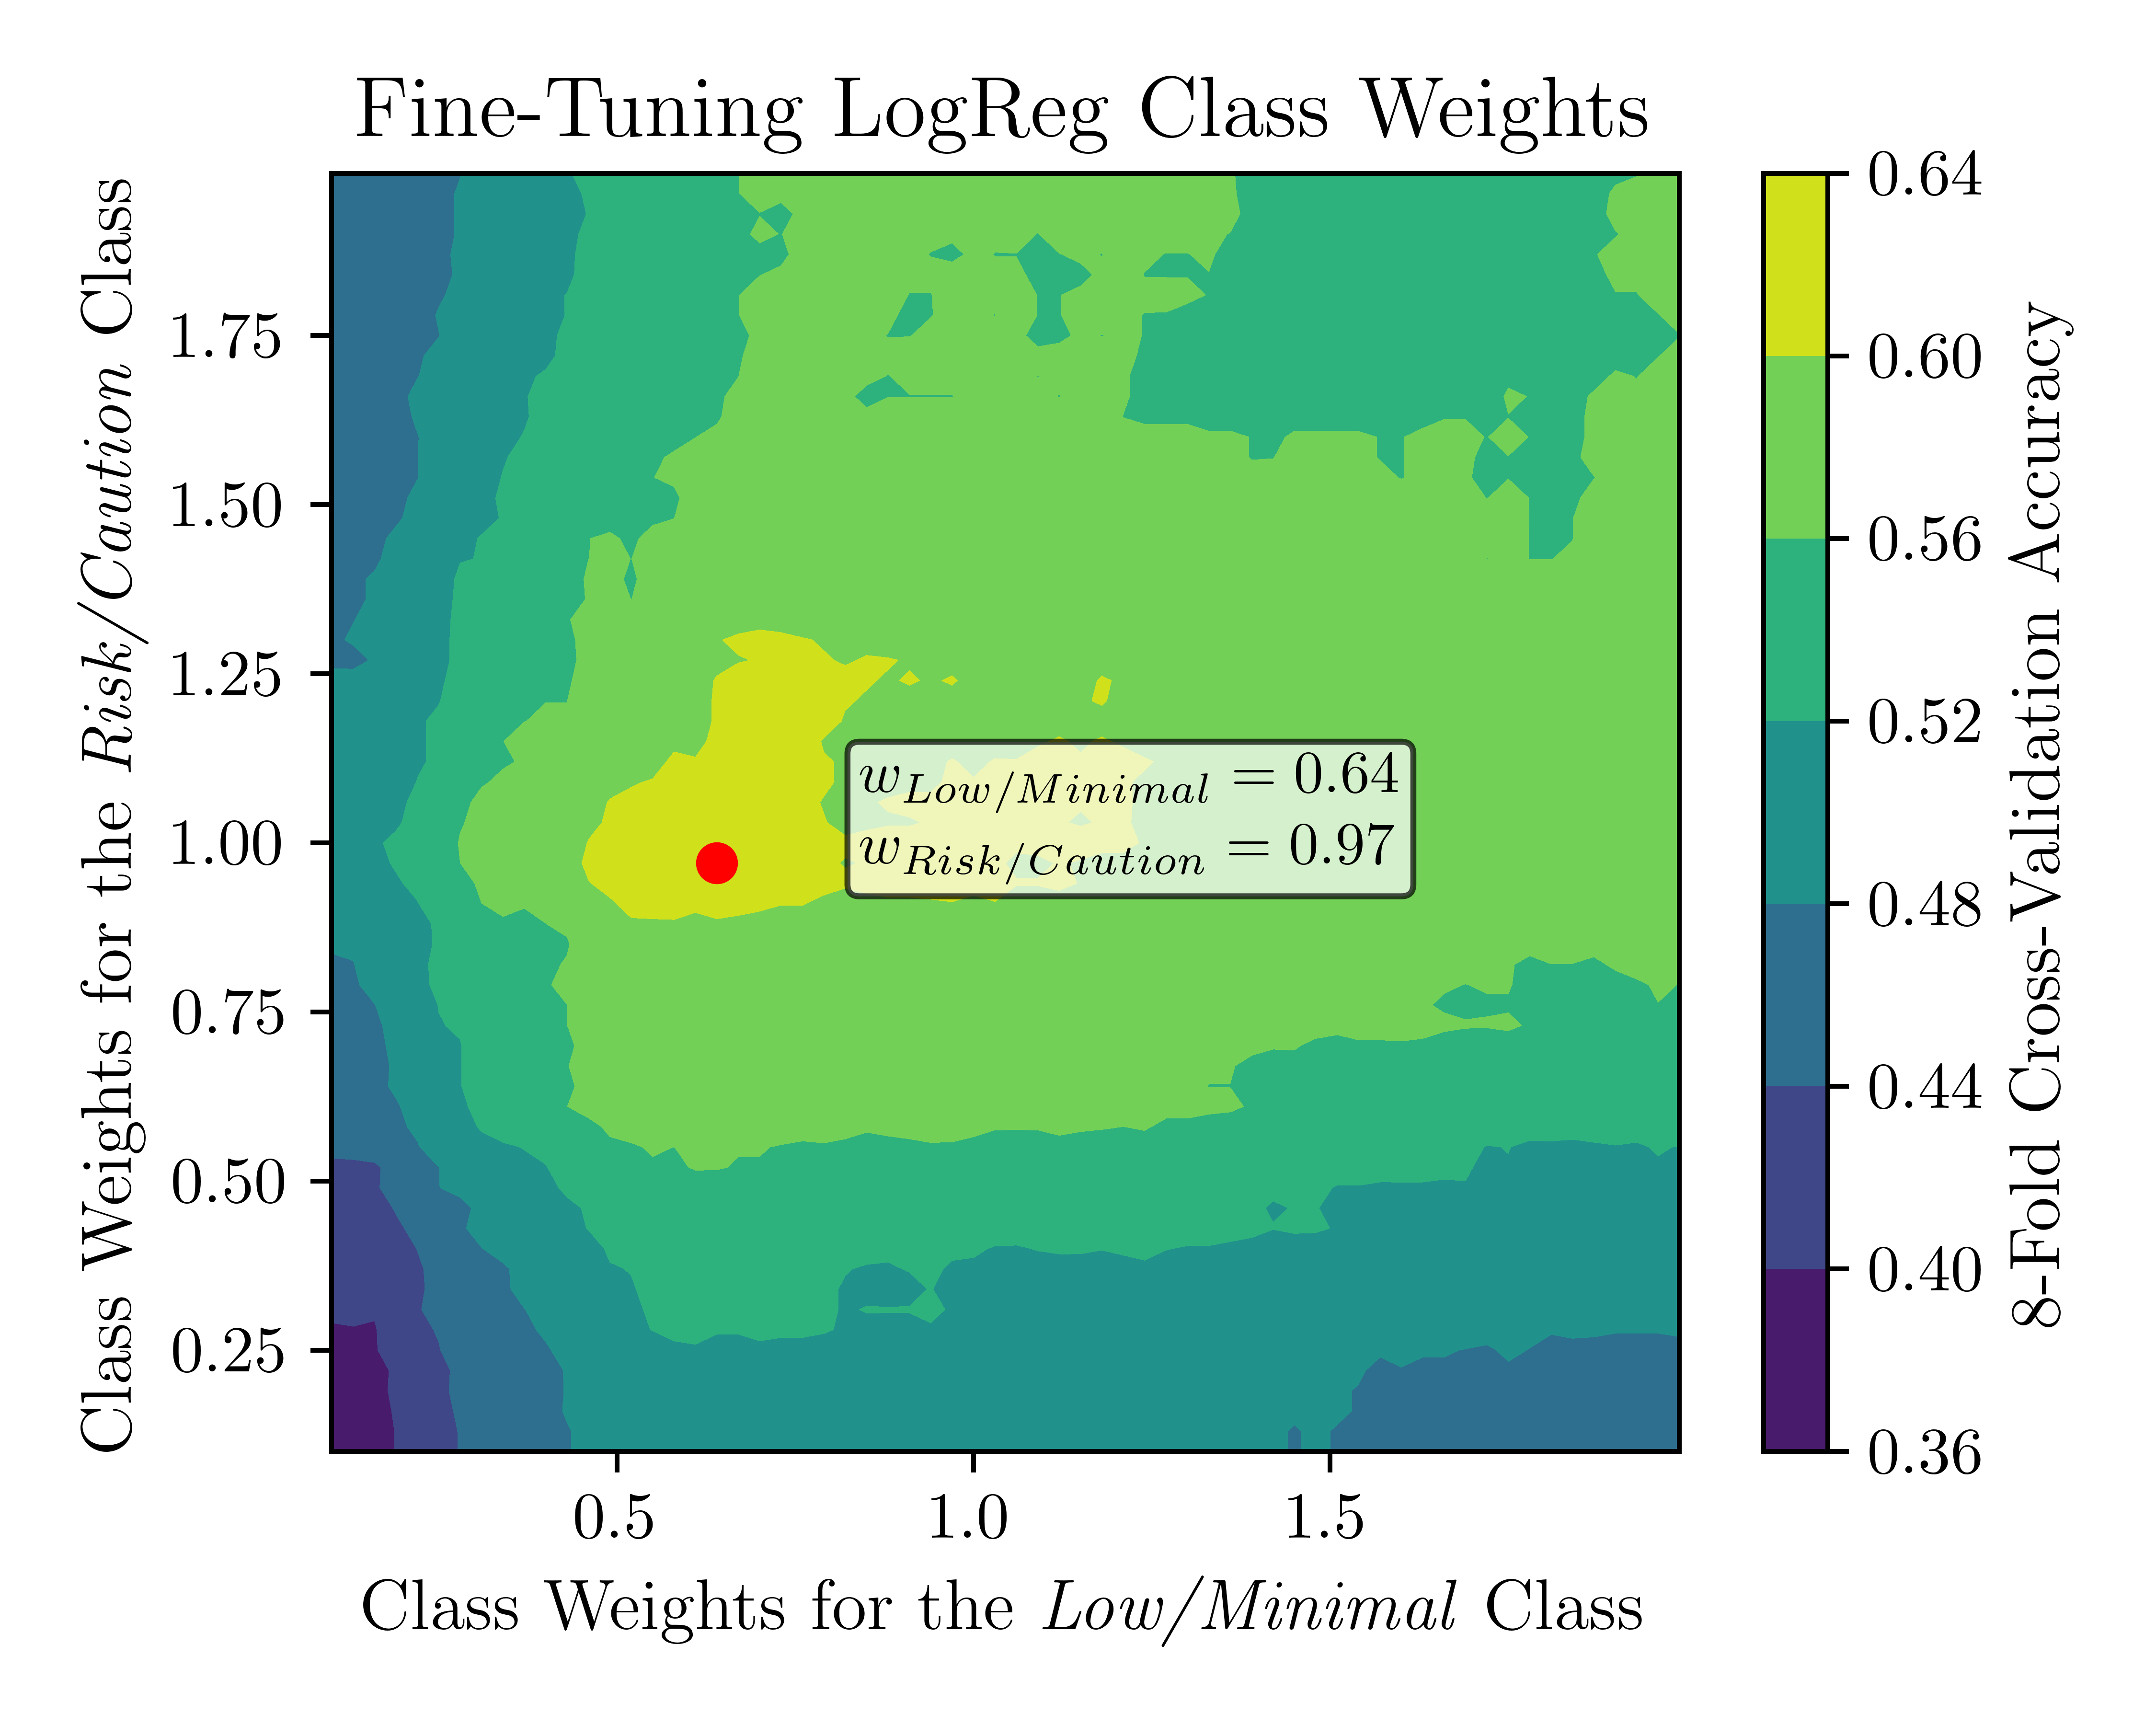
\includegraphics[width=1\linewidth]{assets/LOGR_class_weights.png}
    \caption{Effect of the 'Risk/Caution' and 'Low/Minimal' classes weight on LogReg model accuracy.}
    \label{logregWt}
\end{figure}

Since the highest accuracy was achieved with class weights of 0.64 for 'Low/Minimal' and 0.97 for 'Risk/Caution', these values were selected, while the original weight for the 'Optimal' class was retained. These weight values were applied consistently across both the training and test datasets. For model optimization, the remaining hyperparameters were set to $C \approx 2.13$, the cost function was $L1$ (Lasso regularization) and the solver used was $SAGA$ (Stochastic Average Gradient Augmented).

% Poderá ser útil comentar este solver, e que na verdade até pode não ser o mais indicado para o problema que estamos a resolver, mas foi o sugerido (tipicamente é indicado para grandes datasets, e que tenham valores em falta e assim).

The learning curve shown in Figure \ref{cf_train_LogReg} illustrates the relationship between the training set size and the performance of the adjusted model, providing valuable insight to assess the model's behavior in terms of overfitting or underfitting. In this case, the learning curves from the training and the cross-validation converge after the largest training set size of 450, with no signs of over fitting.

\begin{figure}[H]
    \centering
    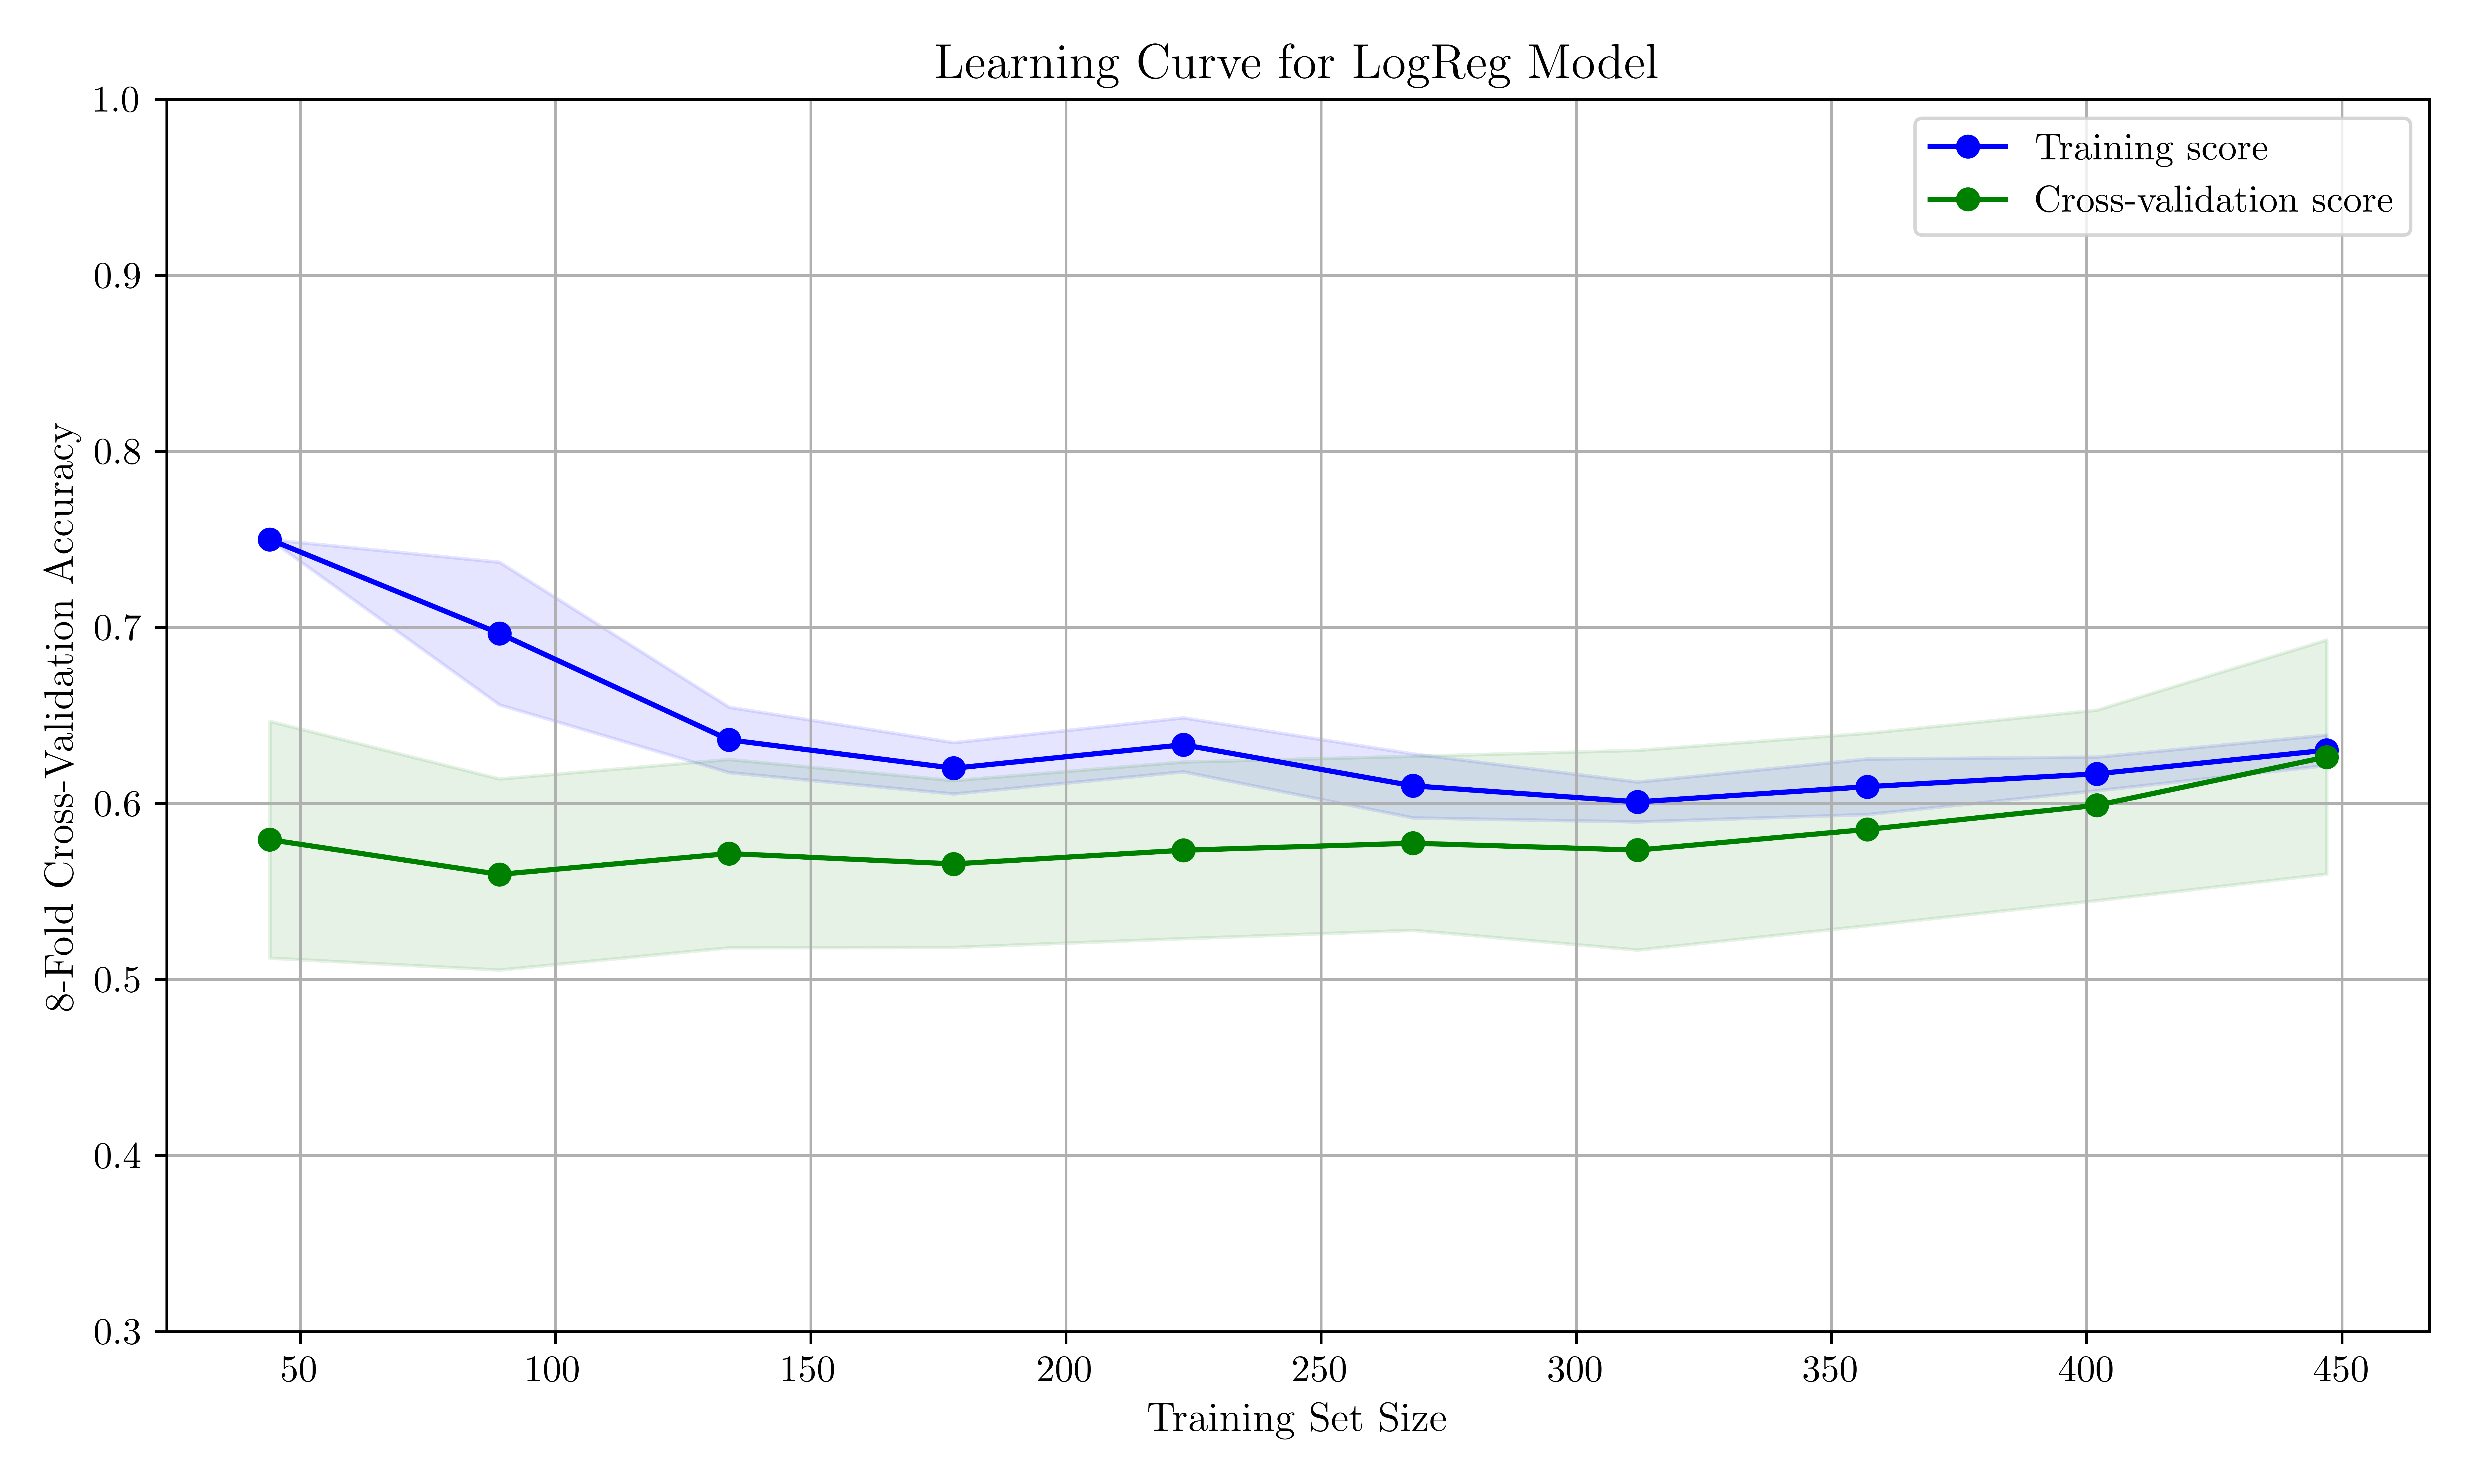
\includegraphics[width=1\linewidth]{assets/LOGR_lercurve.png}
    \caption{LogReg model performance using learning curve representation across varying training data sizes.}
    \label{lcLogReg}
\end{figure}

\begin{figure}[H]
    \centering
    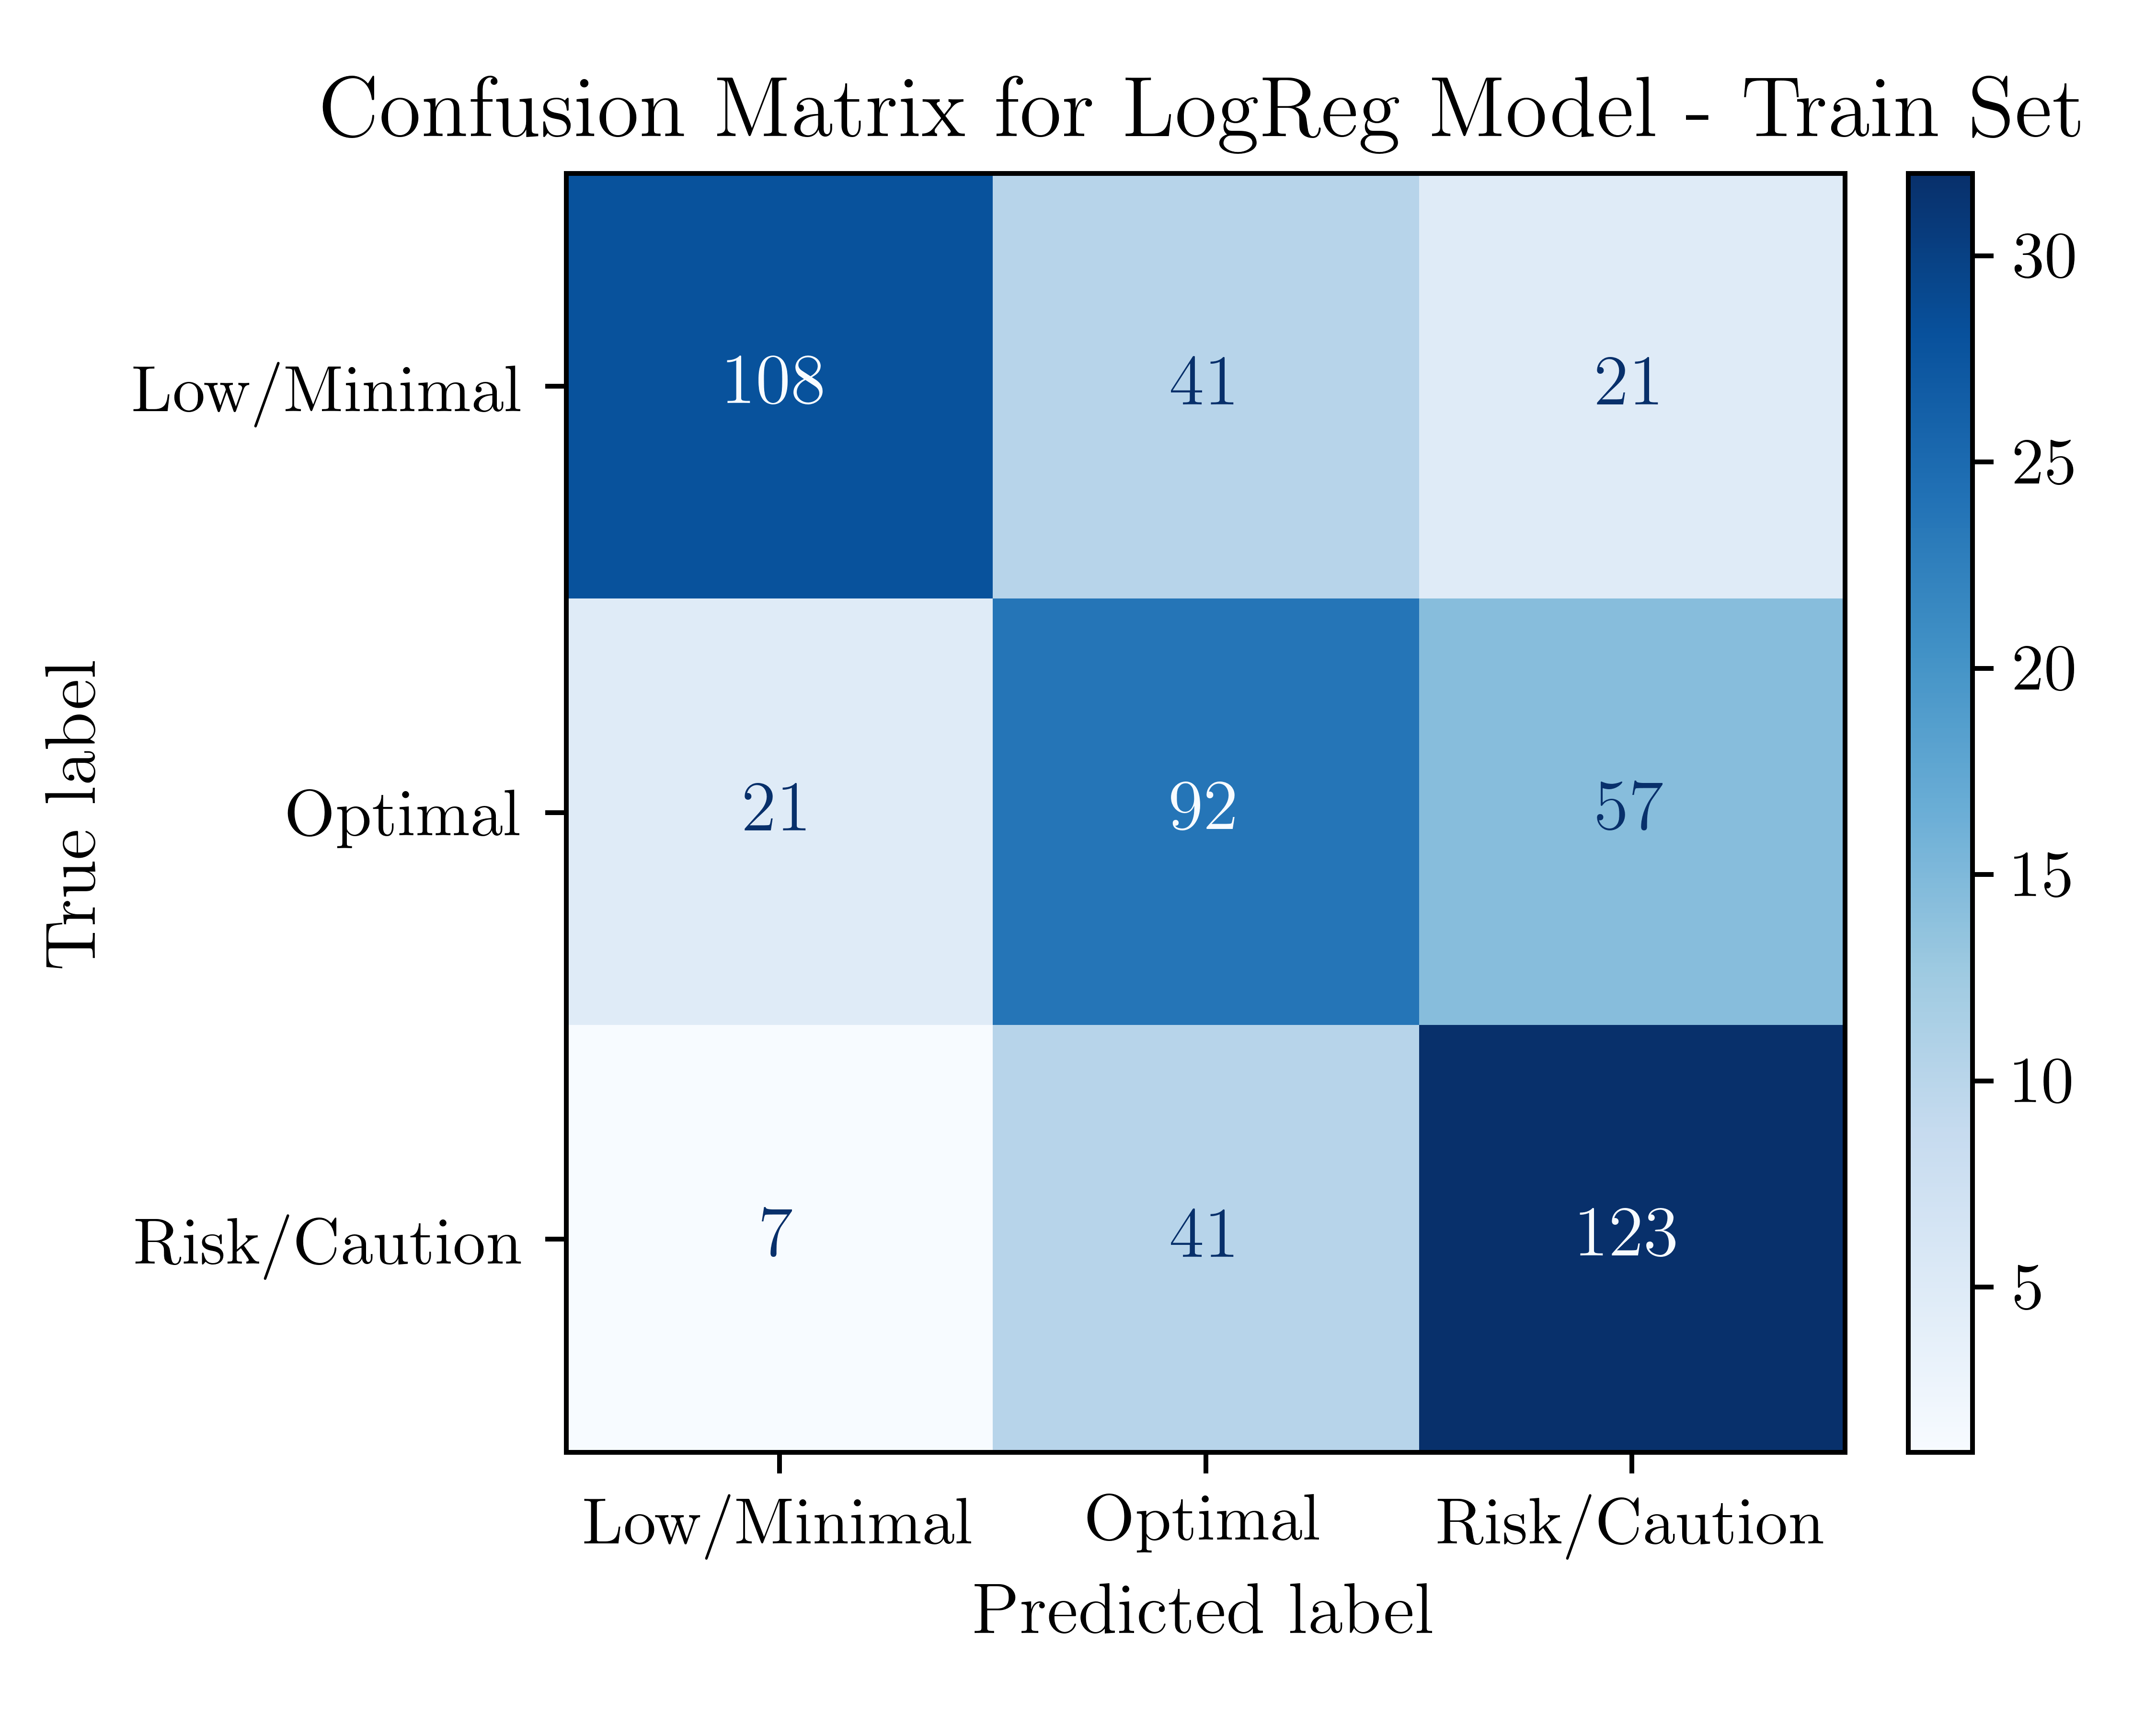
\includegraphics[width=1\linewidth]{assets/LOGR_confmatTrain.png}
    \caption{Confusion matrix for the training data of LogReg model.}
    \label{cf_train_LogReg}
\end{figure}

\begin{table}[H]
\centering
\caption{Classification report for LogReg model performance evaluation on training data.}
\label{crTrainLogReg}
\begin{tabular}{lcccccc}
\toprule
\textbf{Class} & \textbf{Precision} & \textbf{Recall} & \textbf{F1-Score} & \textbf{Support} \\
\midrule
Low/Minimal & 0.79 & 0.64 & 0.71 & 170 \\
Optimal & 0.53 & 0.54 & 0.53 & 170 \\
Risk/Caution & 0.61 & 0.72 & 0.66 & 171 \\
\midrule
\textbf{Accuracy} &  &  & 0.63 & 511 \\
\textbf{Macro avg} & 0.64 & 0.63 & 0.63 & 511 \\
\textbf{Weighted avg} & 0.64 & 0.63 & 0.63 & 511 \\
\bottomrule
\end{tabular}
\end{table}

\begin{figure}[H]
    \centering
    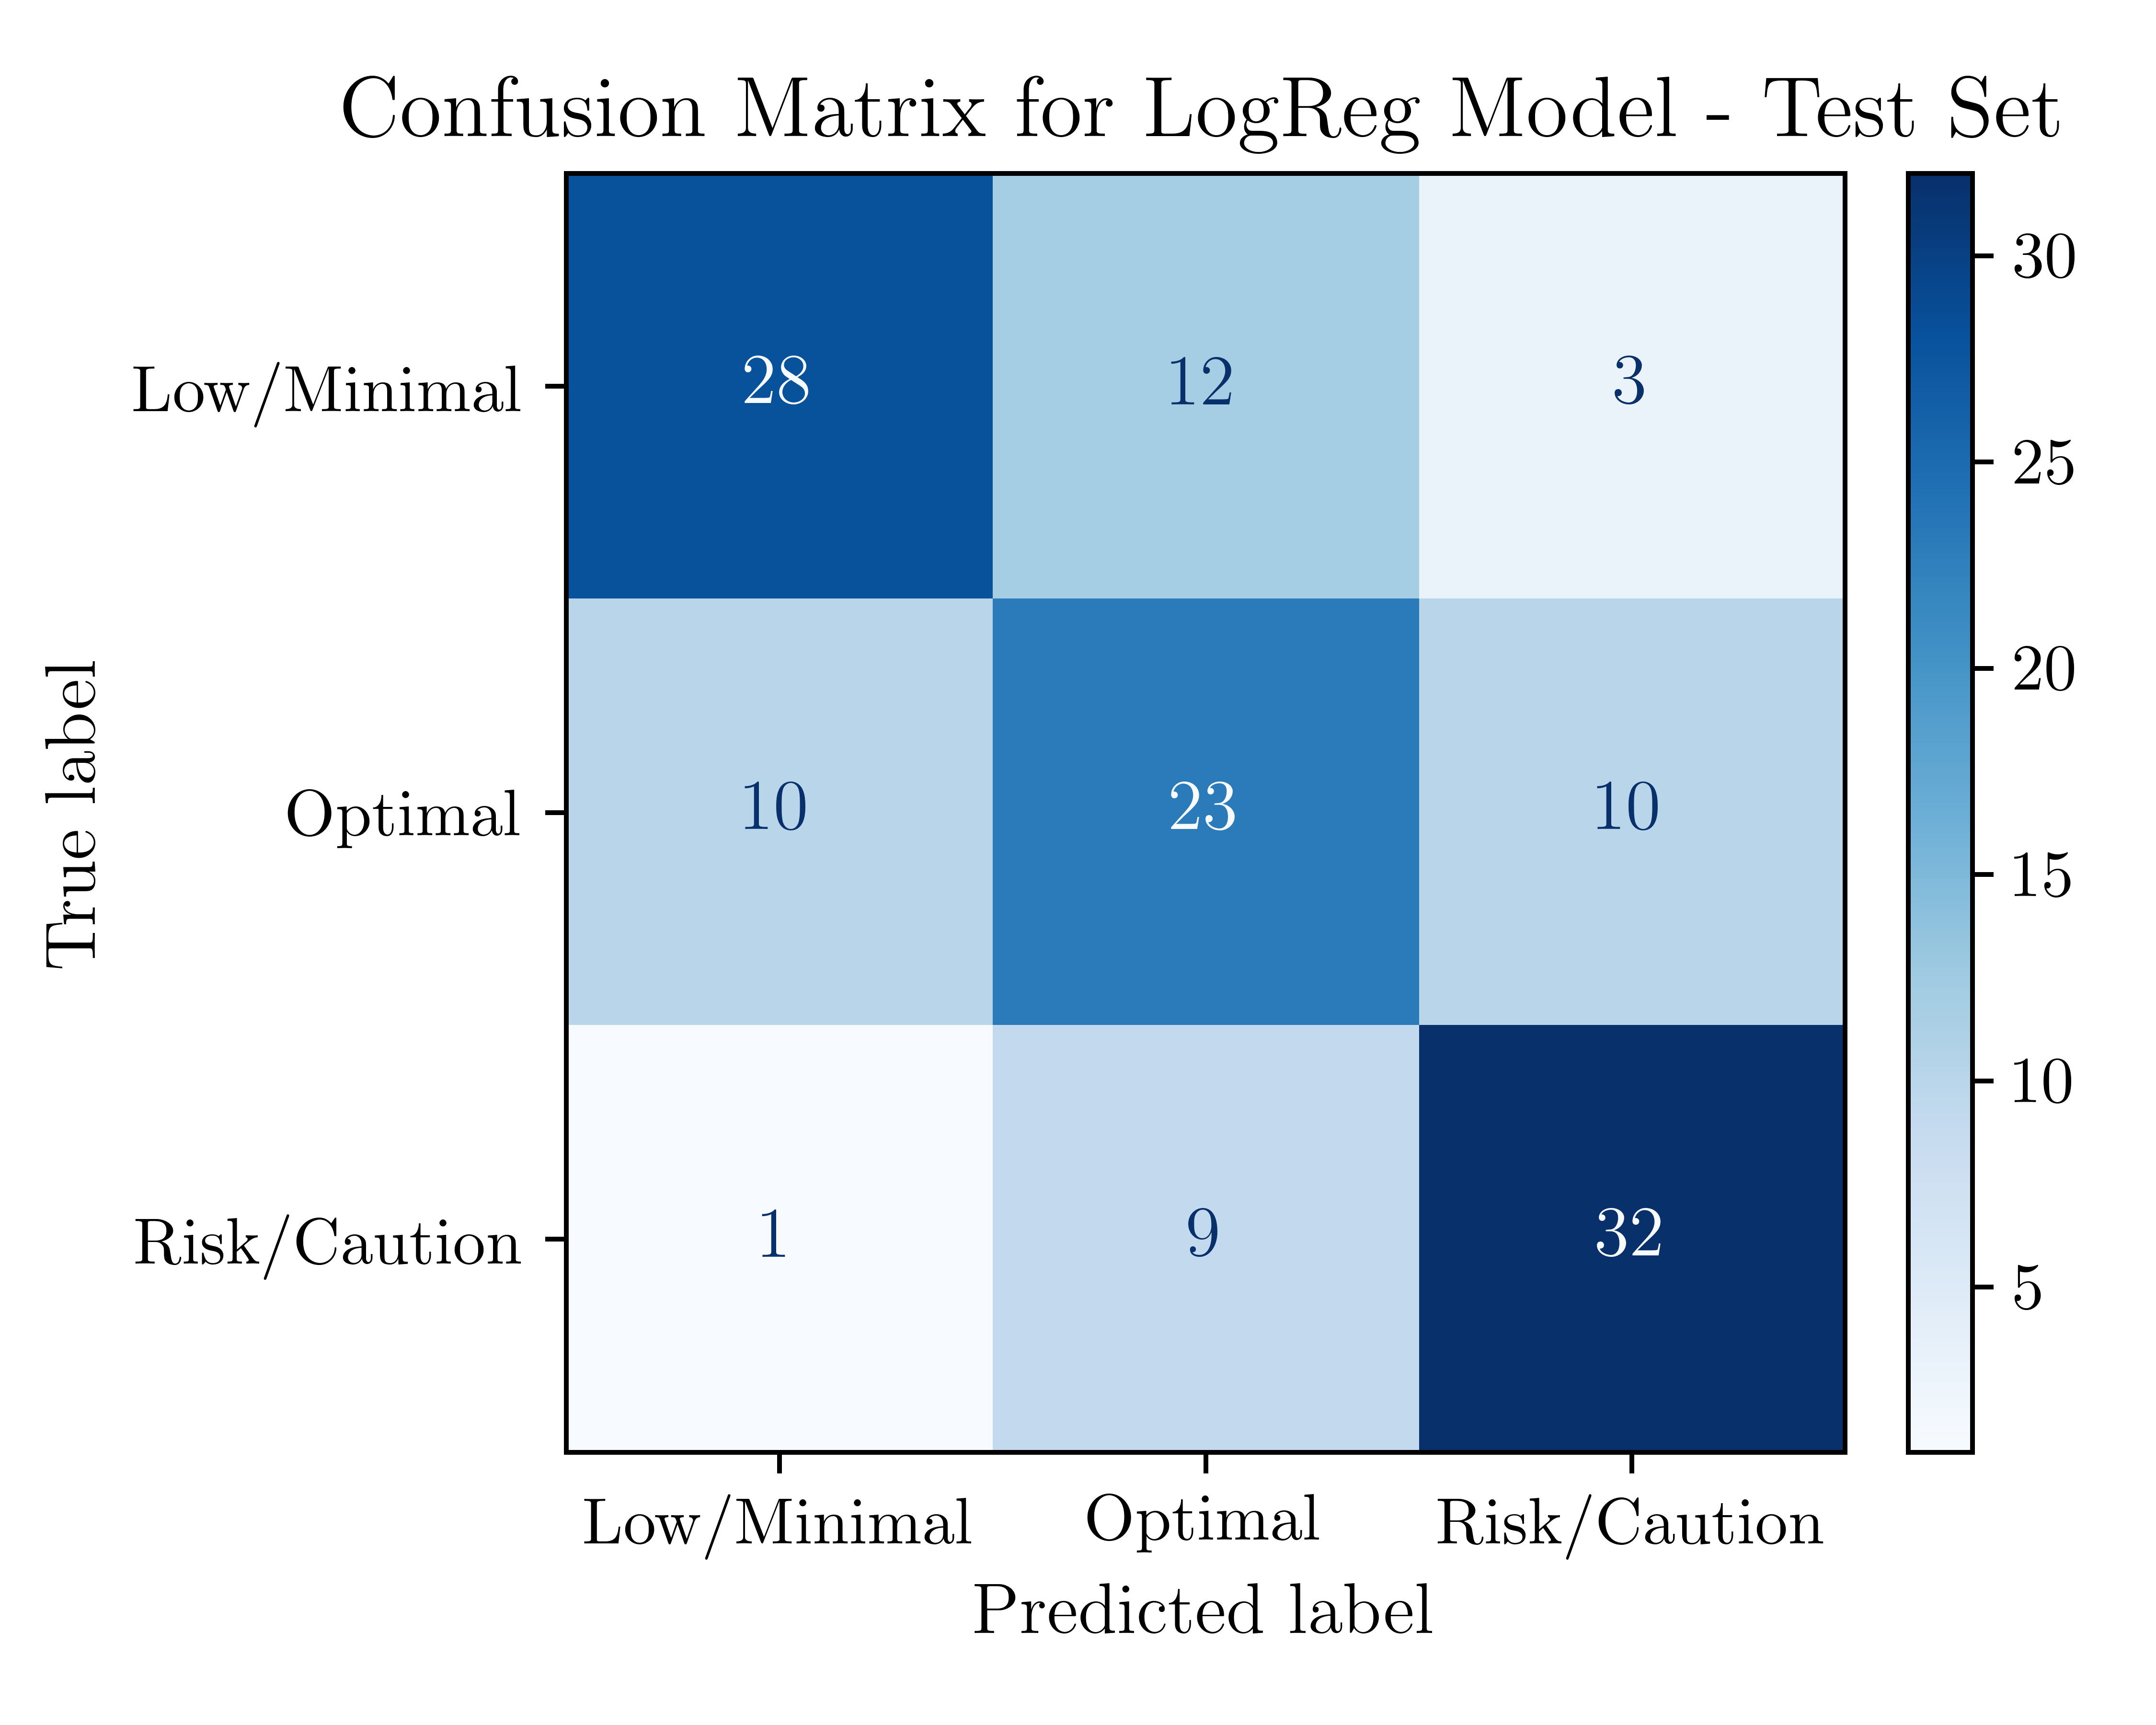
\includegraphics[width=1\linewidth]{assets/LOGR_confmatTest.png}
    \caption{Confusion matrix for the test data of LogReg model.}
    \label{cm_Test_LogReg}
\end{figure}

\begin{table}[H]
\centering
\caption{Classification report for LogReg model performance evaluation on test data.}
\label{crTestLogREg}
\begin{tabular}{lcccccc}
\toprule
\textbf{Class} & \textbf{Precision} & \textbf{Recall} & \textbf{F1-Score} & \textbf{Support} \\
\midrule
Low/Minimal & 0.72 & 0.65 & 0.68 & 43 \\
Optimal & 0.52 & 0.52 & 0.53 & 43 \\
Risk/Caution & 0.71 & 0.76 & 0.74 & 42 \\
\midrule
\textbf{Accuracy} &  &  & 0.65 & 128 \\
\textbf{Macro avg} & 0.65 & 0.65 & 0.65 & 128 \\
\textbf{Weighted avg} & 0.65 & 0.65 & 0.65 & 128 \\
\bottomrule
\end{tabular}
\end{table}

Tendo em conta as matrizes de confusão relativamente aos dados de treino (Fig. \ref{cf_train_LogReg}) e de teste (fig. \ref{cm_Test_LogReg}), estas permitem-nos perceber how well the model predicts the true labels compared to the actual labels. Neste caso, possível verificar algumas semelhanças entre as duas, nomeadamente o melhor desempenho na classificação das classes extremas ('Low/Minimal' e 'Risk/Caution') face à classe 'Optimal', apesar dos pesos dados, (mas sempre é melhor do q era antes no modelo sem os pesos).

Quanto aos classifciation report, estes pertitem-nos comparar o desempenho dos dados de treino (table \ref{crTrainLogReg}) e de teste (table \ref{crTestLogREg}), de modo a ter insights sobre a possiblidade de haver ou não overfitting. Neste caso, ambos os class report apresentam resultados bastante semelhantes, pelo que hão levanta suspeitas sobre overfitting. para alem disso, tambem se verificam melhores resultados para as classes extremas e piores para o 'Optimal', o q já seria de esperar tendo em conta as matrizes de confusao.


\section{Support Vector Machine}

Given the increased complexity compared to LogReg, the support vector machine (SVM) model allows for manipulation of a larger number of hyperparameters, which consequently lead to longer computation times to achieve the best model. The hyperparameters used were Regularization Parameter (parameter that controls the penalty for misclassified training examples, i.e., cost function) ($C$), the Kernel Coefficient ($\gamma$), the kernel to be used, the highest degree possible (for a $poly$ kernel), and the value of the independent term (Coef$_0$), which controls the flexibility of the decision boundary \cite{svm24}. The ranges of possible values can be assessed in Table \ref{parametrosSVM}.

\begin{table}[H]
\centering
\caption{SVM model hyperparameters search space.}
\label{parametrosSVM}
\begin{tabular}{ll}
\toprule
\textbf{Hyperparameter} & \textbf{Possible Values} \\
\midrule
$C$ & $[0, 100]$ \\ 
$\gamma$ & \{scale, auto, $0.1$, $0.01$, $0.001$\} \\ 
Kernel & \{linear, rbf, poly, sigmoid\} \\ 
Degree & \{1, 2, 3\} \\ 
Coef$_0$ & $[-5, 5]$ \\
\bottomrule
\end{tabular}
\end{table}

As in the case for LogReg, an ideal class weight was estimated, however here only for 'Optimal' class, as it was the worst predicted class even at a training stage, with an equal split between 'Low/Minimal' and 'Risk/Caution'. É importante referir que estes pesos oq fazem é aumentar a penalização para classificacoes incorretas, nomedamente: $C_{class} \leftarrow C \times w_{class}$ \cite{svm24}.

\begin{figure}[H]
    \centering
    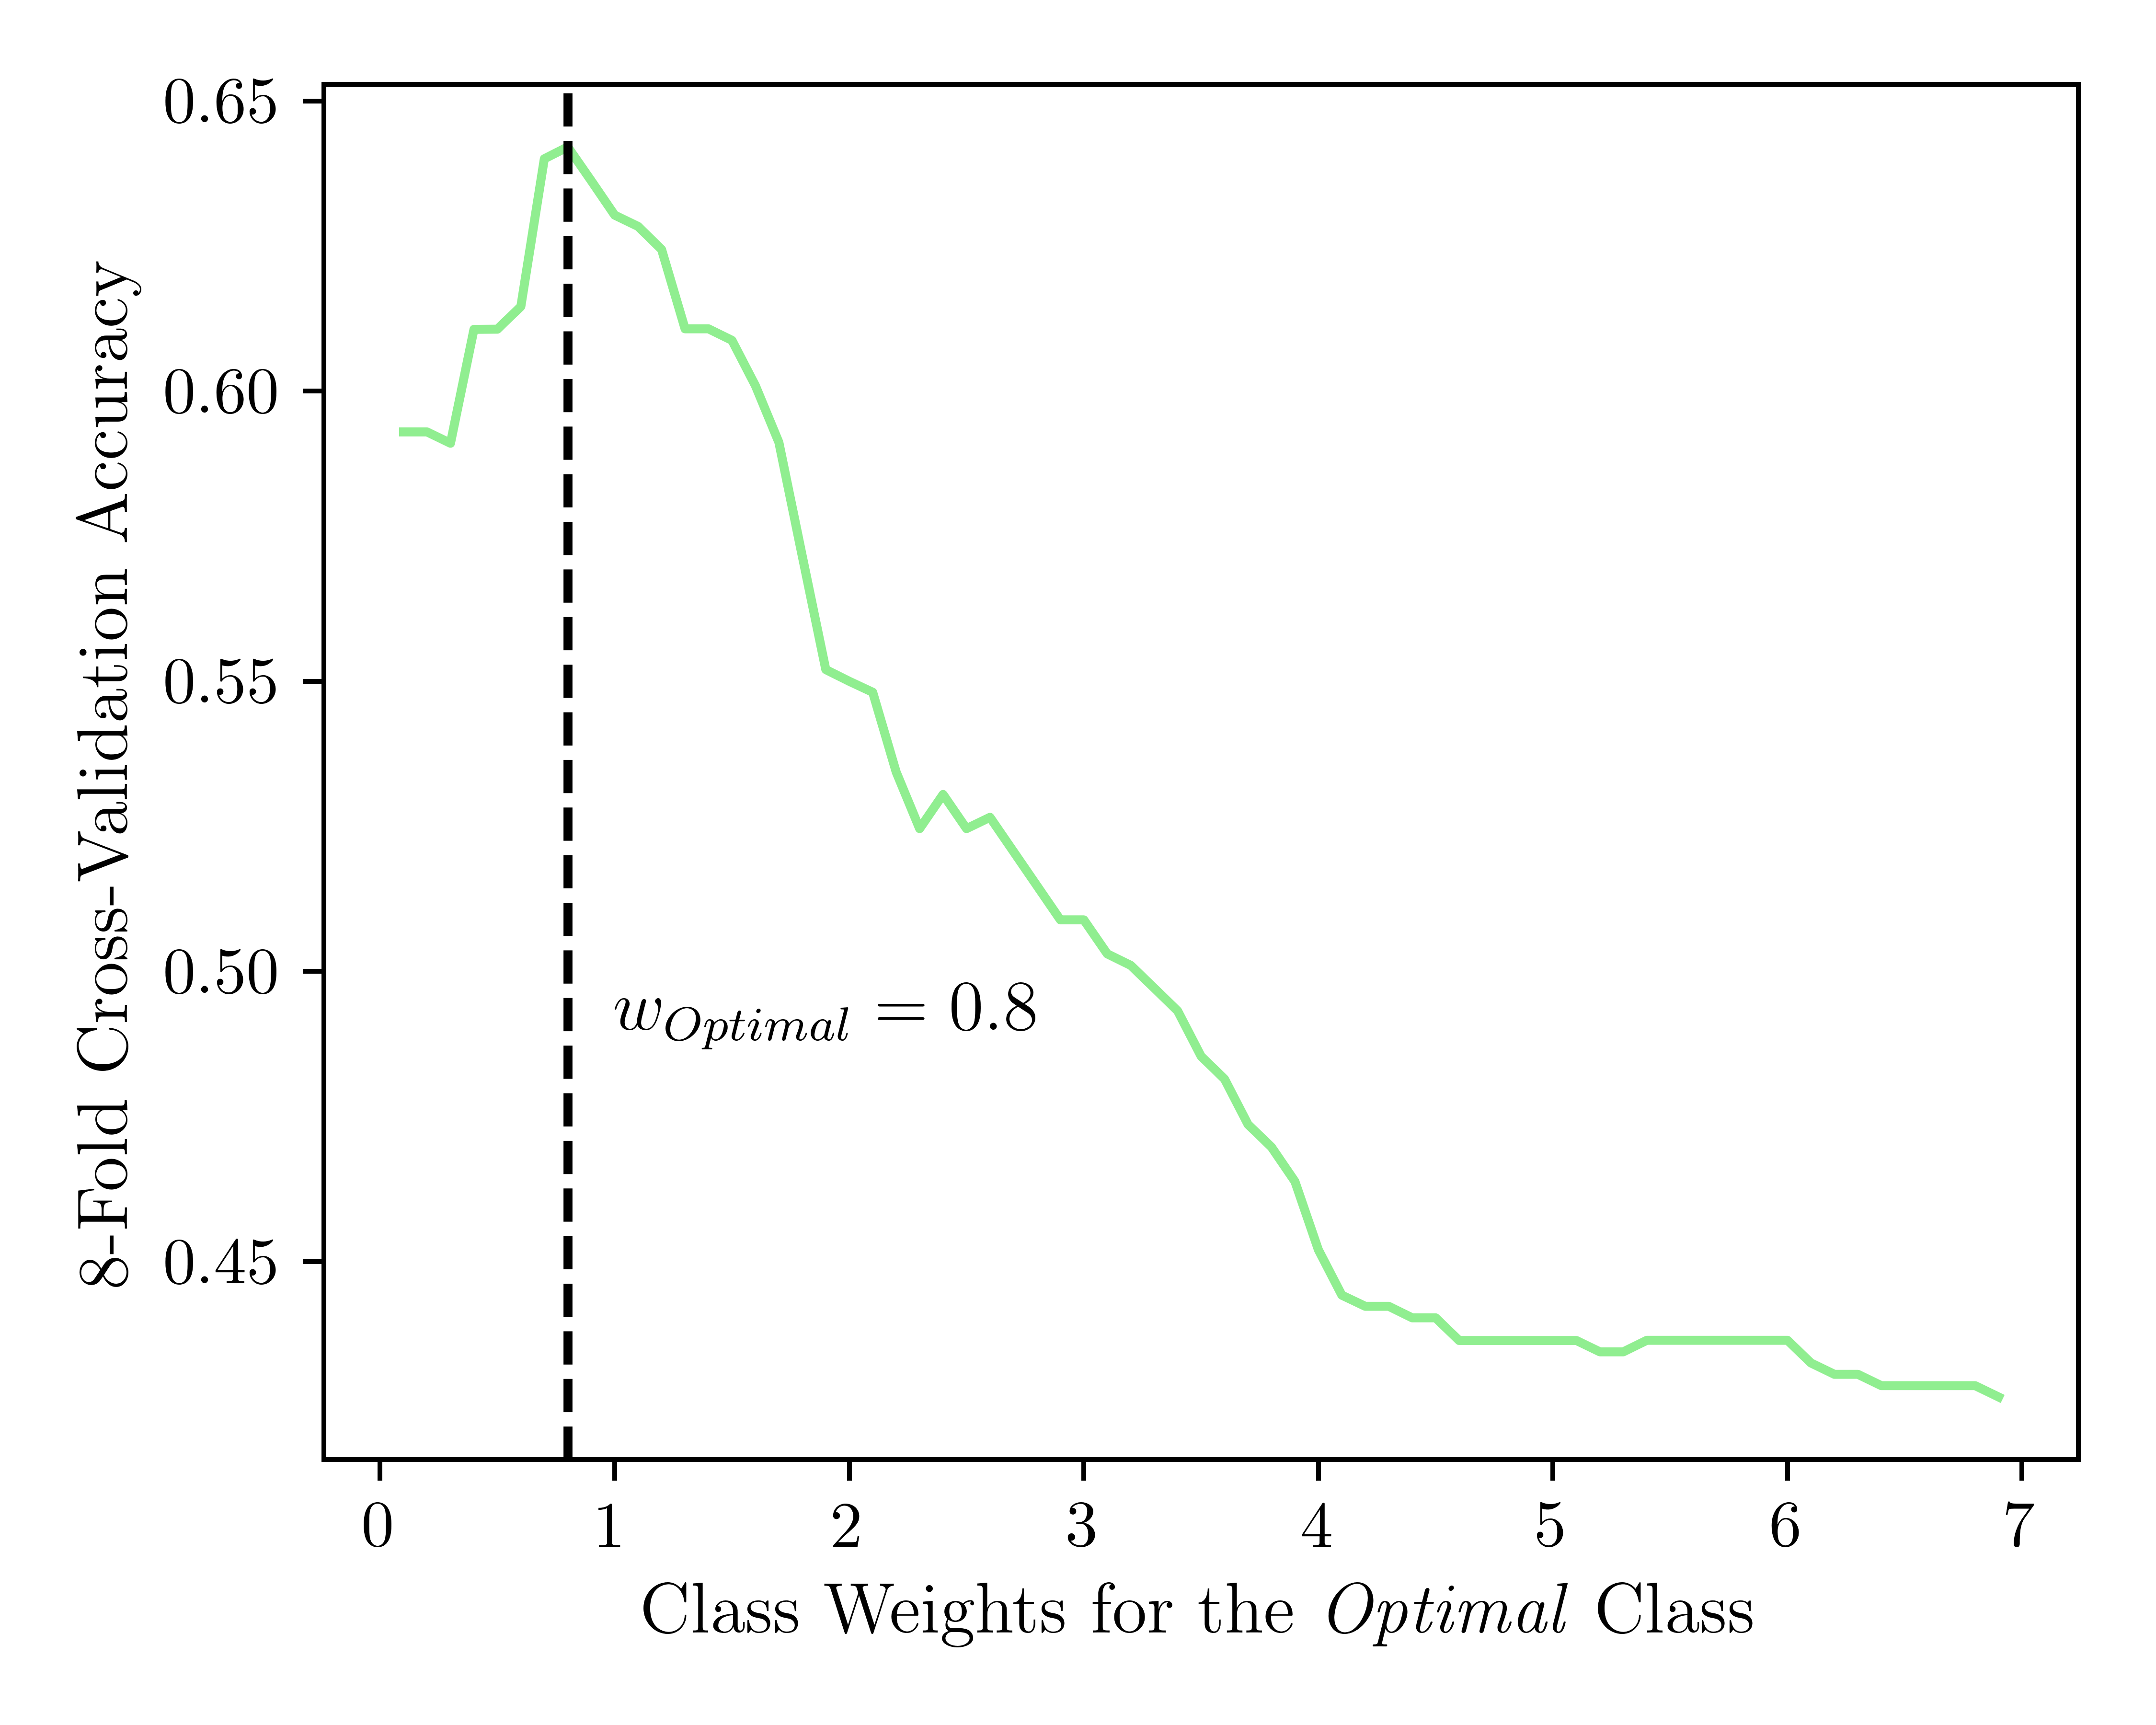
\includegraphics[width=1\linewidth]{assets/SVM_OptimalWeight.png}
    \caption{Effect of the 'Optimal' class weight on SVM model accuracy.}
    \label{svm_weight}
\end{figure}

The weight for the 'Optimal' class that retrieved the highest accuracy was estimated as shown in Figure~\ref{svm_weight} ($w_{Optimal}=0.8$). The remaining classes kept the initially attributed unitary weight. The best parameters found, for this weights, were $C$ 6.93, $\gamma$ auto ($1/n_{features}$), and kernel RBF (Radial Basis Function).

$$\text{RBF kernel: } \exp(-\gamma ||x - x'||^2)$$

\begin{figure}[H]
    \centering
    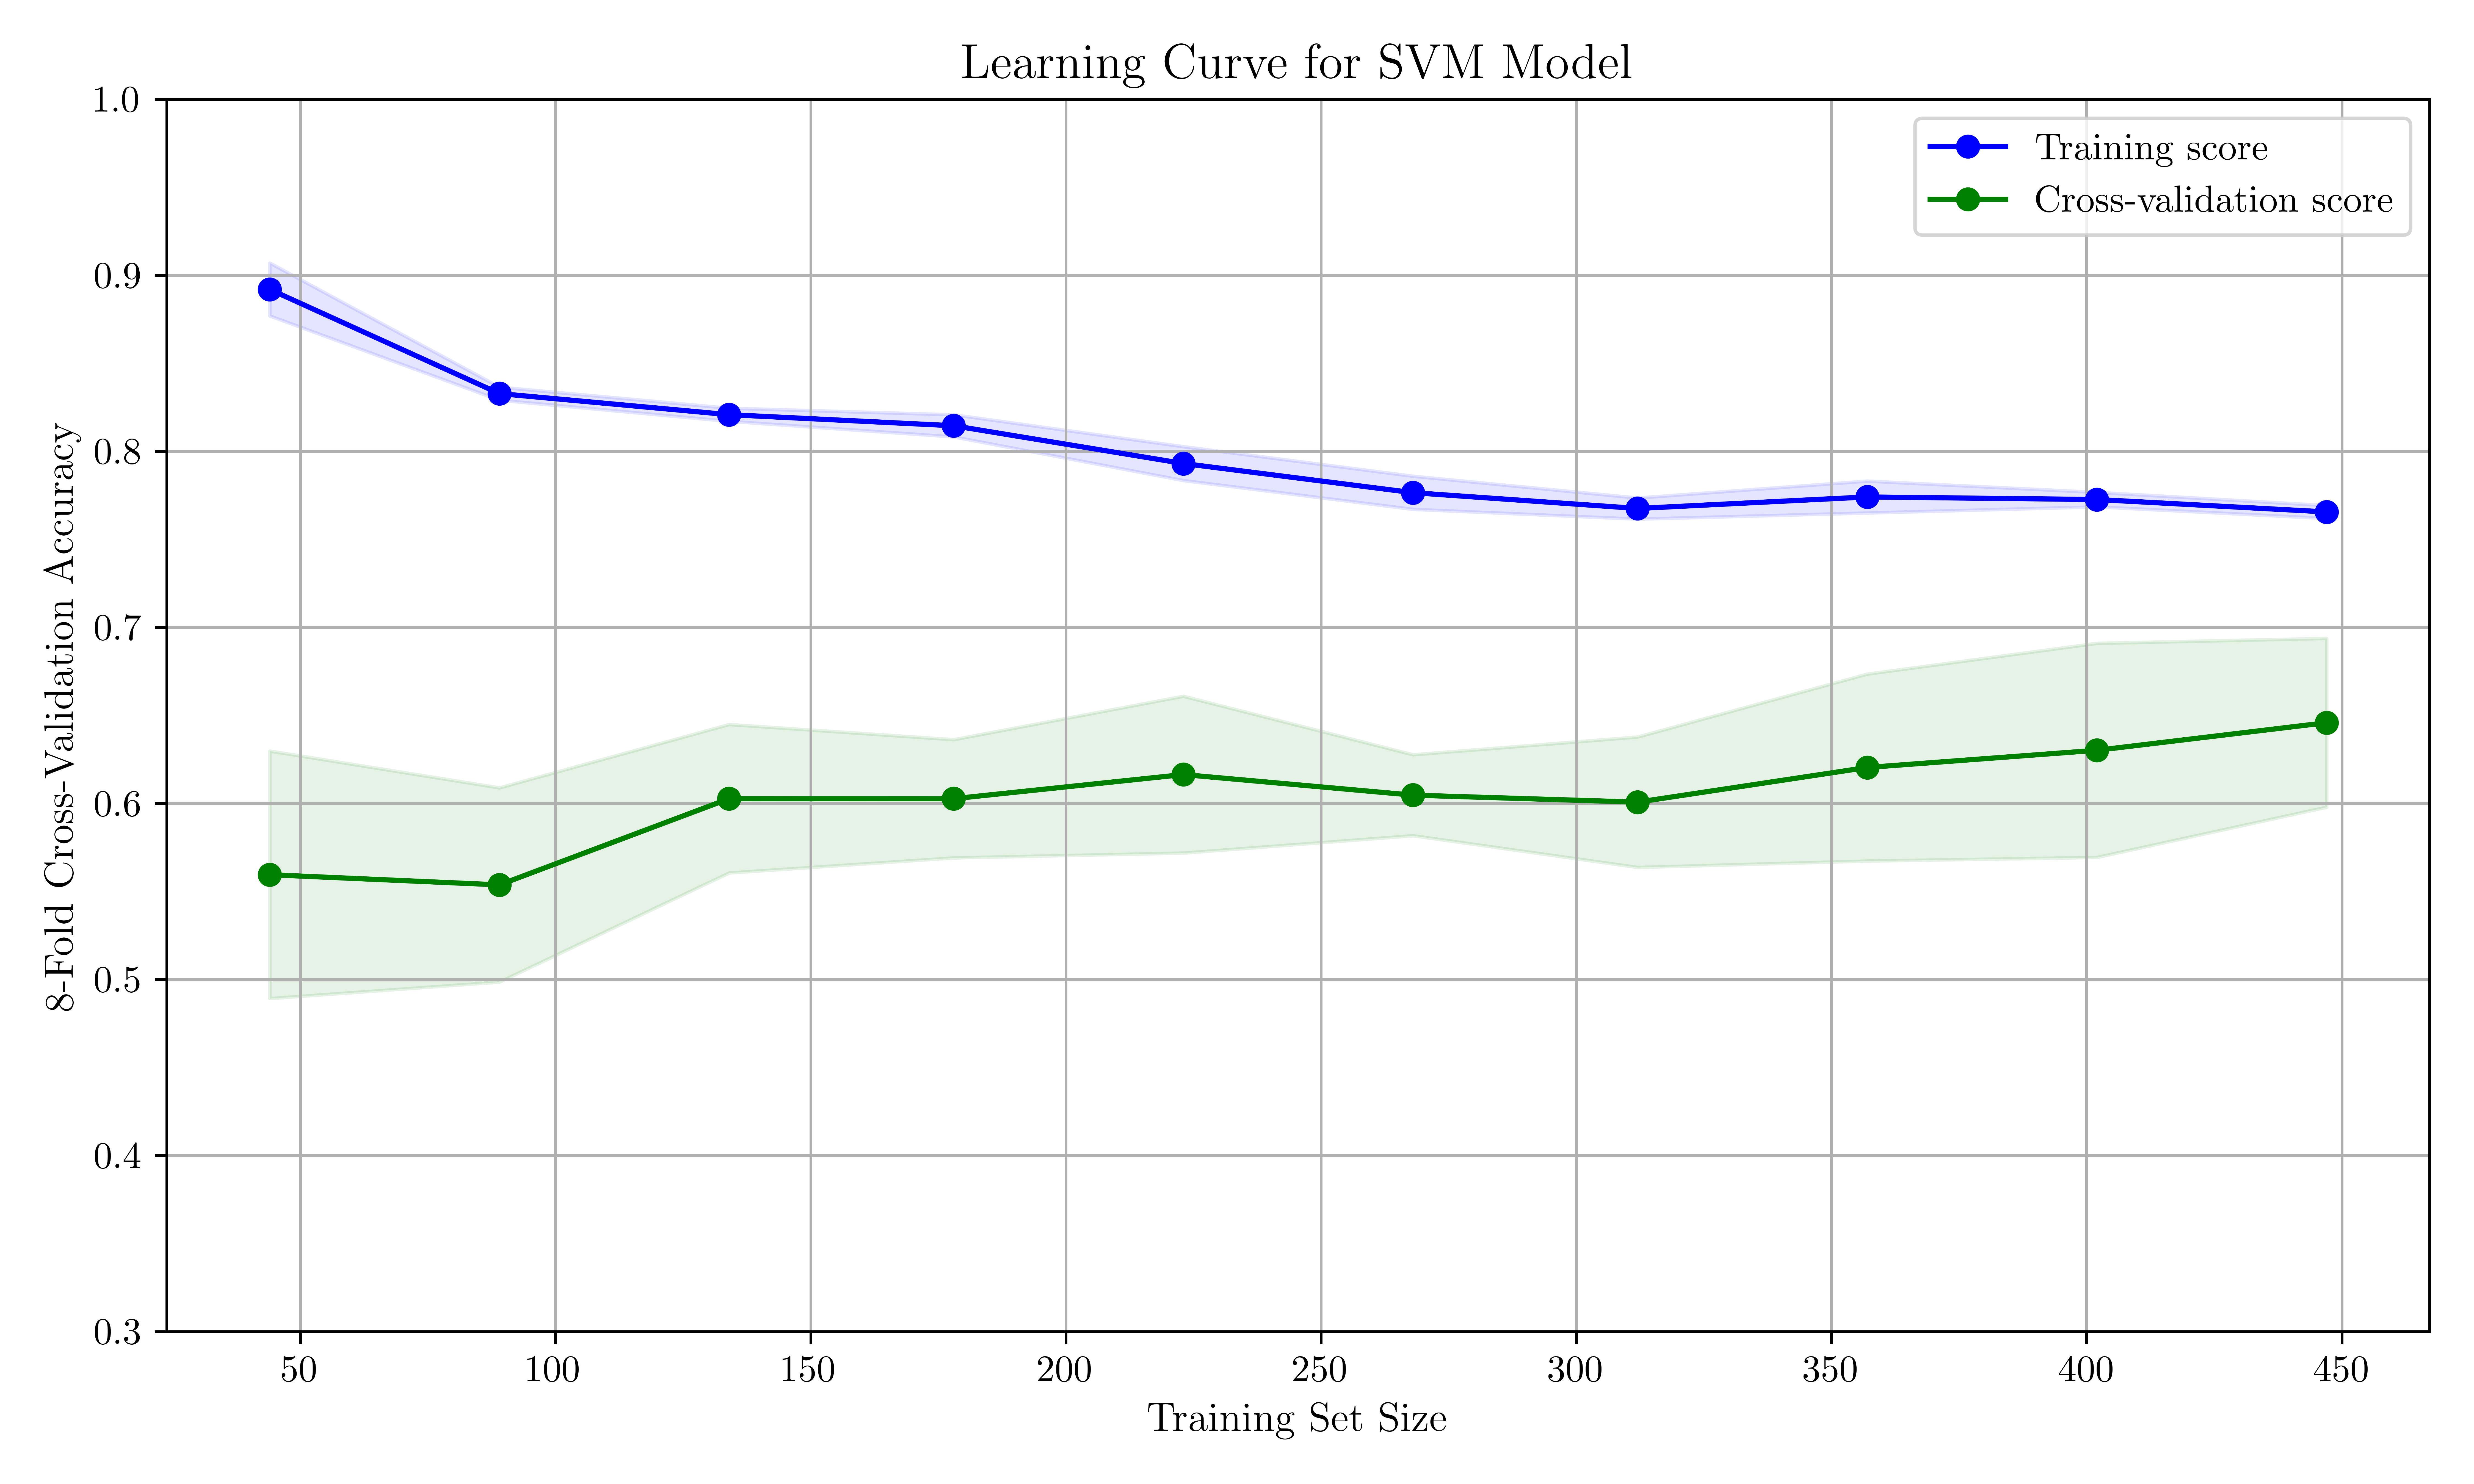
\includegraphics[width=1\linewidth]{assets/SVM_LearningCurve.png}
    \caption{SVM model performance using learning curve representation across varying training data sizes.}
    \label{svm_learningcurve}
\end{figure}

In this case, the learning curves  for both the training and cross-validation sets (Fig. \ref{svm_learningcurve}) converge, with no signs of overfitting. However, it could be beneficial to expand the training dataset further, as the cross-validation score continues to improve. This suggests that the model might still benefit from more data, which could enhance its ability to generalize better.

\begin{figure}[H]
    \centering
    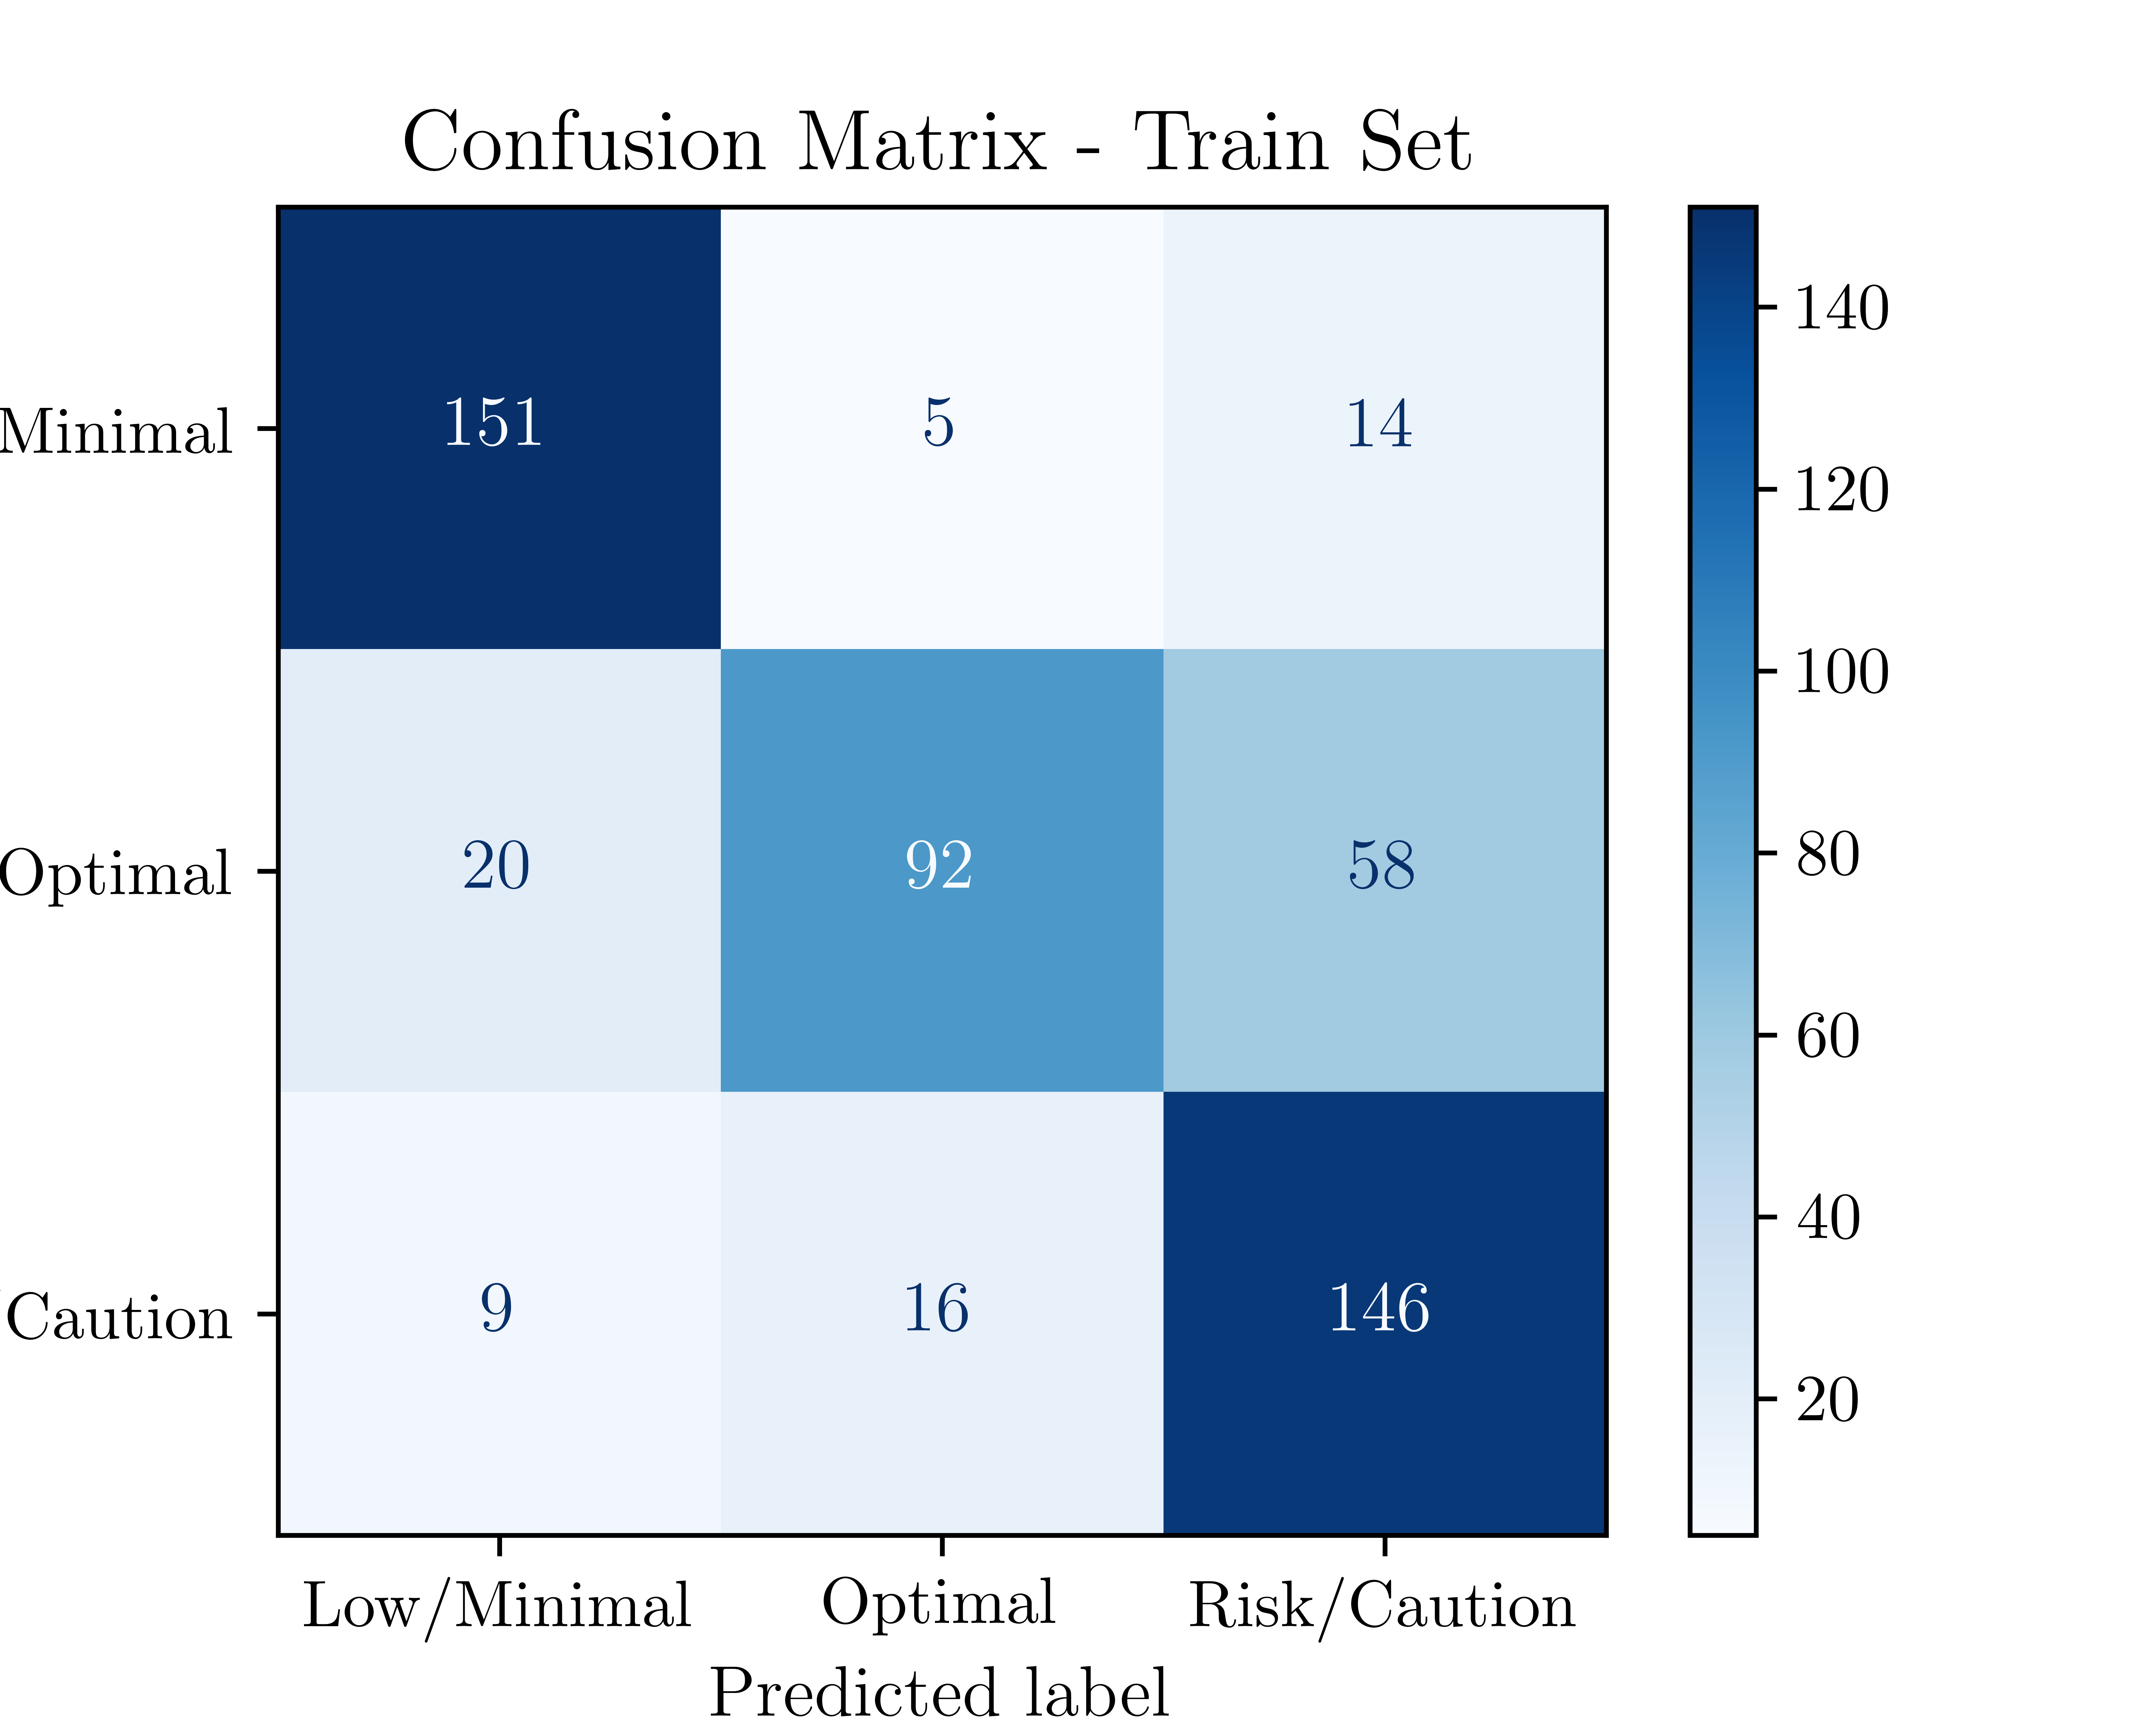
\includegraphics[width=1\linewidth]{assets/SVM_ConfusionMatrixTrain.png}
    \caption{Confusion matrix for the training data of SVM model}
    \label{svm_cm_train}
\end{figure}

\begin{table}[H]
\centering
\caption{Classification report for SVM model performance evaluation on training data.}
\label{crTrainSVM}
\begin{tabular}{lcccccc}
\toprule
\textbf{Class} & \textbf{Precision} & \textbf{Recall} & \textbf{F1-Score} & \textbf{Support} \\
\midrule
Low/Minimal & 0.84 & 0.89 & 0.86 & 170 \\
Optimal & 0.81 & 0.54 & 0.65 & 170 \\
Risk/Caution & 0.67 & 0.85 & 0.75 & 171 \\
\midrule
\textbf{Accuracy} &  &  & 0.76 & 511 \\
\textbf{Macro avg} & 0.77 & 0.76 & 0.75 & 511 \\
\textbf{Weighted avg} & 0.77 & 0.76 & 0.75 & 511 \\
\bottomrule
\end{tabular}
\end{table}

\begin{figure}[H]
    \centering
    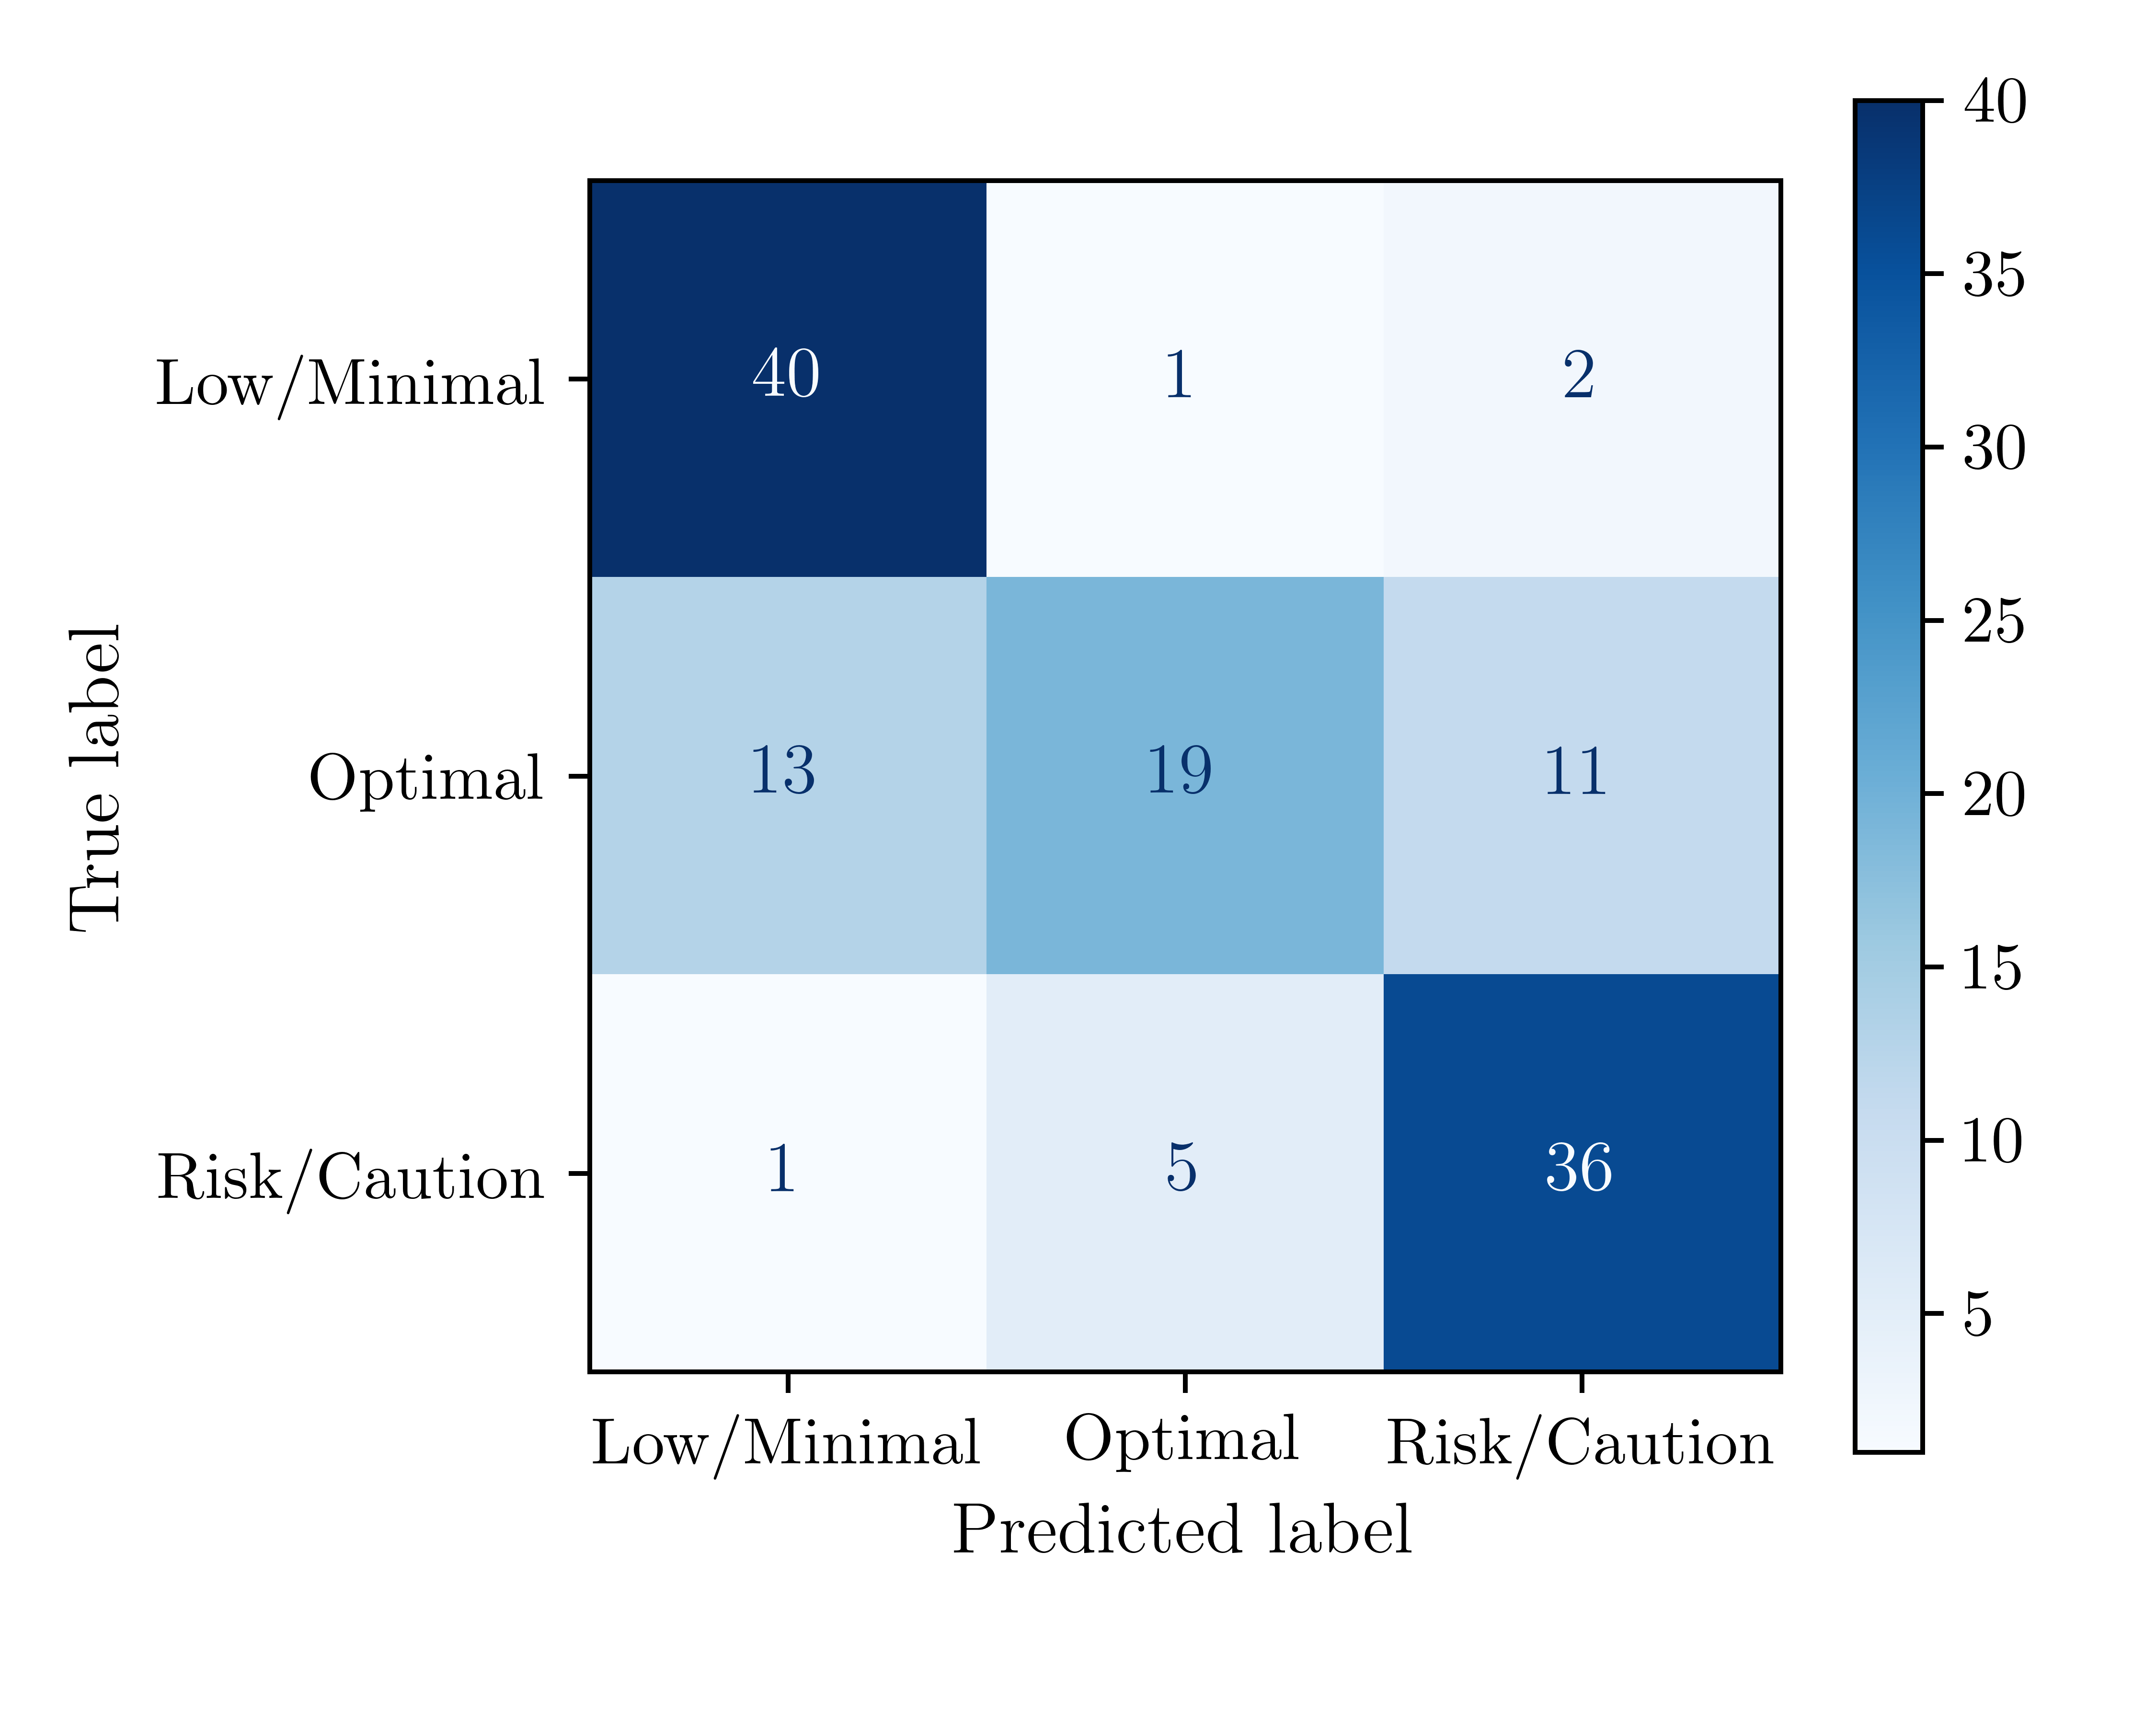
\includegraphics[width=1\linewidth]{assets/SVM_ConfusionMatrixTest.png}
    \caption{Confusion matrix for the test data of SVM model}
    \label{svm_cm_test}
\end{figure}

\begin{table}[H]
\centering
\caption{Classification report for SVM model performance evaluation on test data.}
\label{crTestSVM}
\begin{tabular}{lcccccc}
\toprule
\textbf{Class} & \textbf{Precision} & \textbf{Recall} & \textbf{F1-Score} & \textbf{Support} \\
\midrule
Low/Minimal & 0.74 & 0.93 & 0.82 & 43 \\
Optimal & 0.76 & 0.44 & 0.56 & 43 \\
Risk/Caution & 0.73 & 0.86 & 0.79 & 42 \\
\midrule
\textbf{Accuracy} &  &  & 0.74 & 128 \\
\textbf{Macro avg} & 0.75 & 0.74 & 0.72 & 128 \\
\textbf{Weighted avg} & 0.75 & 0.74 & 0.72 & 128 \\
\bottomrule
\end{tabular}
\end{table}


atendendo as matrizes de cofnusao de treino e de teste (figures \ref{svm_cm_train} and \ref{svm_cm_test}, respectively), verifica-se um bom desempenho na idenfiticacao de todas as classes, principalemente das extremas ('Low/Minimal' and 'Risk/Caution'), tando nos dados de teste como de treino.

quanto aos classification report dos dados de treino e de teste (Tables \ref{crTrainSVM} and \ref{crTestSVM}, respectively), são possiveis verificar resultados consistentes entre ambos os reports. Oberva-se no entando um mua recall para a classe 'Optimal', indicando many missclassification fot this class.


\section{decision tree model}

The decision tree model was developed considering the hyperparameters available and setting ranges for the possible values to be estimated \cite{dtree17}. The ranges were selected taking in consideration the need to minimize the risk of over fitting. The split criteria are among the most commonly used, and the remaining ranges considered for the hyperparameters are presented in Table~\ref{parametrosDTree}.

\begin{table}[H]
\centering
\caption{Decision tree model hyperparameters search space.}
\label{parametrosDTree}
\begin{tabular}{ll}
\toprule
\textbf{Hyperparameter} & \textbf{Possible Values} \\
\midrule
Split Criterion & \{gini, entropy\} \\ 
Max Depth & $[2, 3, \dots, 8]$ \\ 
Min Samples to Split & $[5, 6, \dots, 20]$ \\ 
Min Samples per Leaf & $[3, 4, \dots, 10]$ \\
\bottomrule
\end{tabular}
\end{table}

The max tree depth selected was 4, minimium samples to split 11, minimium samples per leaf 7, and the split criterion entropy ($H$)

$$H(\text{node}) = - \sum_{\text{Class }_j} p(\text{Class}_j | \text{node}) \log p(\text{Class}_j | \text{node})$$

%%%%%%%%%%
% https://scikit-learn.org/dev/modules/generated/sklearn.tree.DecisionTreeClassifier.html

%max depth: (The deeper the tree, the more splits it has and it captures more information about the data)

%min sample split: (When we increase this parameter, the tree becomes more constrained as it has to consider more samples at each node.)

%min samples leaf: (This parameter is similar to min samples splits, however, this describe the minimum number of samples of samples at the leafs, the base of the tree.)

%splitter: best (to choose the best split at each node instead of 'random')

%criterion: (The function to measure the quality of a split. Shannon information gain)
%%%%%%%%%%

The optimized DTree resulted in the structure as seen in Figure~\ref{dtree_tree}.

\begin{figure}[H]
    \centering
    \includegraphics[width=1\linewidth]{assets/DTREE_Tree.png}
    \caption{Visualization of the decision tree model after optimization using randomized search.}
    \label{dtree_tree}
\end{figure}

The decision paths are characterized by the certainty in each node, highlighted by the color saturation for each of the classes ('Low/Minimal', 'Optimal', 'Risk/Caution'). The diminished proportion of end nodes with higher color saturation for 'Optimal' when comparing with the other classes is noteworthy, and consistent with the observations for the remaining models.

\begin{figure}[H]
    \centering
    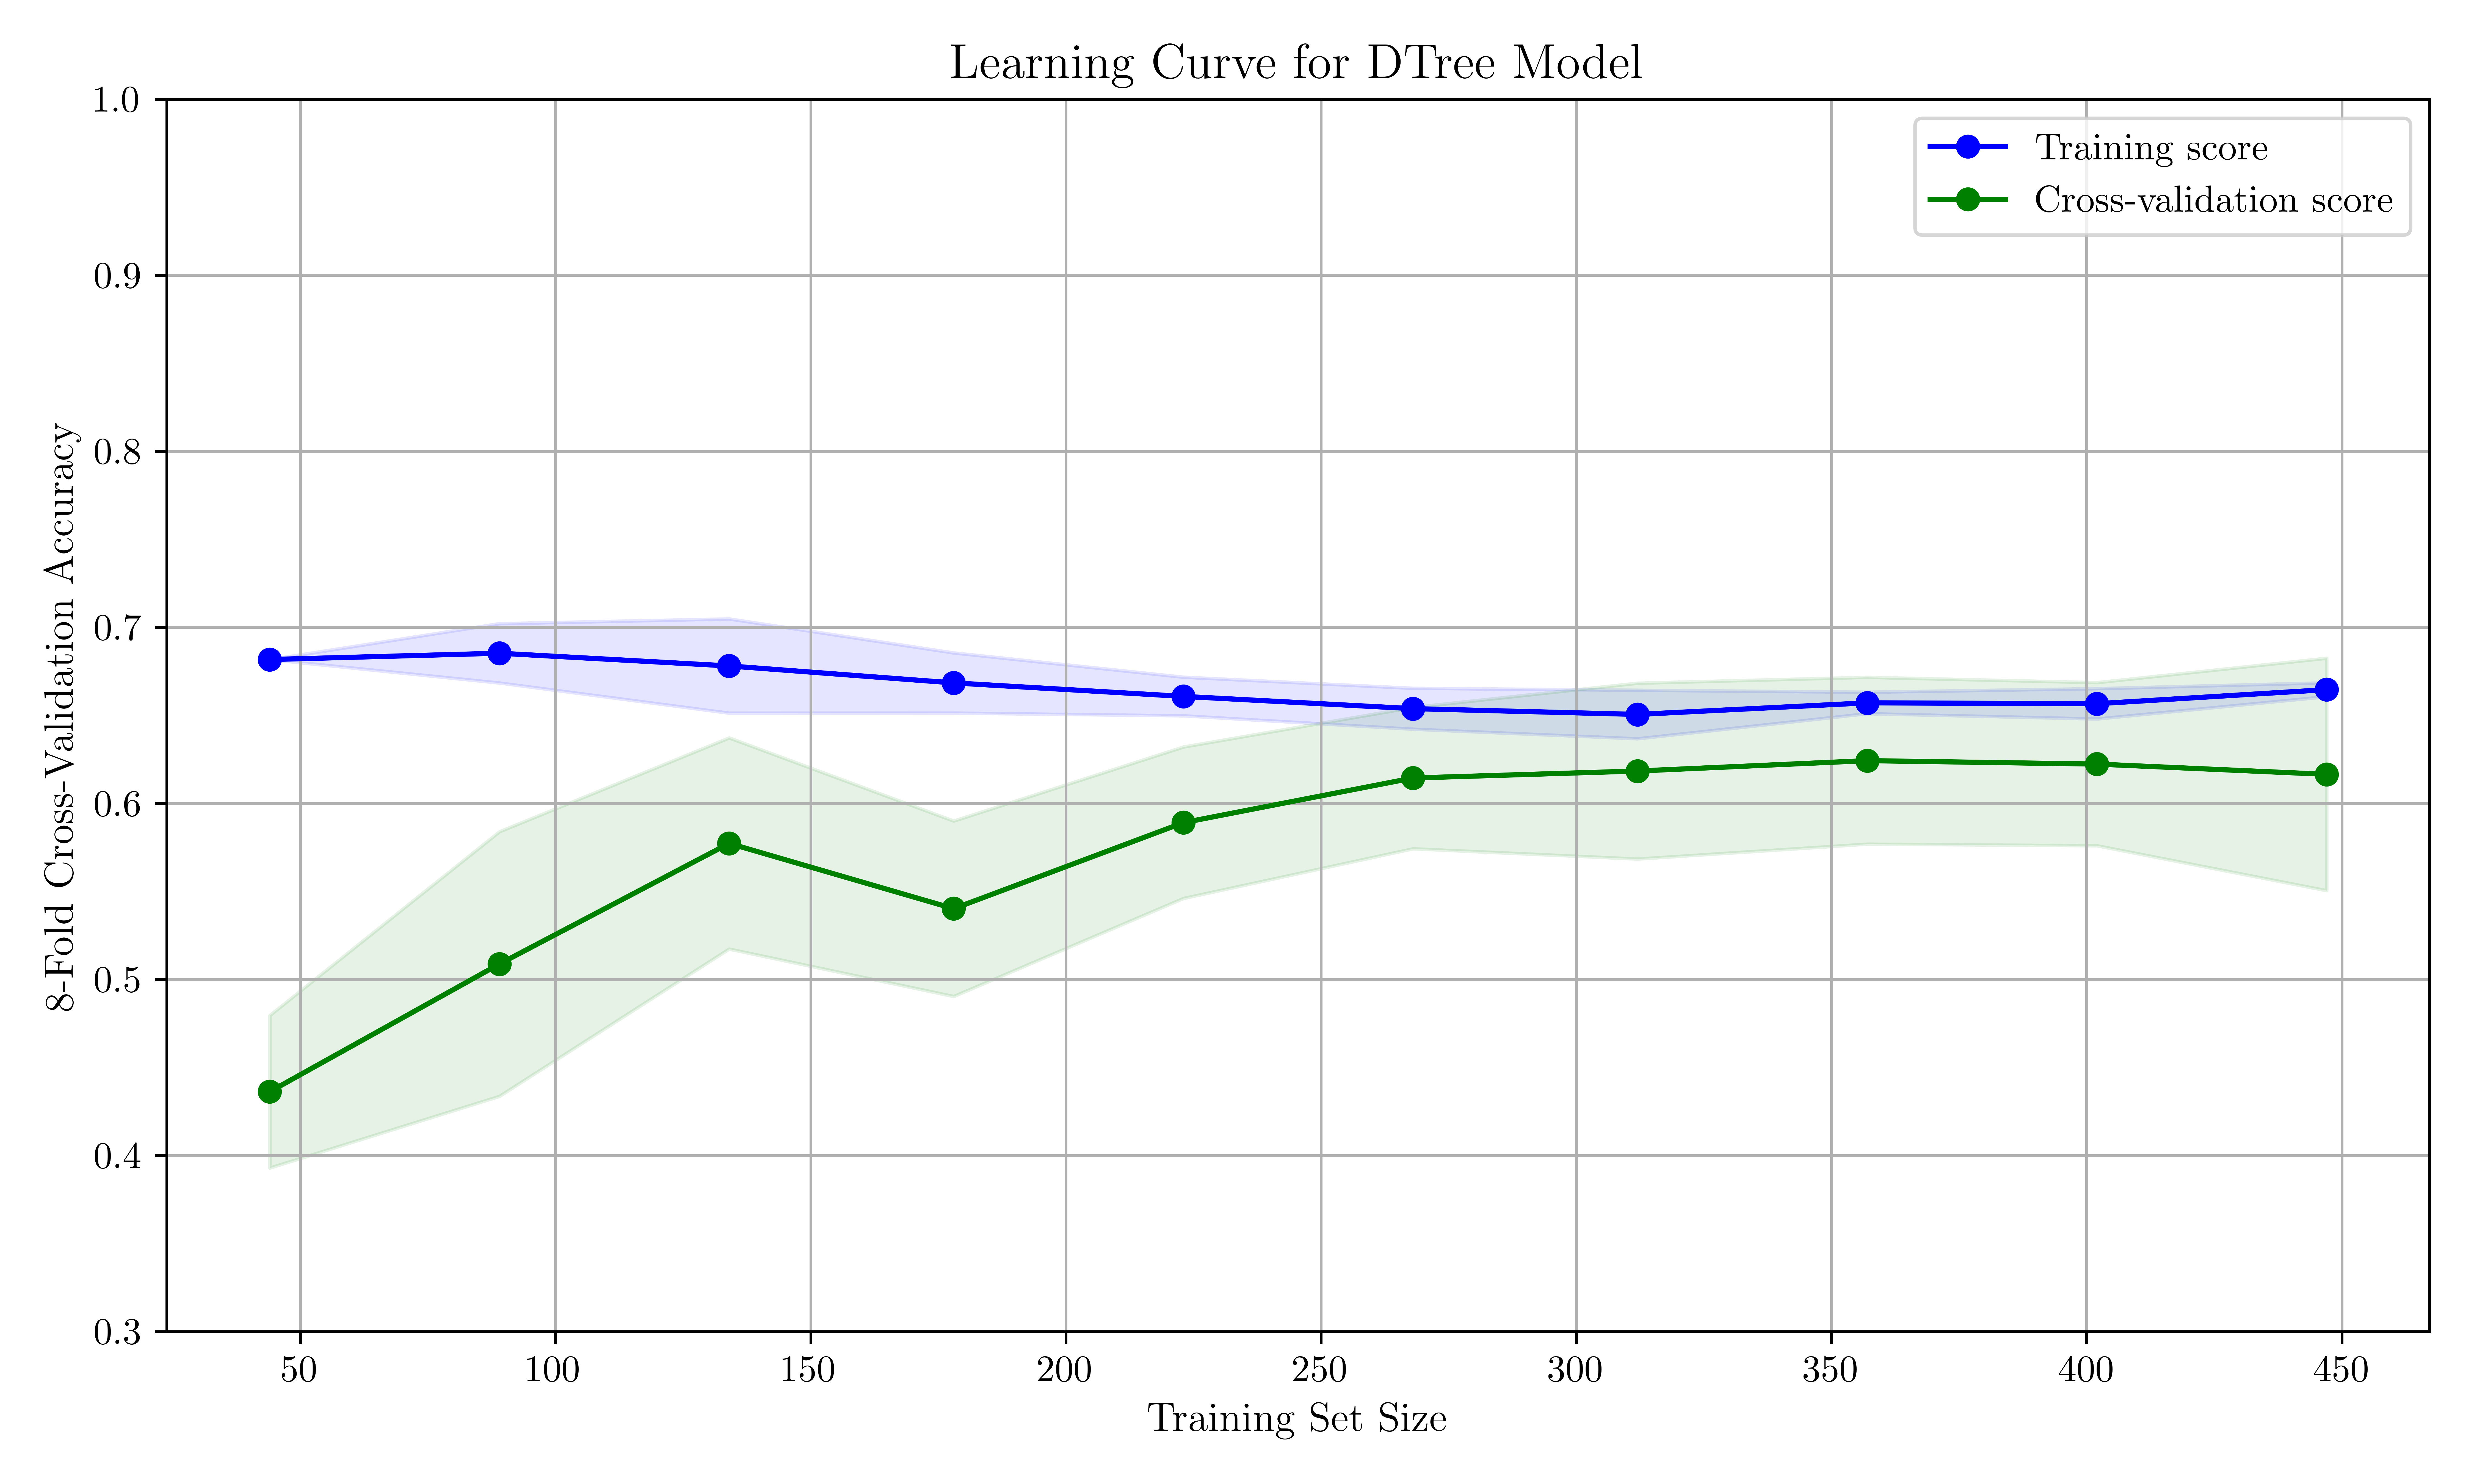
\includegraphics[width=1\linewidth]{assets/DTREE_LearningCurve.png}
    \caption{Analysis of decision tree model performance using learning curve representation across varying training data sizes.}
    \label{dtree_lcurve}
\end{figure}

Ao analisar as learning curves {Fig. \ref{dtree_lcurve}}, for both the training and cross-validation sets, é possivel verificar que até ao training size de 250, o modelo beneficia significatvemente do aumento dos dados, sendo que após este training size, he cross-validation score stabilized paralelamente ao training socre, revelando convergencia, sem sinais de overfitting.

%sera q cale a pena dizer q no fim ela começa a descer pelo q poderia ser ovefitting ?

\begin{figure}[H]
    \centering
    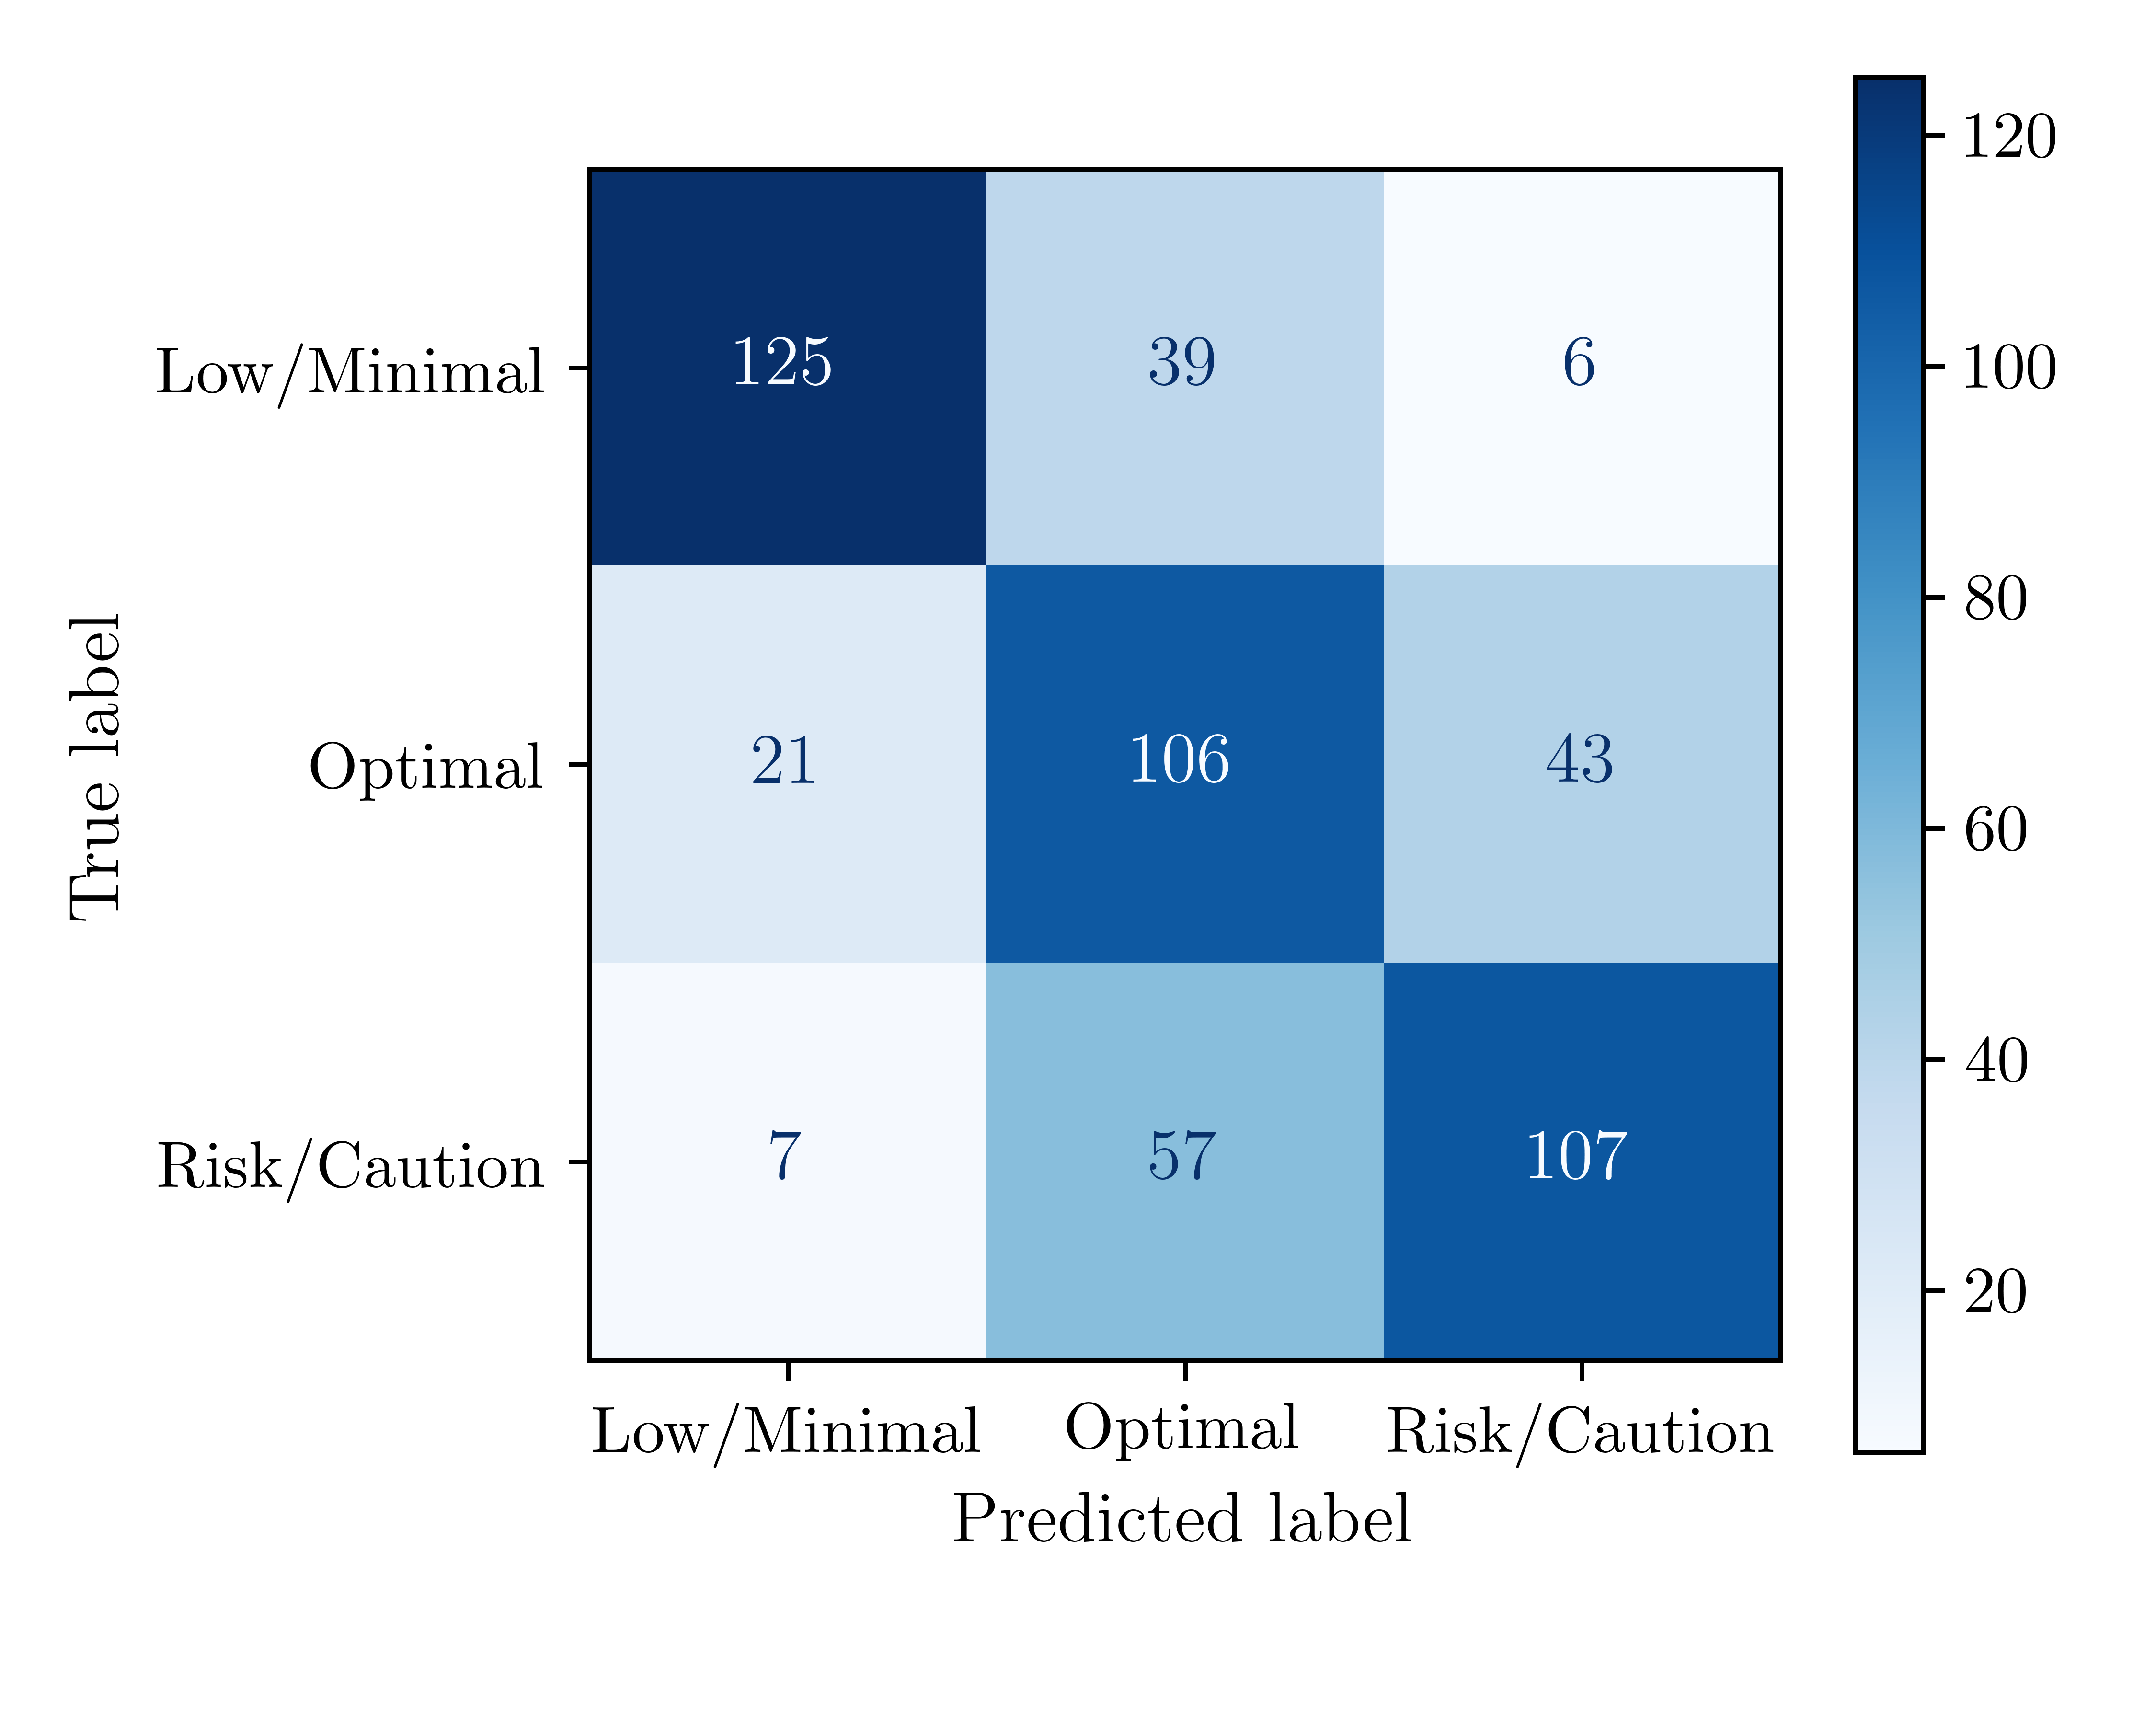
\includegraphics[width=1\linewidth]{assets/DTREE_ConfusionMatrixTrain.png}
    \caption{Evaluation of decision tree model performance on training data performance via confusion matrix.}
    \label{dtree_cmtrain}
\end{figure}

\begin{table}[H]
\centering
\caption{Classification report for decision tree model performance evaluation on training data.}
\label{cr_dtree_train}
\begin{tabular}{lcccccc}
\toprule
\textbf{Class} & \textbf{Precision} & \textbf{Recall} & \textbf{F1-Score} & \textbf{Support} \\
\midrule
Low/Minimal & 0.82 & 0.74 & 0.77 & 170 \\
Optimal & 0.52 & 0.62 & 0.57 & 170 \\
Risk/Caution & 0.69 & 0.63 & 0.65 & 171 \\
\midrule
\textbf{Accuracy} &  &  & 0.66 & 511 \\
\textbf{Macro avg} & 0.68 & 0.66 & 0.67 & 511 \\
\textbf{Weighted avg} & 0.68 & 0.66 & 0.67 & 511 \\
\bottomrule
\end{tabular}
\end{table}

\subsection{resultados de teste}

\begin{figure}[H]
    \centering
    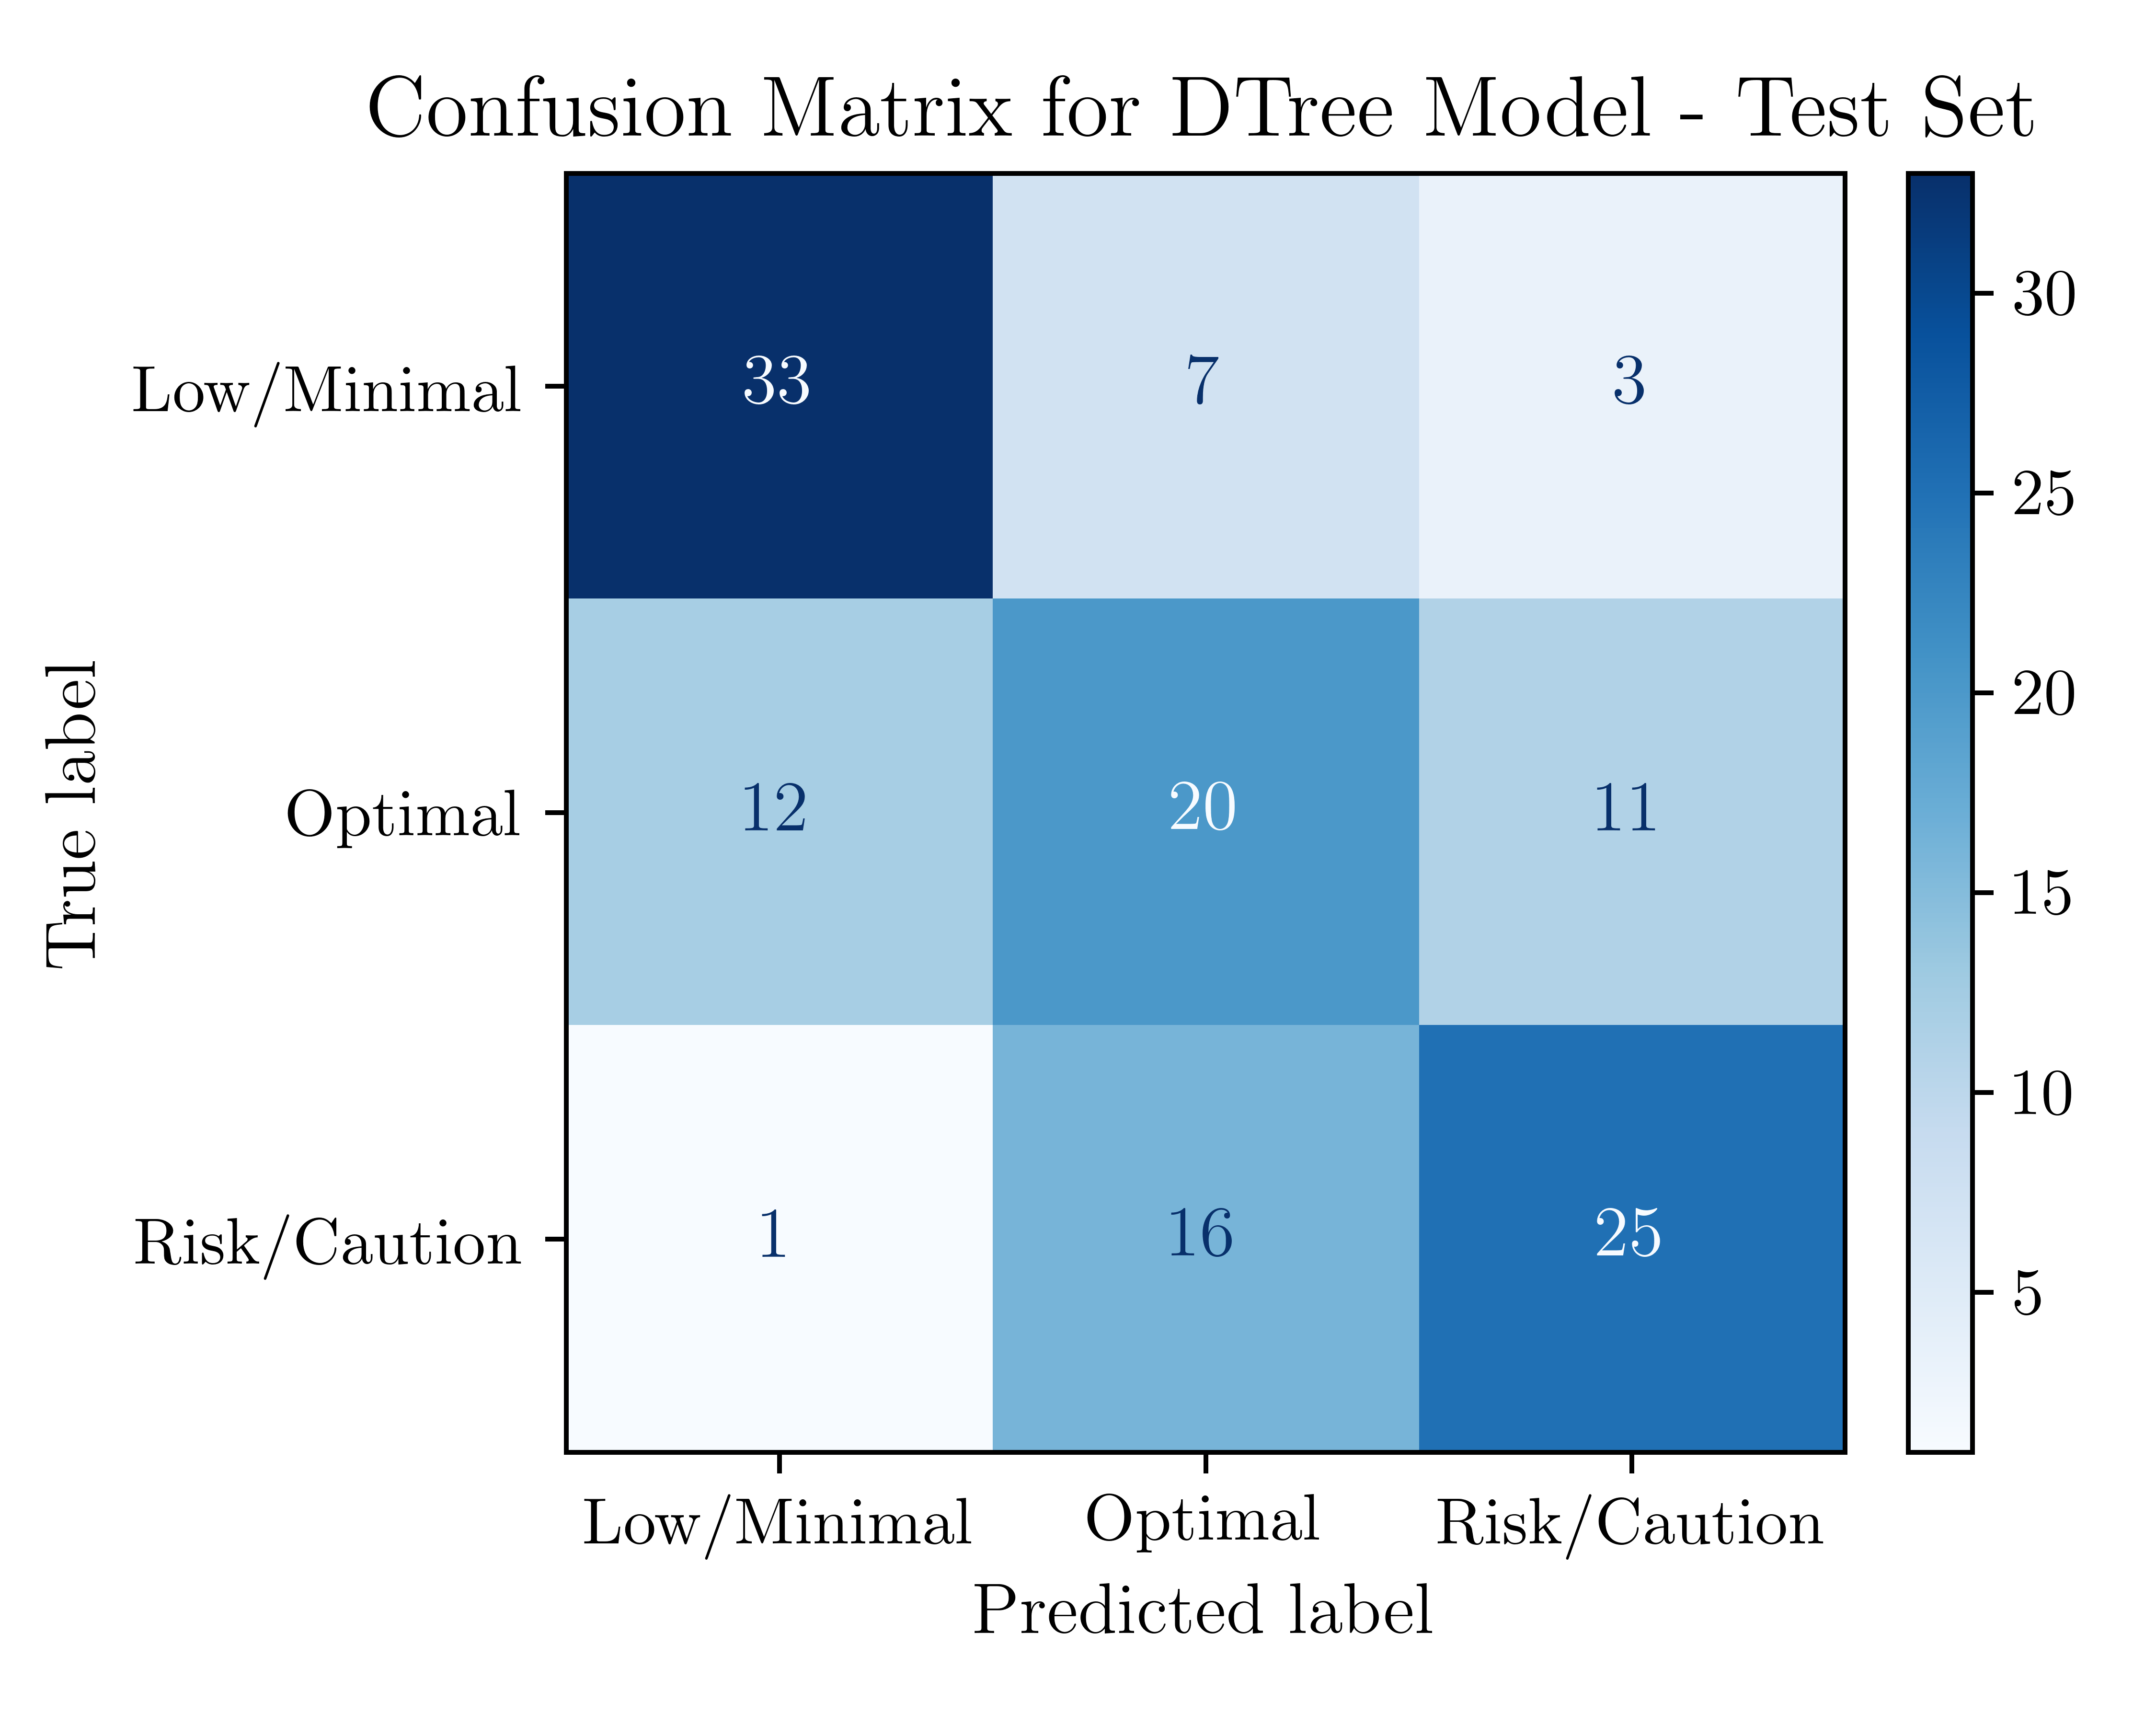
\includegraphics[width=1\linewidth]{assets/DTREE_ConfusionMatrixTest.png}
    \caption{Evaluation of decision tree model performance on test data performance via confusion matrix.}
    \label{dtree_cmtest}
\end{figure}

\begin{table}[H]
\centering
\caption{Classification report for decision tree model performance evaluation on test data.}
\label{cr_dtree_test}
\begin{tabular}{lcccccc}
\toprule
\textbf{Class} & \textbf{Precision} & \textbf{Recall} & \textbf{F1-Score} & \textbf{Support} \\
\midrule
Low/Minimal & 0.72 & 0.77 & 0.74 & 43 \\
Optimal & 0.47 & 0.47 & 0.47 & 43 \\
Risk/Caution & 0.64 & 0.60 & 0.62 & 43 \\
\midrule
\textbf{Accuracy} &  &  & 0.61 & 128 \\
\textbf{Macro avg} & 0.61 & 0.61 & 0.61 & 128 \\
\textbf{Weighted avg} & 0.61 & 0.61 & 0.61 & 128 \\
\bottomrule
\end{tabular}
\end{table}

Tendo em conta as matrizes de confusao relativamente aos daods de treino e de teste (figures \ref{dtree_cmtrain} and \ref{dtree_cmtest}, respectively), é possivel verificar uma pequena confusão do modelo na classificacao das classes 'Optimal' and 'Risk/Caution', mas uma classficiacao bastante satisfcatoria na classificacao da classe 'Low/Optimal'.

Quanto ao metricas de avalicao do modelo apresetnadas nos classificaions reports, presenteded in the tables \ref{cr_dtree_train} and \ref{cr_dtree_test}, nota-se que de facto as métricas relativas à classe 'Low/Minimal' correspondem às expetativas criadas pelas matrizes de confução. Para além disso, a nível global, tanto os resultados de teste como os de treino são semelhantes, não levantando suspeitras sobre overffintg, o que é satisfatório.



\section{analise de resultados e comp de modelos}

\subsection{metricas ou resultados idk}

Para comparar o desempenho dos diferentes modelos e selecionar aquele com maior capacidade de classificação dentro do contexto, foram gerados box plots para analisar várias métricas de desempenho. O processo de validação cruzada foi realizado utilizando 8 folds no conjunto de dados. Em cada iteração, os modelos foram treinados com 7 folds e testados no fold restante. As métricas de desempenho (precision, recall, f1-score e accuracy) foram calculadas para cada iteração e, posteriormente, usadas para avaliar o desempenho global de cada modelo. Para cada modelo, foram aplicados os hiperparâmetros ótimos definidos anteriormente.

\begin{figure}[H]
    \centering
    \begin{subfigure}[1]{\linewidth}
        \centering
        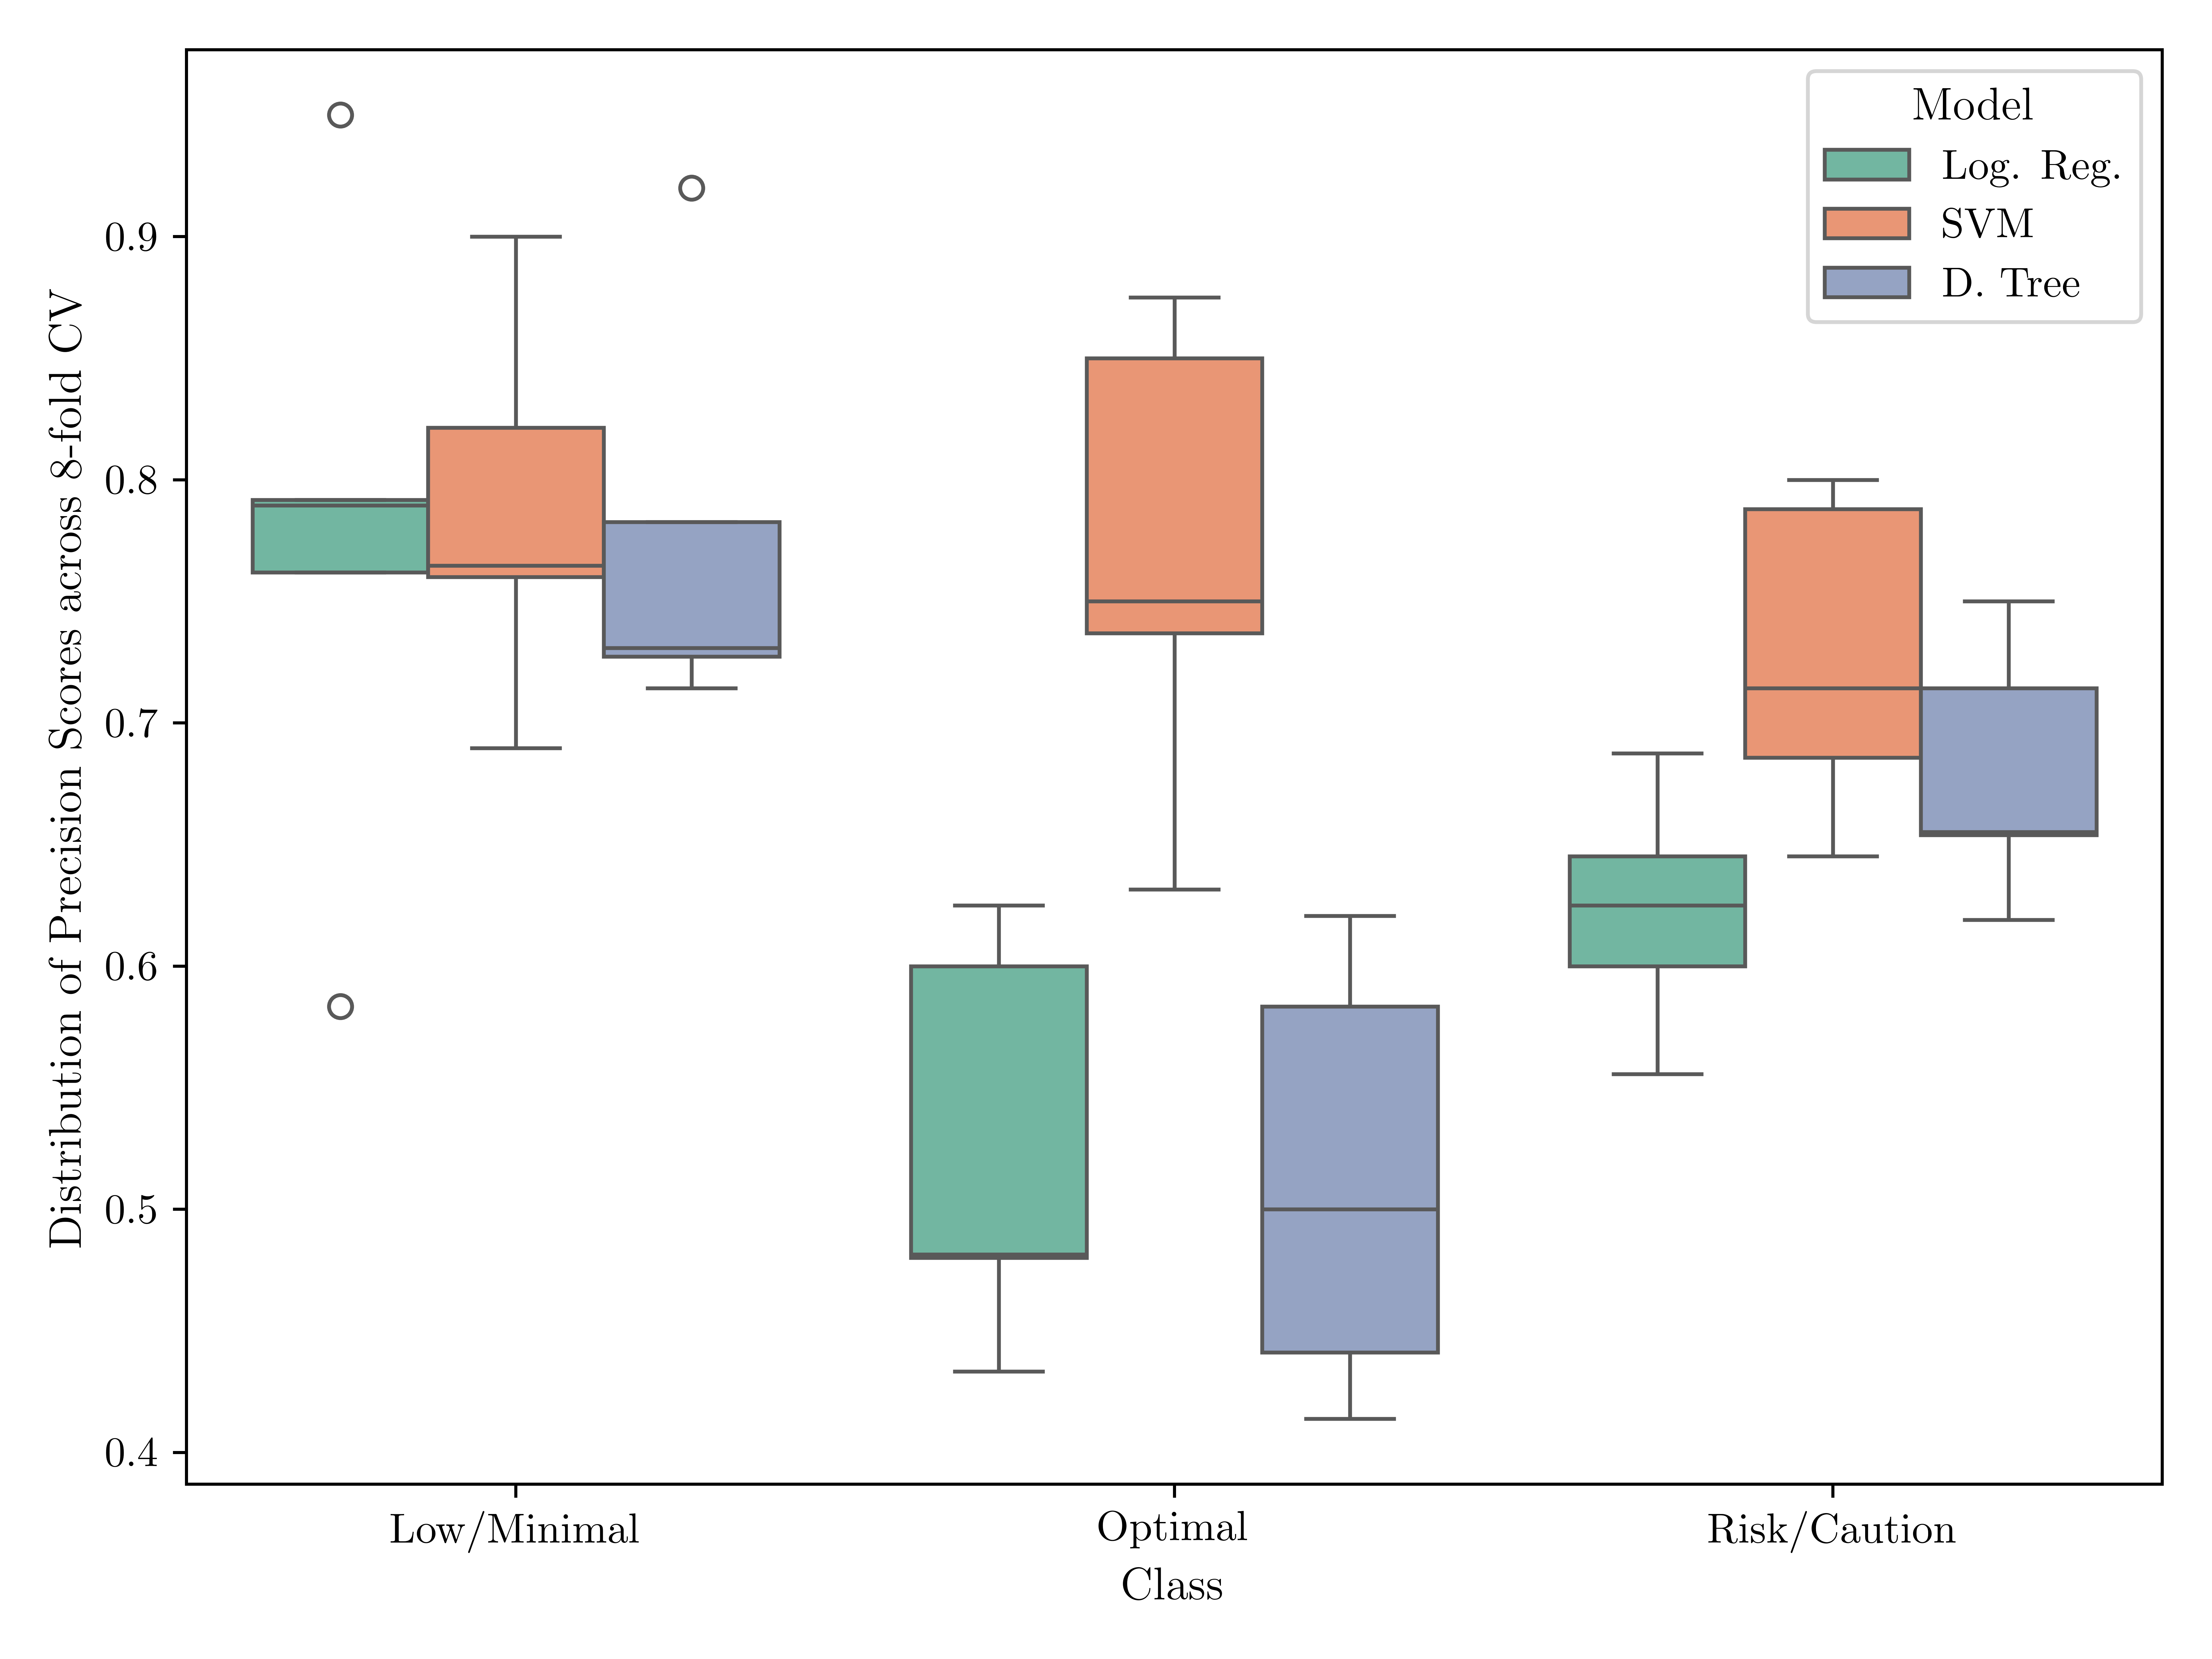
\includegraphics[width=1\linewidth]{assets/box_precision.png}
        \caption{Precision scores across 8-fold cross-validation.}
        \label{box_precision}
    \end{subfigure}
    
    \vspace{0.5cm}

    \begin{subfigure}[1]{\linewidth}
        \centering
        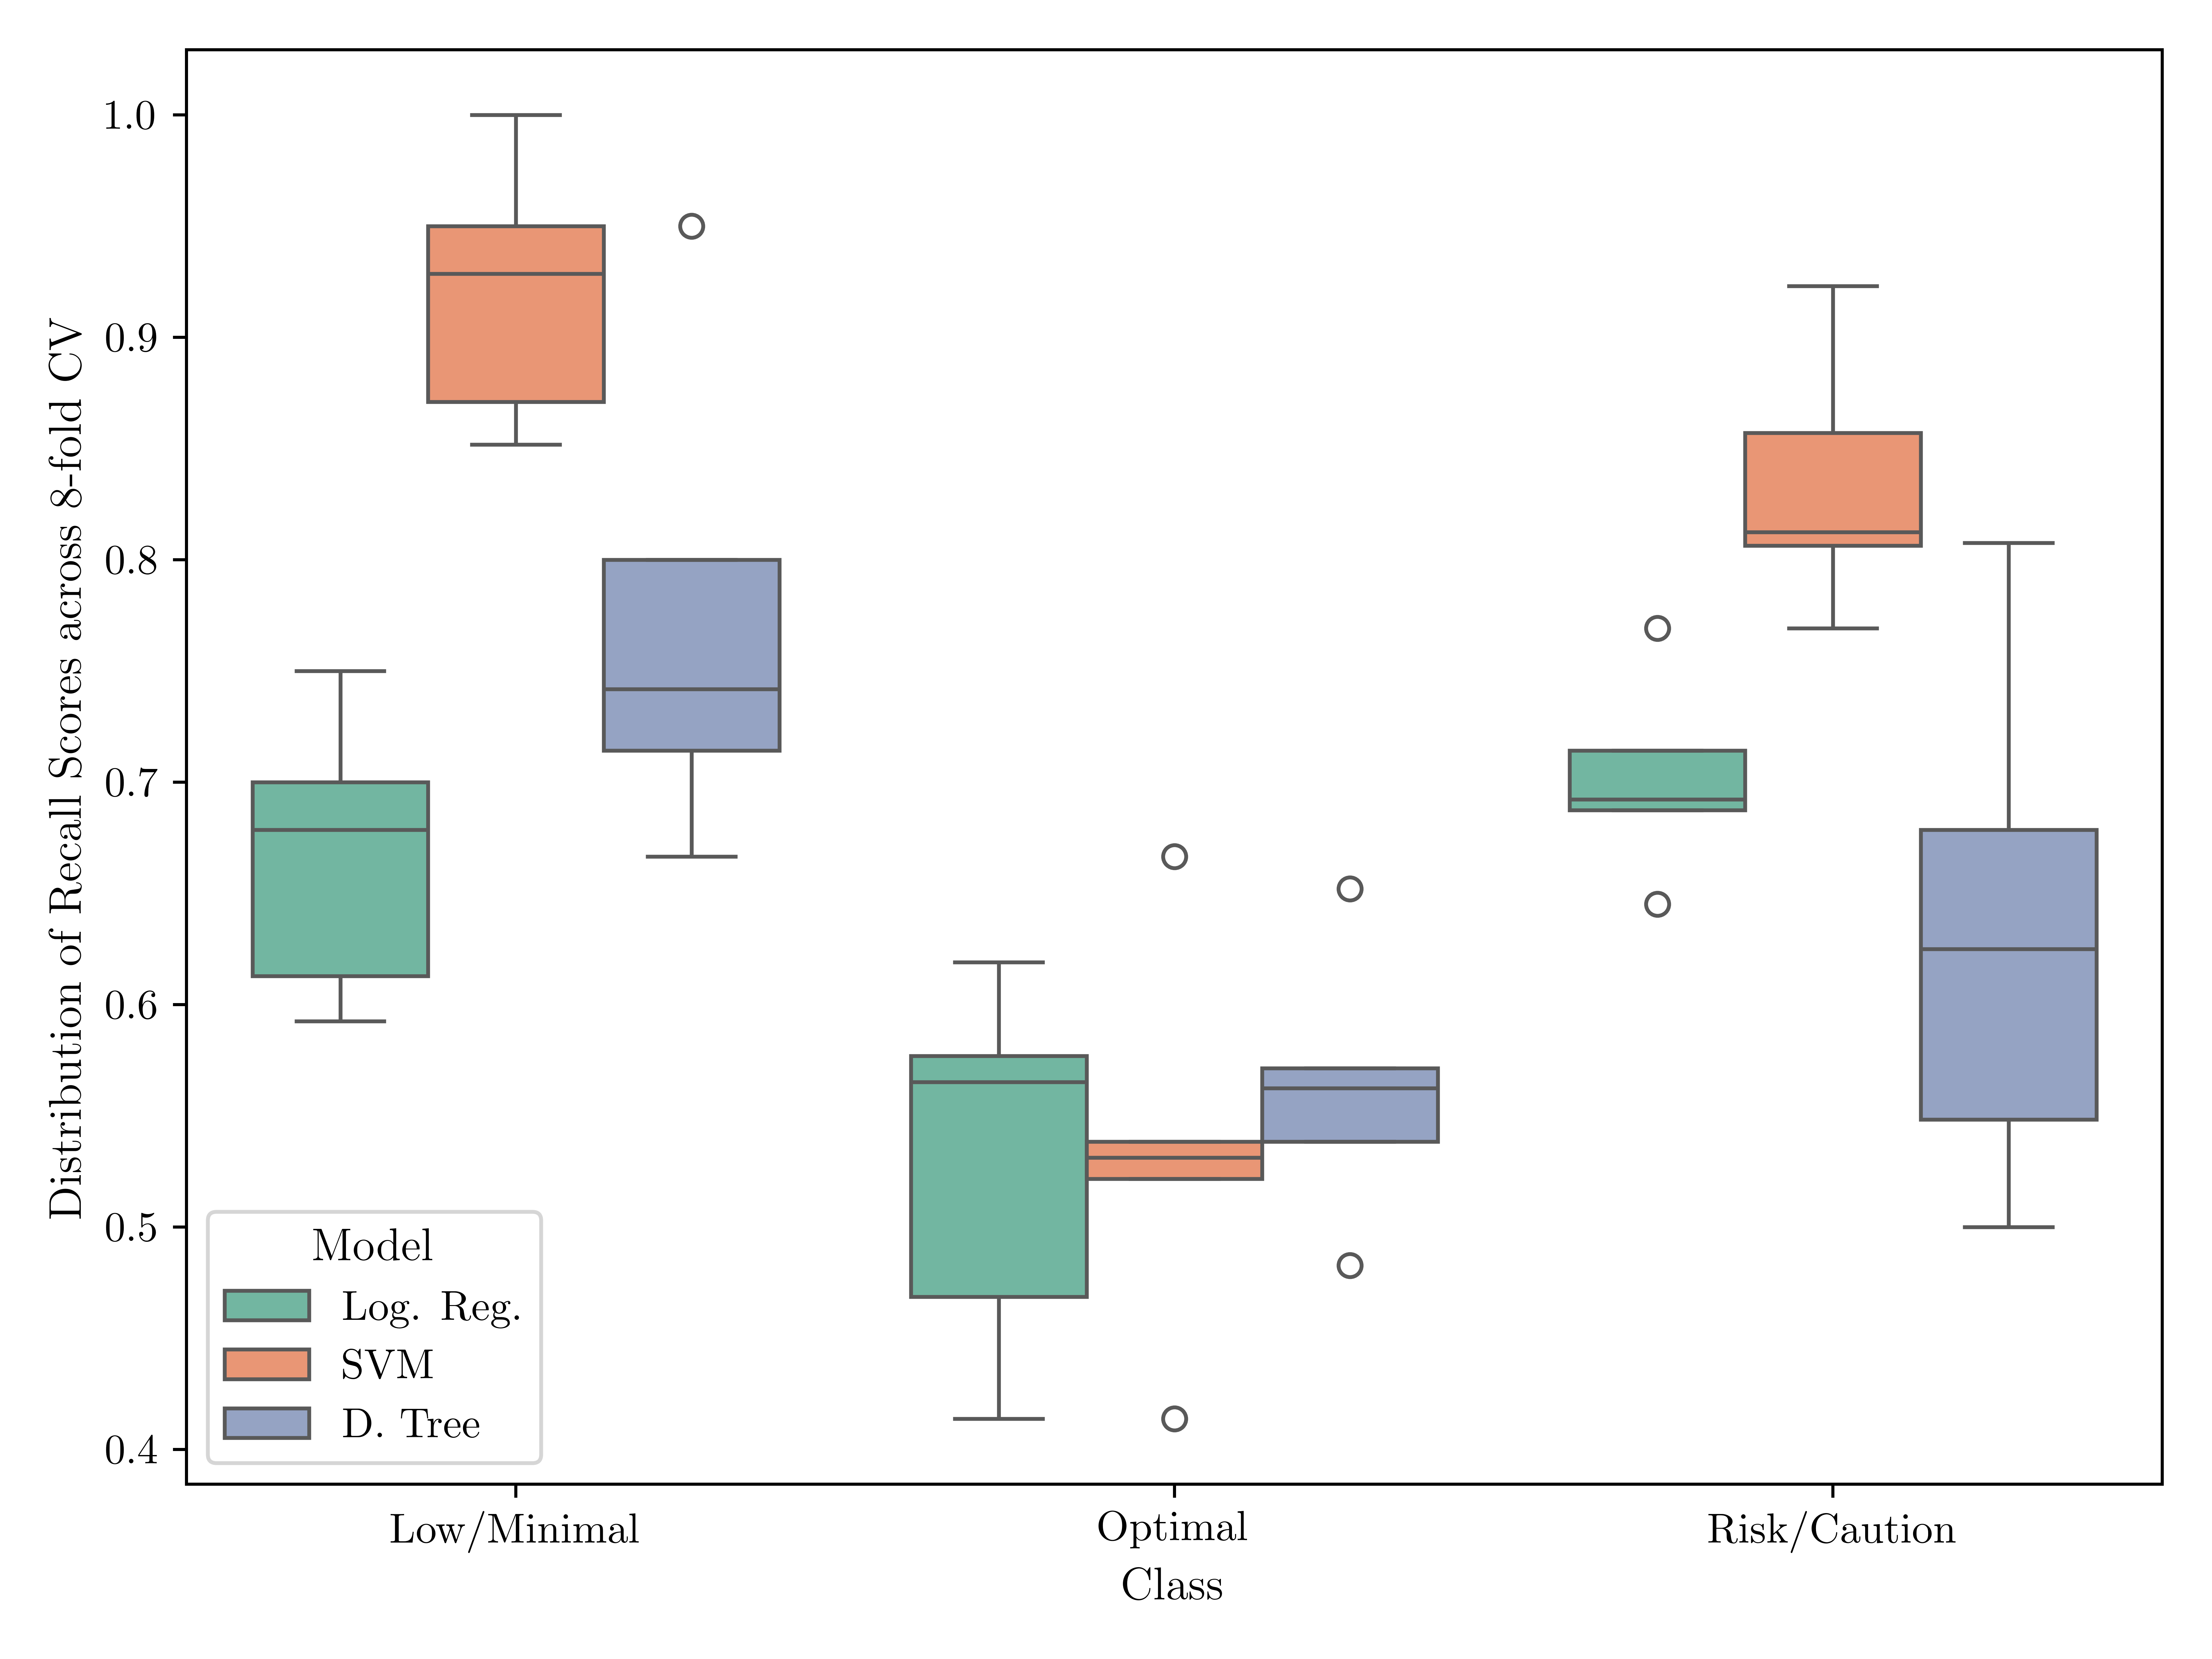
\includegraphics[width=1\linewidth]{assets/box_recall.png}
        \caption{Recall scores across 8-fold cross-validation.}
        \label{box_recall}
    \end{subfigure}

    \vspace{0.5cm}

    \begin{subfigure}[1]{\linewidth}
        \centering
        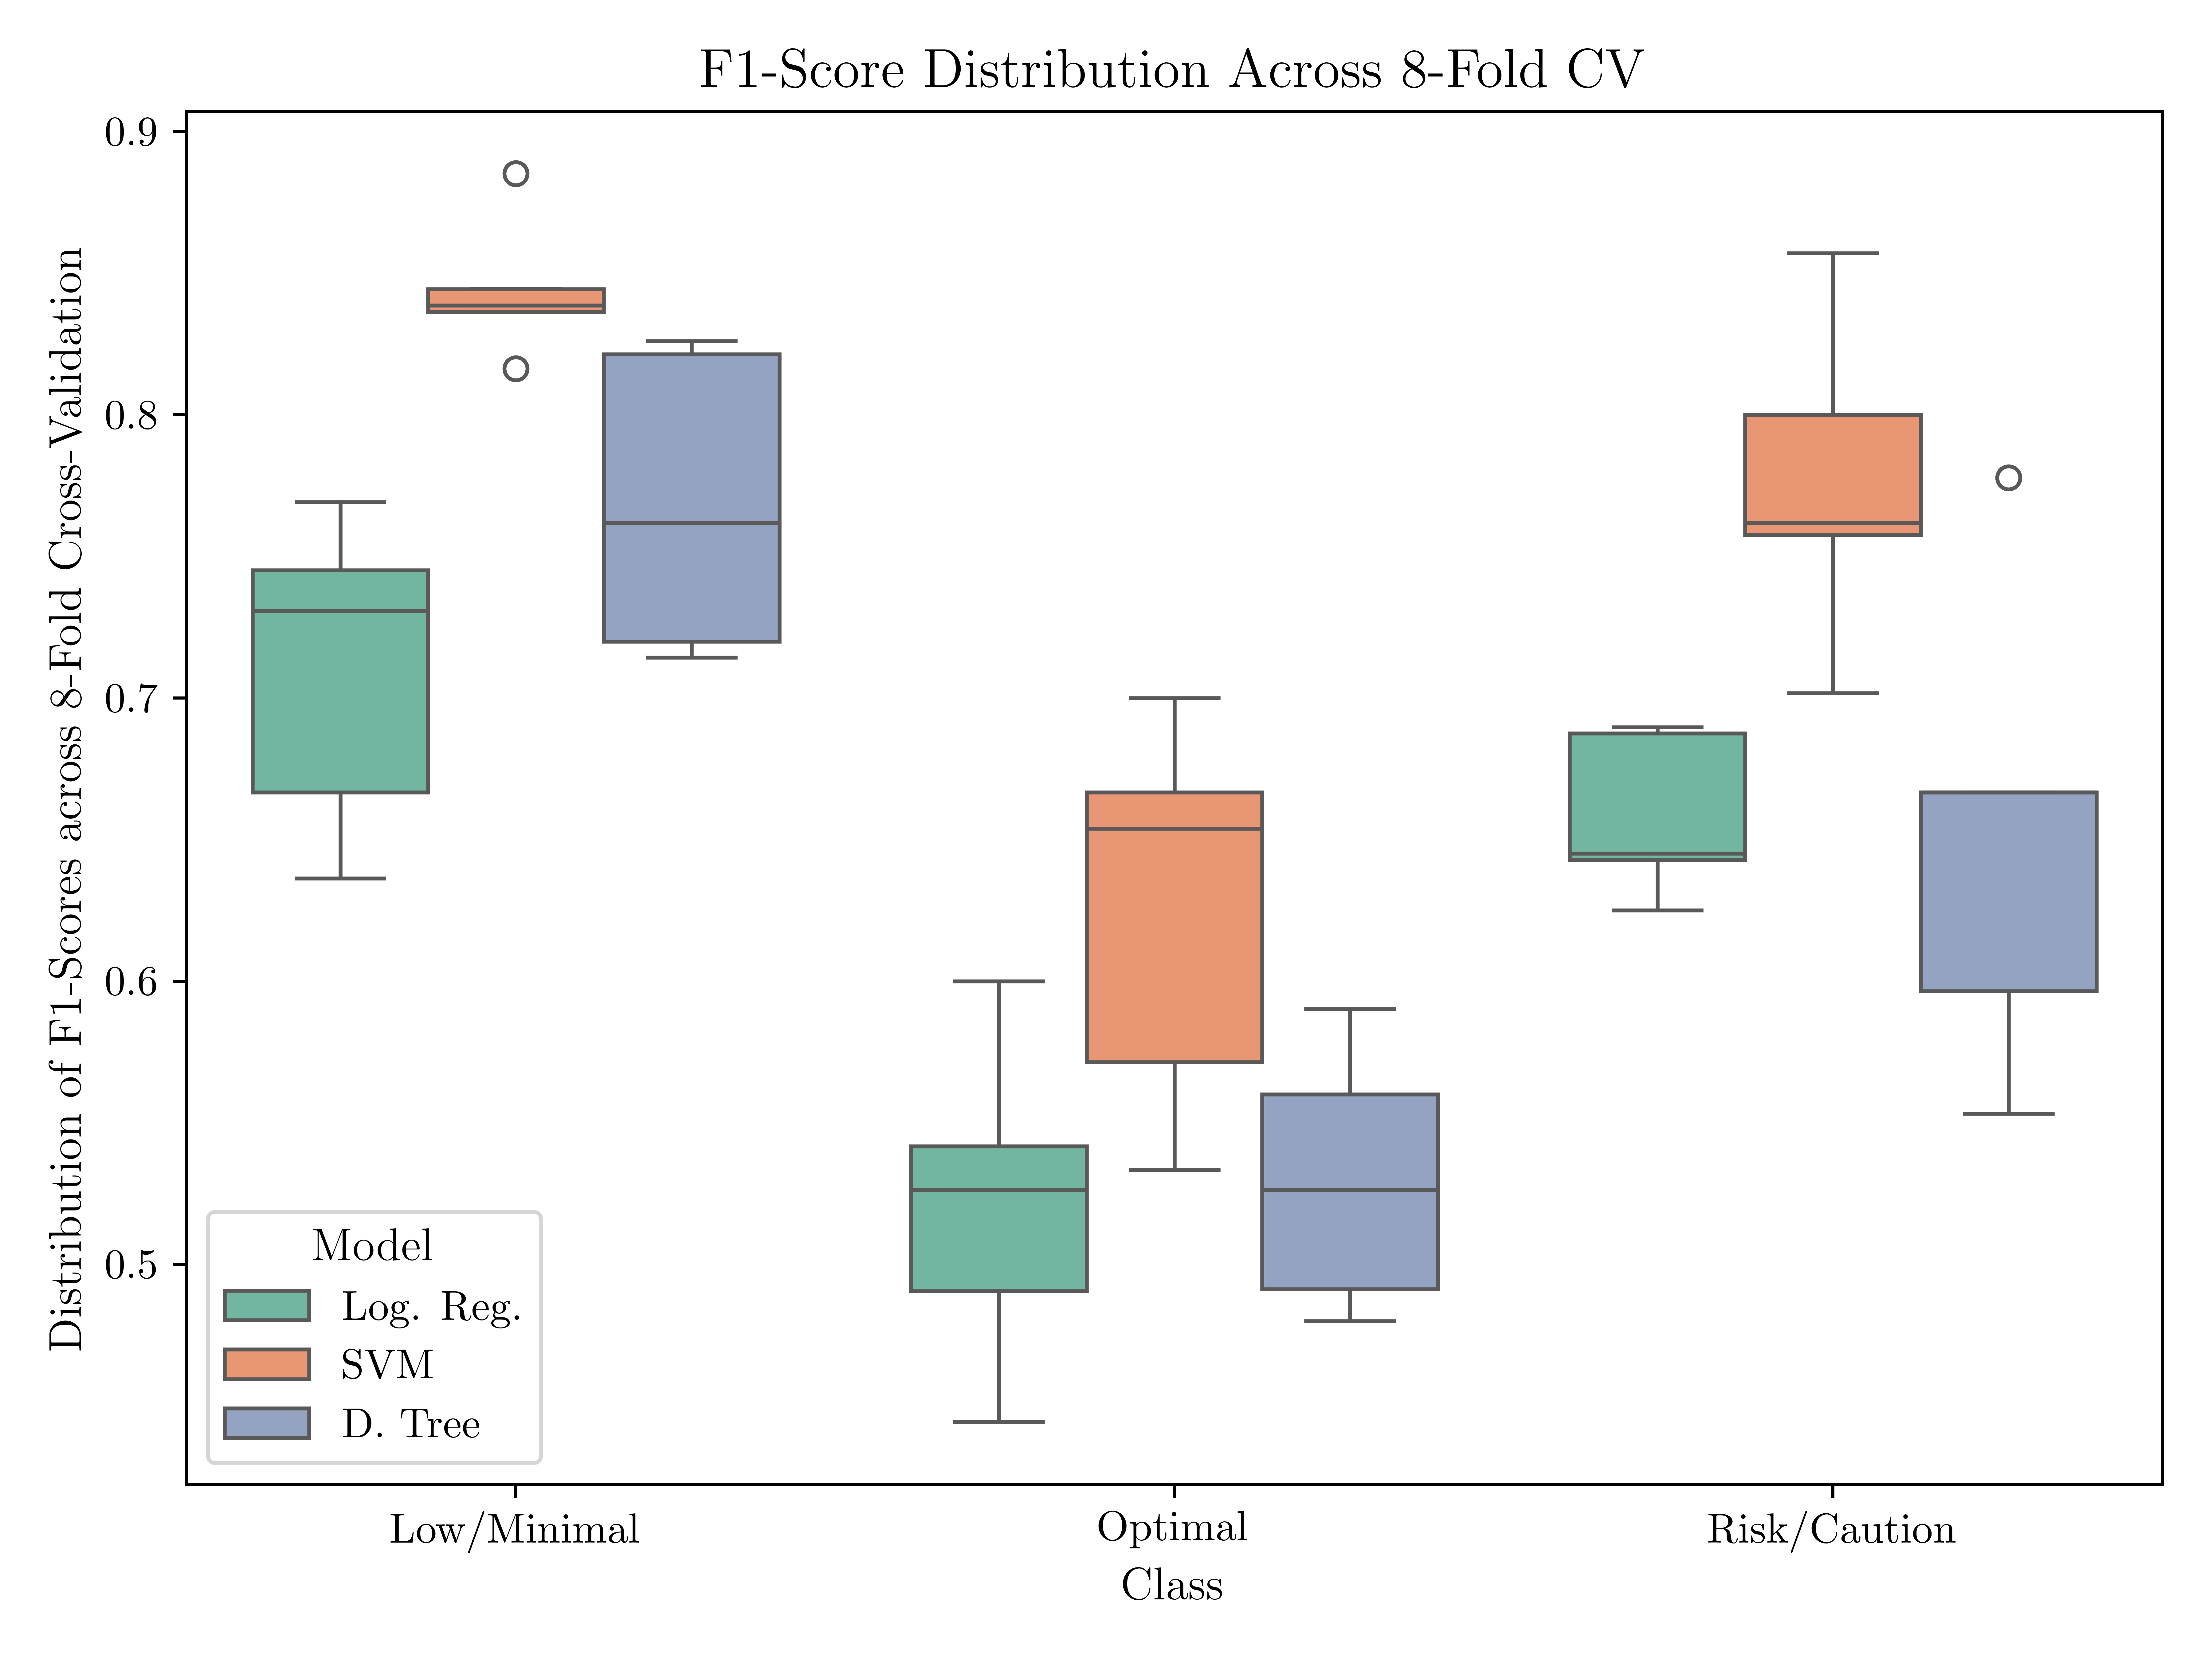
\includegraphics[width=1\linewidth]{assets/box_f1score.png}
        \caption{F1-Scores across 8-fold cross-validation.}
        \label{box_f1score}
    \end{subfigure}
    
    \caption{Boxplots showing the distribution of (a) precision, (b) recall and (c) f1-scores across 8-fold cross-validation for the different classes and models.}
    \label{box_plots1}
\end{figure}


Boxplots, comparação entre modelos tendo em vista a disparidade de performance entre classes (particularmente para LogReg e DTree)

atraves da analise dos resultados do precision, recall e f1-score, é possivel observar alguns padrões. nomeadamente:

- o modelo SVM é o que tem sempre melhores resultaods, destancando-se pela positiva em todas as métricas;

- a classe Optimal é destacada pelos seus maus resultados, revelando dificuldades na sua identificação e justificando a atribuiação dos pesos na otimizacao dos modelos.

- o modelo decision tree parece apresentar uma variância significativa nos seus resultados across all metrics, o que pode indicar que é um modelo sensível aos dados utilizados tanto no treino como no teste

é importante referir que estas variacoes na variacao se deve ao facto de fazer 8-folds, e nao termos muitos dados, acaba por haver um desvio padrao maior nos resultados, por serem menos dados a ser testados

para alem disso , Facto de o nosso dataset ter dados repetidos para a class low/minmal, apesar de uma quantidade pouco significativa ($12.5\%$), pode ocorrer ele ser treinado em dados q também irá testar, podendo haver um enviesamento positivo nas suas metricas.

\begin{figure}[H]
    \centering
    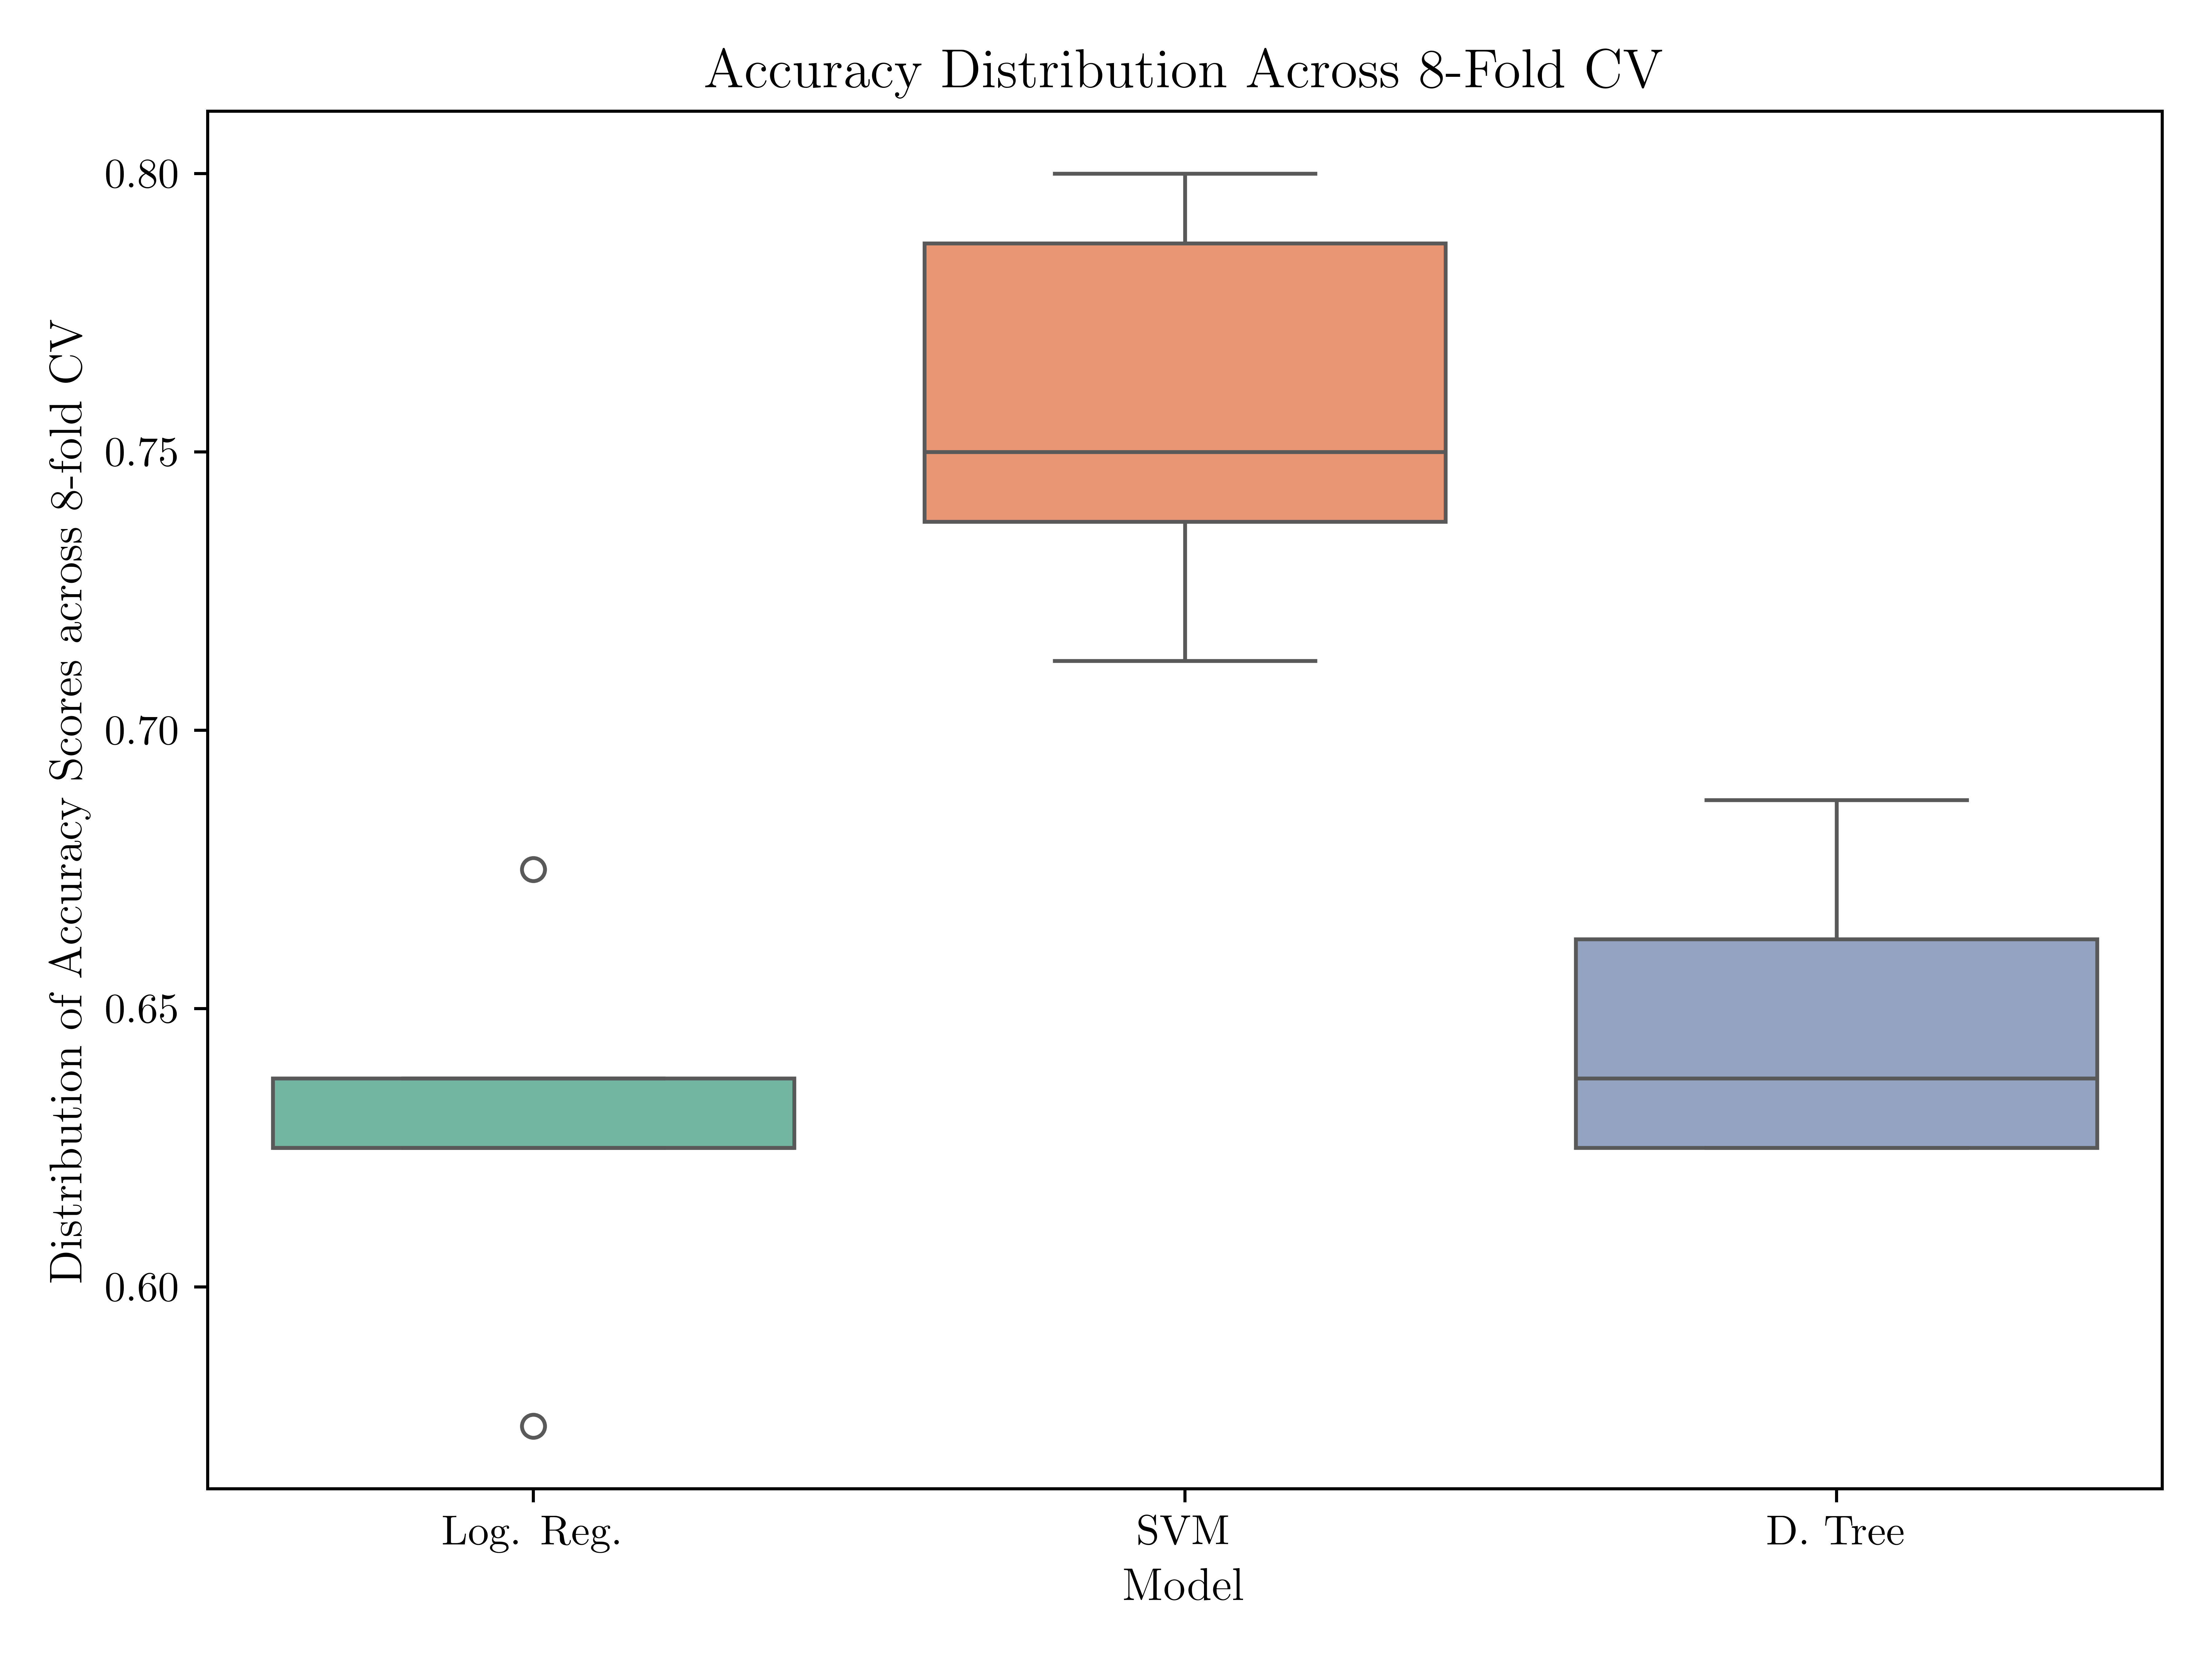
\includegraphics[width=1\linewidth]{assets/box_accuracy.png}
    \caption{Boxplots showing the distribution of accuracy scores across 8-fold cross-validation for different models.}
    \label{box_accuracy}
\end{figure}

de forma mais direta, através do accuracy, verifica-se mais uma vês o destaque do desemepnho do modelo SVM quando comparado aos restantes, pelo que será o melhor modelo obtido.

\subsection{representao no espaço?}

em vista a auferir as razoes por detras de algumas conclusoes a partir dos resultados expressos acima, decidiu-se representar the decision boundaries for each model on principal component axes, tal como os dados de teste e respetivas classificacoes reais. é importante notar que the decision boundaries são uma aproximação, uma vez que foi aplicado o PCA retendo apenas as duas primeiras direções, pelo que alguma da variação foi perdidade na criação dos decision boundaries, sendo perdido algum desempenho do modelo na visualização gráfica.

atraves da analise das seguintes figuras, pode-se verificar entao no fundo uma aproximacao do decision bondarie no espaço das componentes pricipains, revelando que categoriza as observacacoes mais a esquerda como low/minimal, as do meio como optimal, e as mais a direita como risk/caution (NS SE SE META ISSO, QUERIA FAZER UMA INTERPRETACAO MAIS GERAL DE TODOS IDK, OQ ACHAS?)

\begin{figure}[H]
    \centering
    \includegraphics[width=1\linewidth]{assets/pca_reglog.png}
    \caption{Approximation of decision boundaries for logistic regression on principal component axes, showing true and predicted classes.}
    \label{pca_reglog}
\end{figure}

No caso da análise da Regressão Logística, observa-se uma maior precisão na classificação da classe Low/Minimal, o que também é confirmado pelo boxplot correspondente, que mostra uma mediana mais alta para essa classe em comparação com as outras. Isso indica que o modelo apresenta um desempenho relativamente consistente e confiável ao classificar instâncias dessa classe. 

Quanto às restantes classes, Optimal e Risk/Caution, estas não parecem ter resultados tão precisos, não havendo uma separação mais significativa entre as classes, indicando que o modelo tem dificuldade em distinguir claramente entre essas classes, especialmente quando se observa a distribuição das previsões e as misclassifications no gráfico.


\begin{figure}[H]
    \centering
    \includegraphics[width=1\linewidth]{assets/pca_svm.png}
    \caption{Approximation of SVM decision boundaries on principal component axes, showing true and predicted classes.}
    \label{pca_svm}
\end{figure}

Através da análise da figura \ref{pca_svm}, é possível observar claramente o comportamento do kernel RBF no SVM, evidenciado pela delimitação mais precisa das fronteiras de decisão entre as classes. Esta delimitacao, e atendendo a classificacao real de cada observacao, leve a querer que haja uma melhor precisão na classificação das diferentes classes, capturando melhor as complexidades dos dados, o que também foi confimrado pelos resultados da figura \ref{box_precision}.

\begin{figure}[H]
    \centering
    \includegraphics[width=1\linewidth]{assets/pca_dtree.png}
    \caption{Approximation of decision boundaries for decision tree on principal component axes, showing true and predicted classes.}
    \label{pca_dtree}
\end{figure}

por ultimo, a decision tree apresenta decision boundaries mais complexos, o que se pode dever as suas decisões discretas, poeque ao contrário dos outros modelos, que tentam ajustar uma superfície contínua para separar as classes, o decision tree divide o espaço de características de forma hierárquica e discreta, poeque em cada nó da árvore acontece uma divisao baseadas em condições binárias

embora a dtree seja um modelo poderoso para capturar relações não-lineares, a sua representação gráfica neste contexto mostra que enfrenta dificuldades para separar claramente as observações entre as classes, com exceção da classe "Risk/Caution", que apresenta um comportamento mais favorável.

AUMENTO DIMENSIONALIDADE E OVERFITING ?

sobre todos: 

Estas análises gráficas ajudam a perceber a complexidade do problema e a dificuldade dos modelos em conseguir uma separação eficiente entre as classes. A sobreposição, especialmente da classe Optimal, destaca a necessidade de considerar ajustes nos modelos, transformações adicionais nos dados ou até modelos mais robustos que possam capturar melhor as relações subjacentes entre as classes e melhorar a precisão da classificação. (CONCLUSAO OU AQUI?)

\section{Conclusion}

SVM apresenta um desempenho superior, com maior consistência e precisão em relação às outras abordagens analisadas.

The conclusion goes here.

% use section* for acknowledgment
\section*{Acknowledgment}


The authors would like to thank... professora petia e treinador e organizacao do clue


\section{NOTAS}

Discussão dos resultados:
-\> Importante considerar os kernels selecionados, e o que isso pode representar dado o tamanho reduzido do nosso dataset

-> Há coerência entre métricas (F1-score Test vs Train está à mesma distância quase sempre)

-> Confusion matrix destaca SVM, em que apenas sofre na atribuição da classe real do 'Optimal', mas tende a pender mais na fronteira Optimal/Risk

-> Temos algumas zonas em branco ao longo do documento, temos de ver como resolver (não sei se será mais texto em alguma zona, mas gosto pouco de adicionar palha)

-> Movi o que tinhas nos modelos aqui para baixo para ver como começava a ficar distribuído

-> Novelty and contributions (3) Compare your solution with the works of other authors (published references) , try to propose a better solution, e.g. improve the performance of the ML model in solving the problem you work with.

SVM

Não introduzi os parâmetros como tabela, porque varia de modelo para modelo e achei que não fosse ficar tão bem. Queres indicar as expressões para todos os kernel ou só discutir brevemente? É que se não começamos a ter pano para mangas, particularmente só com o SAGA....

Nesta parte não introduziria mais texto, deixava de maneira mais simples e ilustrativa como no caso do LogReg


Considerar usar dataset com informação combinada de atletas para reter carácter temporal (progressão da época, aumento de cargas e combinação com features que tenham referência temporal [carga de treino do dia anterior]

Modelos sugeridos: Random Forest / SVM

temos com objetivo generalizar para que qq treinador possa ter nocao do comporamento e do estado dos seus atletas, podendo ajustar os seus treinos e cargas físicas consoante as medidas de fadigas.

para alem disso tbm se quer ver quais as metricas mais importantes relacionadas coma a fadiga

De acordo com a conversa com a professora é importante perceber como é que se deve definir a memória da nossa t-SNE, e a importância que isso tem no período da fadiga.

ns q dados fornecidos por um treinador de natacao, tivemos de organizar os dados em folhas de excel, visto estarem por linhas e com graficos e formulas de acordo com o treinador, bla bla, teve-se fazer oq? sabes melhor q eu pq foste tu q fizeste

os valores da fadiga foram convertidos para categoricos, pq e mais interessante classificar a fadiga, tendo em conta intervalos dados pelo treinador, do q numero que tornam mais dificl a interpretacao dos mesmos

de seguida agruparam-se os dados todos num novo ficheiro excel, para posterior analise atraves do python, de forma mais facilitata

tem se entao dados diarios, para X atletas, durante ns q tempo, ao longo da epoca tal, totalizando x observacoes (linhas)

para cada observacao tem se variaveis como ... bla bla e bla, contudo, nem todas serao usadas, devido a insights dados pelo treinador aka expert

as variaveis que irao ser utilizadas no estudo são tal tal, que representa tal, tal tal, ... ns q ns q mais.

\cite{Williams17} better way chronic load

\cite{Carey_2018} Predictive Modelling of Training Loads and Injury in Australian Football Carey 2018

\cite{Seow20} another review (Prediction models for musculoskeletal injuries in professional sporting activities: A systematic review)

\cite{Murray16} Murray et al. (2016



% trigger a \newpage just before the given reference
% number - used to balance the columns on the last page
% adjust value as needed - may need to be readjusted if
% the document is modified later
%\IEEEtriggeratref{8}
% The "triggered" command can be changed if desired:
%\IEEEtriggercmd{\enlargethispage{-5in}}


\bibliographystyle{IEEEtran}
\bibliography{references}

\end{document}



